\documentclass{article}
\usepackage{xcolor}
\usepackage{subfig}
\usepackage[boxed]{algorithm2e} 
\usepackage{graphicx}
\usepackage{arxiv           }
\usepackage{amsmath         } % allow align
\usepackage{amssymb         }
\usepackage[utf8]{inputenc  } % allow utf-8 input
\usepackage[T1]{fontenc     } % use 8-bit T1 fonts
\usepackage{url             } % simple URL typesetting
\usepackage{booktabs        } % professional-quality tables
\usepackage{amsfonts        } % blackboard math symbols
\usepackage{nicefrac        } % compact symbols for 1/2, etc.
\usepackage{microtype       } % microtypography
\usepackage{lipsum          }
\usepackage{hyperref}
\urlstyle{same}
\hypersetup{ 
    colorlinks=true,
    linkcolor=blue,
    filecolor=blue,      
    urlcolor=blue,
    citecolor=blue
} 
\newcommand\numberthis{\addtocounter{equation}{1}\tag{\theequation}}
\newcommand{\hess}{\text{Hessian}}
\newcommand{\diff}{\Delta}
\newcommand{\ind}{\text{Indicator}}%indicator
\newcommand{\bin}{\text{Boolean}}
\newcommand{\sat}{\text{Saturation}}
\newcommand{\win}{\text{Window}}
\newcommand{\dz}{\text{Deadzone}}
\newcommand{\hinge}{\text{Hinge}}
\newcommand{\sign}{\text{sign}}
\newcommand{\AND}{\quad\text{and}\quad}
\newcommand{\OR}{\quad\text{or}\quad}
\newcommand{\rbf}{\text{rbf}}
\newcommand{\nn}{\text{nn}}
\newcommand{\argmin}[1]{\underset{#1}{\text{argmin}}}
\newcommand{\img}{\text{img}}
\newcommand{\norm}[1]{\left\|#1\right\|}
\newcommand{\rbst}{\text{rbst}}
\newcommand{\svm}{\text{svm}}
\newcommand{\TODO}{\textbf{\textcolor{green}{TODO}}}
\newcommand{\LP}{\textbf{ LP }}
\newcommand{\QP}{\textbf{ QP }}
\newcommand{\QCQP}{\textbf{ QCQP }}
\newcommand{\QCLP}{\textbf{ QCLP }}
\newcommand{\SDP}{\textbf{ SDP }}
\newcommand{\SOCP}{\textbf{ SOCP }}
\newcommand{\GP}{\textbf{ GP }}
\newcommand{\LMI}{\textbf{ LMI }}
\newcommand{\NLP}{\textbf{ NLP }}
\newcommand{\CVXP}{\textbf{ CVXP }}
\newcommand{\note}[1]{\textbf{Note}: #1}
\newcommand{\true}{ \textbf{true} }
\newcommand{\false}{\ textbf{false} }
\newcommand{\brake}{ \textbf{break} } 
\newcommand{\minus}{\phantom{-}}
\newcommand{\rand}[1]{\widetilde{#1}} 
\newcommand{\sys}{\text{sys}}
\newcommand{\ctp}{{\text{c}\tp}}
\newcommand{\tr}{\text{tr}}
\newcommand{\trace}[1]{\text{tr}\left(#1\right)}
\newcommand{\eig}{\text{eig}}
\newcommand{\svd}{\text{svd}}
\newcommand{\vecf}[1]{\mathrm{vec}\left(#1\right)}
\newcommand{\grad}{\nabla}
\newcommand{\pd}[2]{ \frac{\partial #1}{\partial #2} }
\newcommand{\pdLARGE}[2]{ \dfrac{\partial #1}{\partial #2} }
\newcommand{\pdd}[3]{ \frac{\partial^2 #1}{\partial #2 \partial #3} }
\newcommand{\pddLARGE}[3]{ \dfrac{\partial^2 #1}{\partial #2 \partial #3} }
\newcommand{\mat}[1]{\left[\begin{array}{lllllllllllllllllll}#1\end{array}\right]}
\newcommand{\arr}[1]{\begin{array}{lllllllllllllllllll}#1\end{array}}
\newcommand{\sig}{s}
\newcommand{\lrs}{U_+}
\newcommand{\lns}{U_0}
\newcommand{\rrs}{V_+}
\newcommand{\rns}{V_0}
\newcommand{\psv}{S_+}
\newcommand{\rank}{\text{rank}}
\newcommand{\st}{\text{s.t.}}
\newcommand{\lb}{\text{lb}}
\newcommand{\ub}{\text{ub}}
\newcommand{\eq}{\text{eq}}
\newcommand{\e}{\textbf{e}}
\newcommand{\ones}{\textbf{1}}
\newcommand{\zeros}{\textbf{0}}
\newcommand{\eye}{\emph{\textbf{I}}}
\newcommand{\tp}{\intercal}
\newcommand{\diag}{\text{diag}}
\newcommand{\col}{\text{col}}
\newcommand{\row}{\text{row}}
\newcommand{\depth}{\text{depth}}
\newcommand{\E}[1]{\langle#1\rangle}
\newcommand{\prob}{\text{Probability}}
\newcommand{\R}{\textbf{R}}
\newcommand{\Z}{\textbf{Z}}
\newcommand{\C}{\textbf{C}}
\newcommand{\poly}{\textbf{P}}
\newcommand{\dom}{\textbf{D}}
\newcommand{\cvx}{\text{cvx}}
\newcommand{\sym}{\textbf{S}}
\newcommand{\posdef}{\textbf{S}_+}
\newcommand{\nonnegdef}{\textbf{S}_{0+}}
\newcommand{\ListBullet}{
    \renewcommand{\labelitemi}{$\bullet$}
    \renewcommand{\labelitemii}{$\bullet$}
    \renewcommand{\labelitemiii}{$\bullet$}
    \renewcommand{\labelitemiv}{$\bullet$}
    }
\title{\QP}
\author {
            Dr. Luke A.~Wendt                                       \\
            Department of Electrical and Computer Engineering       \\
            University of Illinois at Urbana-Champaign              \\
            \texttt{Luke.A.Wendt@gmail.com}                         \\
            \url{Luke-A-Wendt.info}                                 \\
        }
\begin{document}
\maketitle
\begin{abstract}

    This repo explores general formulation 
    of \LP (linear programs)  and \QP (quadratic programs)
    with applications in modeling, prediction, and control.
    These formulations have well-known solution methods that scale and 
    are fully developed technologies integrated into most programming languages
    (making them readily available for embedded applications).
    State-of-the-art implamentation uses hardware accelerated 
    distributed optimization specialized for sparse representations and parallelization.

    \keywords{ linprog \and \LP \and quadprog \and \QP }

\end{abstract}
\clearpage
\tableofcontents
\clearpage
\section{Notation}

\subsection{Sets}
\begin{align*}
    \begin{array}{ll}
        \Z&:\text{integers (zahlen)}\\
        \R&:\text{reals}\\
        \\
        \textbf{R}_+&: \text{positive}\\
        \textbf{R}_{0+}&: \text{non--negative}\\
        \\
        \R^n &:\text{column vector}\\
        \R^{m\times n} &:\text{matrix}\\
        \\
        \R[a,b] &:\{x\in\R\:|\:a\leq x\leq b\}\\
        \R(a,b) &:\{x\in\R\:|\:a<x<b\}\\
        \\
        \R[a,b]^n&: \{x_i\in\R[a,b]\:|\:i\in\Z[0,n-1]\}\\
        \{a,b\}^n&: \{x_i\in\{a,b\}\:\:|\:i\in\Z[0,n-1]\}\\
        \\
        \sym^n&: \text{symmetric matrix}\\
        \posdef^n&: \text{positive definite matrix}\\
        \nonnegdef^n&: \text{non--negative definite matrix}\\
        \\
        \poly&:\text{polyhedron}\\
        \dom&:\text{domain}
    \end{array}
\end{align*}
\subsection{Matrices}
    \begin{align*}
        \begin{array}{ll}
            \ones &:\text{ones}\\
            \zeros &:\text{zeros}\\
            \eye &:\text{identity matrix}\\
            \e &:\text{element vector}\\
            \\
            (\cdot)^\tp&:\text{transpose}\\
            (\cdot)^+ &:\text{pseudo inverse}\\
            (\cdot)_\bullet &:\text{index enumeration}\\
            \\
            \diag&:\text{block diagonal}\\
            \row&:\text{row--wise concatenation}\\
            \col&:\text{column--wise concatenation}
        \end{array}
    \end{align*}
\subsection{Probability}
    \begin{align*}
        \begin{array}{ll}
            \rand{(\cdot)}&:\text{random variable}\\
            \E{\cdot}&:\text{expectation}
        \end{array}
    \end{align*}
\subsection{Optimization}
    \begin{align*}
        \begin{array}{ll}
            (\cdot)^\circ   &:\text{target solution}\\
            (\cdot)^*       &:\text{optimal solution}
        \end{array}
    \end{align*}
\subsection{Functions}
    \begin{align*}
        \bin(x\in\dom)
        &=\left\{
            \arr{
            1&\text{if $x\in\dom$} \\ 
            0&\text{else}
            }\right.
            &&\text{}
            \\\\
        \ind(x\in\dom)&=-\log(\bin(x\in\dom))\\
        &=\left\{
            \arr{
            0&\text{if $x\in\dom$} \\ 
            \infty&\text{else}
            }\right.
            &&\text{}\\\\
        (x)_+&=\left\{
            \arr{
            x&\text{if $x>0$} \\ 
            0&\text{else}
            }\right.&&\text{hinge}
        \\\\
        \dz(x,a,b)&=(x-b)_+-(-x-a)_+,\quad\text{for}\quad a<0<b
        &&\text{}
        \\\\
        \sat(x,a,b)&=
        \left\{
            \arr{
                b&\text{if $x>b$} \\ 
        a&\text{if $x<a$} \\
        x & \text{else}}\right.,\quad\text{for}\quad\:a<b
        &&\text{}
        \\\\
        \win(x,a,b)&=
        \bin(x\in\R[a,b]),
                \quad\text{for}\quad\:a<b
        &&\text{}
    \end{align*} 

    \note{For the $\dz()$, $\sat()$, and $\win()$ functions,}

    \begin{align*}
        f(x,c)&=f(x,-c,c),\\
        f(x)&=f(x,1).
    \end{align*}   

    \begin{figure}[b!]
        \centering
        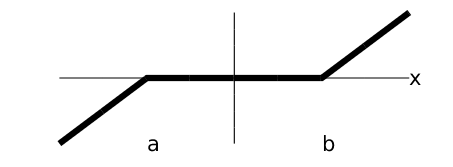
\includegraphics[width=0.3\textwidth]{./figs/deadzone_linear.png}
        \caption{$\dz$}
        \label{fig:deadzone_linear}
    \end{figure}
    \begin{figure}[b!]
        \centering
        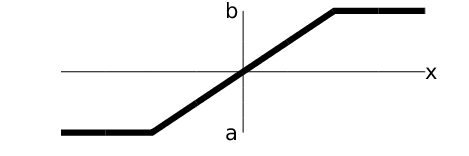
\includegraphics[width=0.3\textwidth]{./figs/sat.png}
        \caption{$\sat$}
        \label{fig:sat}
    \end{figure}
    \begin{figure}[b!]
        \centering
        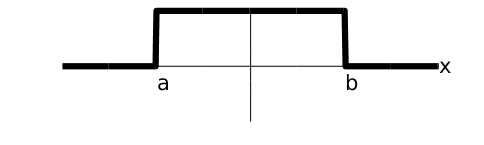
\includegraphics[width=0.3\textwidth]{./figs/win.png}
        \caption{$\win$}
        \label{fig:deadzone_linear}
    \end{figure}

    \clearpage

\section{Introduction}

\subsection{Polyherons}
Polyheron sets are defined by
\begin{align*}
    \poly := \left\{x\in\R^n \left|
            \arr{
            A_\ub x\leq b_\ub,\\
            A_\eq x = b_\eq,\\
            x_\lb \leq x \leq x_\ub
            }
    \right\}\right.. 
\end{align*}

\subsection{\LP: Linear Programming}

    Linear optimization is formulated as \cite[p.~146]{bv_cvxbook} 

    \begin{align*}
        \min_{x\in\R^n}\quad
        J
        &=
                c^\tp x
    \end{align*}
    \begin{align*}
        \st\quad x\in\poly,
    \end{align*}
    \note{For $x\in\R^n$ and $y\in\R^n$, $x\leq y$ implies element-wise inequality.}\\
    \note{$x_\lb$ and $x_\ub$ can be absorbed into $A_\ub$ and $b_\ub$.}\\
    The solver is called with
    \begin{align*}
        x^* = \LP(c,\poly).\text{solve()}.
    \end{align*}

\subsection{\QP: Quadratic Programming}

    Quadratic optimization is formulated as \cite[p.~152]{bv_cvxbook}  
    \begin{align*}
        \min_{x\in\R^n}\quad
        J
        &=
                \frac{1}{2} x^\tp Q x
            +
                c^\tp x
    \end{align*}
    \begin{align*}
        \st\quad x\in\poly,
    \end{align*}
    The solver is called with    
    \begin{align*}
        x^* = \QP(Q,c,\poly).\text{solve()}.
    \end{align*}

    \note{\LP is a subproblem of \QP.}
    \begin{figure}[b]
        \centering
        \subfloat[\LP]{{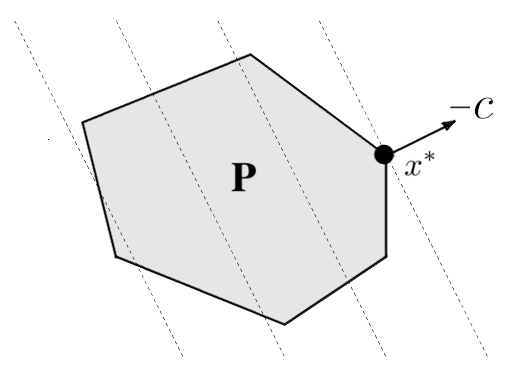
\includegraphics[width=0.42\textwidth]{./figs/LP.png} }}%
        \qquad
        \subfloat[\QP]{{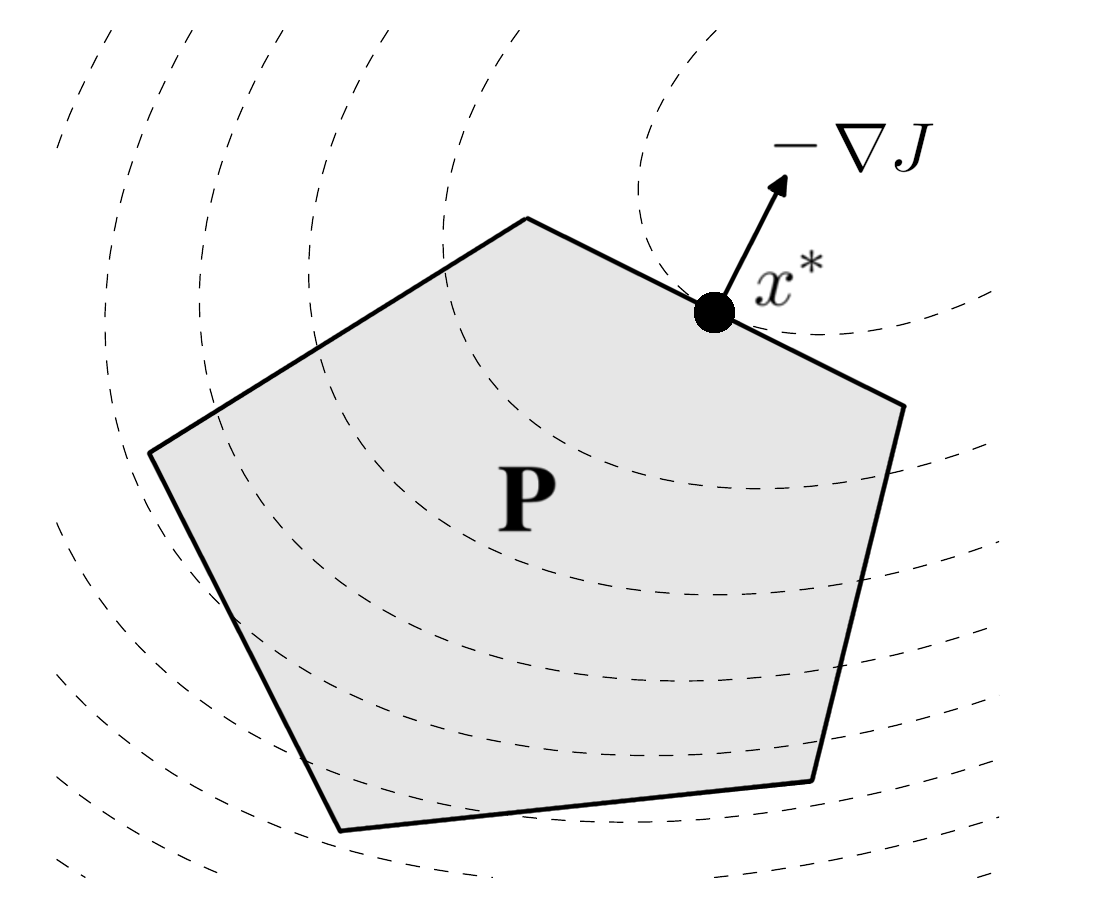
\includegraphics[width=0.4\textwidth]{./figs/QP.png} }}%
        \caption{Comparison of \LP and \QP}%
        \label{fig:LPvsQP}%
    \end{figure}

\clearpage

\section{Linear p--Norms}
    \begin{figure}[h!]
        \centering
        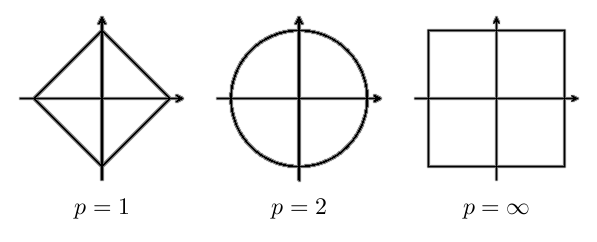
\includegraphics[width=0.5\textwidth]{./figs/norm/lp.png}
        \caption{$\|\cdot\|_p = $ constant.}
        \label{fig:lp}
    \end{figure}
    For $p\in\{1,2,\infty\}$, consider 
    \begin{align*}
            \min_{x\in\R^n}
        \quad
            J
        &=
            \|A x - b \|_p,
    \end{align*}
    \begin{align*}
        \st\quad&x\in\poly.
    \end{align*}

    The $\ell_p$ contours are depicted in Figure \ref{fig:lp}.
    The weighted linear p--norm is given by

    \begin{align*}
        \|Ax-b\|_{p,W}=\|W(Ax-b)\|_p.
    \end{align*}

    For $w_i>0$, a typical choice of weighting is
    \begin{align*}
        W=\diag\{w_i\}_{i=0}^{m-1}.
    \end{align*}

\subsection{Linear 2--Norm}

    For $x\in\R^n$, 
    \begin{align*}
            \left\| x \right\|_2^2 
        :=
            \sum_{i=0}^{n-1} x_i^2.
    \end{align*} 
    For $A\in\R^{m\times n}$,
    \begin{align*}
            \min_{x\in\R^n}
        \quad 
            J 
        &=  
            \|Ax-b\|_2^2
    \end{align*}
    \begin{align*}
        \st\quad &x\in\poly,
    \end{align*}
    is the \QP
    \begin{align*}
        \min_{x\in\R^n}\quad J 
    &=
        (Ax-b)^\tp (Ax-b)              
    \\
    &=
            x^\tp A^\tp A x 
        -   2b^\tp Ax 
        +   b^\tp b\\
    &=\frac{1}{2}x^\tp Q x +c^\tp x + r
    \end{align*}
    \begin{align*} 
        \st\quad &x\in\poly,
    \end{align*}
    where
    \begin{align*}
    Q &= \minus 2A^\tp A,\\
    c &= -2A^\tp b,\\
    r &= \minus b^\tp b. 
    \end{align*}

    \subsubsection{Weight}
    For non--negative definite $M=W^\tp W$, 

    \begin{align*}
        \|Ax-b\|_{2,W}^2 
        &=\|W(Ax-b)\|_2^2\\
        &=(Ax-b)^\tp W^\tp W (Ax-b)\\
        &= (Ax-b)^\tp M (Ax-b)\\
        &= x^\tp A^\tp M A x - 2 b^\tp M A x + b^\tp M b,
    \end{align*}
    which gives
    \begin{align*}
        Q&=\minus 2 A^\tp M A,\\
        c&=-2A^\tp M b.
    \end{align*}

    \subsubsection{Expectation}

    Consider the addition of random variables.
    The expected linear 2--norm is given by

    \begin{align*}
        \min_{x\in\R^n}\quad J&=\E{\|(A+\rand{A})(x+\rand{x})-(b+\rand{b})\|_{2,W}^2}
    \end{align*}
    \begin{align*}
        \st\quad x\in\poly,
    \end{align*}

    which, for non--negative definite $M=W^\tp W$, can be solved as the \QP

    \begin{align*}
        \min_{x\in\R^n}\quad J&=x^\tp\E{(A+\rand{A})^\tp M (A+\rand{A})}x\\
        &\quad+
        2\E{(A+\rand{A})^\tp M ((A+\rand{A})\rand{x}-(b+\rand{b}))}^\tp x\\
        &\quad+
        \E{((A+\rand{A})\rand{x}
        -(b+\rand{b}))^\tp M ((A+\rand{A})\rand{x}
        -(b+\rand{b}))}\\\\
        &=\frac{1}{2}x^\tp Q x + c^\tp x + r
    \end{align*}  
    \begin{align*}
        \st\quad x\in\poly,
    \end{align*}  
    where    
    \begin{align*}
        Q   &=2A^\tp M A + 2A^\tp M \E{\rand{A}} + 2\E{\rand{A}^\tp} M A + 2\E{\rand{A}^\tp M \rand{A} },\\
        \\
        c&=
        2\left(A^\tp MA\E{\rand{x}}
        +A^\tp M\E{\rand{A}\rand{x}}
        +\E{\rand{A}^\tp MA\rand{x}}
        +\E{\rand{A}^\tp M\rand{A}\rand{x}}\right)\\
        &\quad
        -2\left(A^\tp Mb
        +\E{\rand{A}^\tp} Mb
        +A^\tp M\E{\rand{b}}
        +\E{\rand{A}^\tp M\rand{b}}\right),
    \end{align*}
    and
    \begin{align*} 
    \begin{array}{ll}
            \vecf{\E{\rand{A}^\tp M \rand{A} }}^\tp
                &=\vec{M}^\tp\E{\rand{A}\otimes \rand{A}} ,\\
            \vecf{\E{\rand{A}^\tp MA\rand{x}}}^\tp
                &=\vecf{MA}^\tp\E{\rand{A}\otimes \rand{x}},\\
            \vecf{\E{\rand{A}^\tp M\rand{A}\rand{x}}}^\tp
                &=\vec{M}^\tp\E{ \rand{A} \otimes \rand{A}\rand{x} },\\
            \vecf{\E{\rand{A}^\tp M\rand{b}}}^\tp
                &=\vec{M}^\tp\E{\rand{A} \otimes \rand{b}}.
    \end{array}
    \end{align*}

    If the random variables are independent,

    \begin{align*}
        \begin{array}{ll}
            \E{\rand{A}\otimes \rand{x}}
                &=\E{\:\rand{A}\:}\otimes \E{\:\rand{x}\:},\\
            \E{ \rand{A} \otimes \rand{A}\rand{x} }
                &=\E{\rand{A}\otimes \rand{A}}\left(\:\eye_n\otimes \E{\rand{x}}\:\right),\\
            \E{\rand{A} \otimes \rand{b}}
                &=\E{\:\rand{A}\:} \otimes \E{\:\rand{b}\:}.
        \end{array}
    \end{align*}

\clearpage

\subsubsection{\QP to Linear 2-Norm}

    For the constraint $x\in\poly$, consider
    \begin{align*}
        \min_{x\in\R^n}\quad J&=\frac{1}{2} x^\tp Q x + c^\tp x\\
        &=\|Ax-b\|_2^2+r,
    \end{align*}    
    with    
    \begin{align*}
        Q&=\minus 2A^\tp A,\\
        c&=-2A^\tp b.
    \end{align*}
    If $Q\in\sym^n_+$,
    using SVD, the square root of $Q$
    and its inverse can be computed with
    \begin{align*}
        Q^{1/2\minus}&=US^{1/2\minus} U^\tp,\\
        Q^{-1/2}&=U S^{-1/2} U^\tp.
    \end{align*}    
    The linear 2-norm can be expressed as
    \begin{align*}
        A&=\minus\frac{1}{\sqrt{2}}Q^{1/2},\\
        b&= -\frac{1}{\sqrt{2}}Q^{-1/2} c.
    \end{align*}
    \note{This choice of $A$ gives $A=A^\tp$.}\\
    \note{The constant offset does not affect the solution.}

\subsection{Linear 1--Norm}

    For $x\in\R^n$,
    \begin{align*}
        \left\|x\right\|_1 := \sum_{i=0}^{n-1} |x_i|.
    \end{align*}
    For $A\in\R^{m\times n}$,
    \begin{align*}
        \min_{x\in\R^n}\quad J&= \|Ax-b\|_1
    \end{align*}
    \begin{align*}
        \st\quad&x\in\poly
    \end{align*}
    is equivalent to 
    \cite[p.~294]{bv_cvxbook}
    \begin{align*}
        \min_{\{x,y\}\in\{\R^n,\R^m\}}
        \quad J &= \ones^\tp y
    \end{align*}
    \begin{align*}
        \st\quad&x\in\poly,\\ 
        -y \leq A&x-b \leq y,
    \end{align*}
    which can be expressed as the \LP
    \begin{align*}
        \min_{\{x,y\}\in\{\R^n,\R^m\}}
        \quad J &=  \left[\begin{array}{l}
                            \zeros^{n}  \\   \ones^{m}
                        \end{array}\right]^\tp
                        \left[\begin{array}{r}
                            x\\
                            y
                        \end{array}\right]
    \end{align*}
    \begin{align*}                
        \st\quad &x\in\poly,\\
            \left[\begin{array}{rr}
                        A   &   -\eye _m    \\
                        -A  &   -\eye _m 
                    \end{array}\right]
                    &\left[\begin{array}{r}
                        x\\
                        y
                    \end{array}\right]
                \leq
                    \left[\begin{array}{r}
                        b\\
                        -b
                    \end{array}\right].
    \end{align*}
    \note{For $r_i=a_i^\tp x - b_i$,
    \begin{align*}
        \|Ax-b\|_1&=
        \textstyle\sum_{i=0}^{m-1} \sign(r_i)r_i. 
    \end{align*}
    }

\subsection{Linear Inf--Norm}

    For $x\in\R^n$,
    \begin{align*}
        \left\| x \right\|_\infty := \max_{i\in\Z[0,n-1]} |x_i|.
    \end{align*}
    For $A\in\R^{m\times n}$
        \begin{align*}
            \min_{x\in\R^n}\quad J &= \|A x-b\|_\infty
        \end{align*}
        \begin{align*}
            \st\quad &x\in\poly
        \end{align*}
    is equivalent to 
    \cite[p.~294]{bv_cvxbook}
    \begin{align*}
        \min_{\{x,y\}\in\{\R^n,\R\}}\quad J&= y
    \end{align*}
    \begin{align*}
        \st\quad &x\in\poly,
        \\
        -y \ones\leq A &x-b \leq y \ones,
    \end{align*}
    which can be expressed as the \LP
    \begin{align*}
        \min_{\{x,y\}\in\{\R^n,\R\}}
        \quad J&=   \left[\begin{array}{l}
                            \zeros^{n}  \\   1
                        \end{array}\right]^\tp
                        \left[\begin{array}{r}
                            x   \\
                            y
                        \end{array}\right]
    \end{align*}
    \begin{align*}
        \st\quad &x\in\poly\\
            \left[\begin{array}{rr}
                        -A  &   -\ones^{m}   \\
                        A   &   -\ones^{m} 
                    \end{array}\right]&
                    \left[\begin{array}{r}
                    x\\
                    y
                    \end{array}\right]
                \leq
                    \left[\begin{array}{r}
                        -b  \\
                        b
                    \end{array}\right].
    \end{align*}

\subsection{Combined Linear p--Norms}

    Combinations of $p\in\{1,2,\infty\}$ result in \LP or \QP.

\subsubsection{Linear 1--1--Norm}

    For $A\in\R^{m\times n}$ and $C\in\R^{r\times n}$,
    \begin{align*}
        \min_{x\in\R^n}\quad J & = \|A x-b\|_1 + \|C x - d\|_1
    \end{align*}
    \begin{align*}
        \st\quad x\in\poly
    \end{align*}
    is equivalent to
    \begin{align*}
    \min_{\{x,y,z\}\in\{\R^n,\R^m,\R^r\}}
    \quad J & = \ones^\tp y + \ones^\tp z
    \end{align*}
    \begin{align*}
        \st\quad &x\in\poly,
        \\
        -y \leq A &x - b \leq y,\\
        -z \leq C &x - d \leq z,
    \end{align*}
    which can be expressed as the \LP
    \begin{align*}
        \min_{\{x,y,z\}\in\{\R^n,\R^m,\R^r\}} \quad 
        J & = 
        \left[\begin{array}{l}
            \zeros^n
            \\
            \ones^m
            \\
            \ones^r
        \end{array}\right]^\tp
        \left[\begin{array}{c}
            x   \\
            y \\
            z
        \end{array}\right]
    \end{align*}
    \begin{align*}
        \st\quad &x\in\poly,
        \\
        \left[\begin{array}{lll}
                -A
            &
                -\eye_m
            &
            \minus\zeros^{m\times r}
            \\
                \minus A
            &
                -\eye_m
            &
            \minus\zeros^{m\times r}
            \\
            -C
            &
            \minus\zeros^{r\times m}
            &
            -\eye_r
            \\
                \minus C
            &
            \minus\zeros^{r\times m}
            &
                -\eye_r                
        \end{array}\right]
        &
        \left[\begin{array}{c}
            x   \\
            y \\
            z
        \end{array}\right]
        \leq
        \left[\begin{array}{l}
            -b                \\
            \minus b \\
            -d \\
            \minus d
        \end{array}\right].
    \end{align*}

\subsubsection{Linear 2--2--Norm}
For $A\in\R^{m\times n}$ and $C\in\R^{r\times n}$,
\begin{align*}
    \min_{x\in\R^n}\quad J & = \|A x-b\|_2^2 + \|C x - d\|_2^2
\end{align*}
\begin{align*}
    \st\quad x\in\poly
\end{align*}
is equivalent to
\begin{align*}
\min_{x\in\R^n}
\quad J & = x^\tp (A^\tp A + C^\tp C) x - 2(b^\tp A + d^\tp C)x + b^\tp b+d^\tp d
\end{align*}
\begin{align*}
    \st\quad &x\in\poly,
\end{align*}
which is a \QP with 
\begin{align*}
    Q&=\minus 2(A^\tp A + C^\tp C),\\
    c&=- 2( A^\tp b + C^\tp d).
\end{align*}

\subsubsection{Linear inf--inf--Norm}

    For $A\in\R^{m\times n}$ and $C\in\R^{r\times n}$,
    \begin{align*}
        \min_{x\in\R^n}\quad J & = \|A x-b\|_\infty + \|C x - d\|_\infty
    \end{align*}
    \begin{align*}
        \st\quad x\in\poly
    \end{align*}
    is equivalent to
    \begin{align*}
    \min_{\{x,y,z\}\in\{\R^n,\R,\R\}}
    \quad J & = y + z
    \end{align*}
    \begin{align*}
        \st\quad &x\in\poly,
        \\
        -y\ones^m \leq A &x - b \leq y\ones^m,\\
        -z\ones^r \leq C &x - d \leq z\ones^r,
    \end{align*}
    which can be expressed as the \LP
    \begin{align*}
        \min_{\{x,y,z\}\in\{\R^n,\R,\R\}} \quad 
        J & = 
        \left[\begin{array}{l}
            \zeros^n
            \\
            1
            \\
            1
        \end{array}\right]^\tp
        \left[\begin{array}{c}
            x   \\
            y \\
            z
        \end{array}\right]
    \end{align*}
    \begin{align*}
        \st\quad &x\in\poly,
        \\
        \left[\begin{array}{lll}
                -A
            &
                -\ones^m
            &
            \minus\zeros^{m}
            \\
                \minus A
            &
                -\ones^m
            &
            \minus\zeros^{m}
            \\
            -C
            &
            \minus\zeros^{r}
            &
            -\ones^r
            \\
                \minus C
            &
            \minus\zeros^{r}
            &
                -\ones^r                
        \end{array}\right]
        &
        \left[\begin{array}{c}
            x   \\
            y \\
            z
        \end{array}\right]
        \leq
        \left[\begin{array}{l}
            -b                \\
            \minus b \\
            -d \\
            \minus d
        \end{array}\right].
    \end{align*}

\subsubsection{Linear 1--2--Norm}

    For $C\in\R^{m\times n}$,
    \begin{align*}
        \min_{x\in\R^n}\quad J & =     \|A x-b\|_2^2
                        +   \|C x - d\|_1
    \end{align*}
    \begin{align*}
        \st\quad x\in\poly
    \end{align*}
    is equivalent to
    \begin{align*}
    \min_{\{x,y\}\in\{\R^n,\R^m\}}
    \quad J & =     x^\tp A^\tp A x 
                    -   b^\tp A x
                    +   b^\tp b
                    +   \ones^\tp y
    \end{align*}
    \begin{align*}
        \st\quad &x\in\poly,
        \\
        -y \leq C &x - d \leq y,
    \end{align*}
    which can be expressed as the \QP
    \begin{align*}
        \min_{\{x,y\}\in\{\R^n,\R^m\}} \quad 
        J & = \frac{1}{2}
        \left[\begin{array}{c}
            x   \\
            y
        \end{array}\right]^\tp
        \left[\begin{array}{ll}
            2A^\tp A
        &
            \zeros^{n\times m}
        \\ 
            \zeros^{m\times n}
        &
            \zeros^{m\times m}
        \end{array}\right]
        \left[\begin{array}{c}
            x   \\
            y
        \end{array}\right]
        +
        \left[\begin{array}{l}
            -2 A^\tp b
            \\
            \minus \ones^{m}
        \end{array}\right]^\tp
        \left[\begin{array}{c}
            x   \\
            y
        \end{array}\right]
        +
        b^\tp b
    \end{align*}
    \begin{align*}
        \st\quad &x\in\poly,
        \\
        \left[\begin{array}{lll}
                -C
            &
                -\eye_m
            \\
                \minus C
            &
                -\eye_m
        \end{array}\right]
        &
        \left[\begin{array}{c}
            x   \\
            y
        \end{array}\right]
        \leq
        \left[\begin{array}{l}
            -d                \\
            \minus d
        \end{array}\right].
    \end{align*}

\subsubsection{Linear 1--Inf--Norm}

    For $A\in\R^{m\times n}$ and $C\in\R^{r\times n}$,
    \begin{align*}
        \min_{x\in\R^n}\quad J & = 
                        \|A x - b\|_1
                        +   \|C x - d \|_\infty
    \end{align*}
    \begin{align*}
        \st\quad x\in\poly
    \end{align*}
    is equivalent to
    \begin{align*}
    \min_{\{x,y,z\}\in\{\R^n,\R^m,\R\}}
    \quad J & =  \ones^\tp y +z
    \end{align*}
    \begin{align*}
        \st\quad &x\in\poly,
        \\
            -y \leq A & x - b \leq y,
            \\
        -z\ones \leq C & x - d \leq z\ones,
    \end{align*}
    which can be expressed as the \LP
    \begin{align*}
        \min_{\{x,y,z\}\in\{\R^n,\R^m,\R\}} \quad 
        J & = 
        \left[\begin{array}{l}
            \zeros^{n}
            \\
            \ones^{m}
            \\
            1
        \end{array}\right]^\tp
        \left[\begin{array}{c}
            x   \\
            y   \\
            z
        \end{array}\right]
    \end{align*}
    \begin{align*}
        \st\quad &x\in\poly,
        \\
        \left[\begin{array}{lll}
                -A
            &
                -\eye_m
            &
                \minus \zeros^{m}
            \\
                \minus A
            &
                -\eye_m
            &
                \minus \zeros^{m}
            \\
                -C
            &
                \minus \zeros^{r\times m}
            &
                -\ones^{r}
            \\
                \minus C 
            & 
                \minus \zeros^{r\times m}
            &
                -\ones^{r}
        \end{array}\right]
        &
        \left[\begin{array}{c}
            x   \\
            y   \\
            z
        \end{array}\right]
        \leq
        \left[\begin{array}{l}
            -b                \\
            \minus b      \\
            -d           \\
            \minus d
        \end{array}\right].
    \end{align*}

\subsubsection{Linear 2--Inf--Norm}

    For $C\in\R^{m\times n}$,
    \begin{align*}
        \min_{x\in\R^n}\quad J & =     \|A x-b\|_2^2
                        +   \|C x - d \|_\infty
    \end{align*}

    \begin{align*}
        \st\quad x\in\poly
    \end{align*}
    is equivalent to
    \begin{align*}
    \min_{\{x,y\}\in\{\R^n,\R\}}
    \quad J & =     x^\tp A^\tp A x 
                    -   b^\tp A x
                    +   b^\tp b
                    + y
    \end{align*}

    \begin{align*}
        \st\quad &x\in\poly,\\
            -y\ones \leq    C &x - d \leq  y\ones,
    \end{align*}
    which can be expressed as the \QP
    \begin{align*}
        \min_{\{x,y\}\in\{\R^n,\R\}} \quad 
        J & = \frac{1}{2}
        \left[\begin{array}{c}
            x   \\
            y
        \end{array}\right]^\tp
        \left[\begin{array}{lll}
            2A^\tp A
        &
            \zeros^{n}
        \\ 
            \zeros^{1\times n}
        &
            0
        \end{array}\right]
        \left[\begin{array}{c}
            x   \\
            y
        \end{array}\right]
        +
        \left[\begin{array}{l}
            -2 A^\tp b
            \\
            \minus 1
        \end{array}\right]^\tp
        \left[\begin{array}{c}
            x   \\
            y
        \end{array}\right]
        +
        b^\tp b
    \end{align*}

    \begin{align*}
        \st\quad &x\in\poly,
        \\
        \left[\begin{array}{lll}
                -C
            &
                -\ones^{m}
            \\
                \minus C 
            &
                -\ones^{m}
        \end{array}\right]
        &\left[\begin{array}{c}
            x   \\
            y
        \end{array}\right]
        \leq
        \left[\begin{array}{l}
            -d           \\
            \minus d
        \end{array}\right].
    \end{align*}

\subsubsection{Linear 1--2--Inf--Norm}

    For $B\in\R^{m\times n}$ and $D\in\R^{r\times n}$,
    \begin{align*}
        \min_{x\in\R^n}\quad J & =     \|A x-b\|_2^2
                        +   \|B x - c\|_1
                        +   \|D x - e \|_\infty
    \end{align*}

    \begin{align*}
        \st\quad x\in\poly
    \end{align*}
    is equivalent to
    \begin{align*}
    \min_{\{x,y,z\}\in\{\R^n,\R^m,\R\}}
    \quad J & =     x^\tp A^\tp A x 
                    -   b^\tp A x
                    +   b^\tp b
                    +   \ones^\tp y +z
    \end{align*}

    \begin{align*}
        \st\quad &x\in\poly,
        \\
            -y \leq B &x - c \leq y,
            \\
            -z\ones \leq D &x - e \leq z\ones,
    \end{align*}
    which can be expressed as the \QP
    \begin{align*}
        \min_{\{x,y,z\}\in\{\R^n,\R^m,\R\}} \quad 
        J & = \frac{1}{2}
        \left[\begin{array}{c}
            x   \\
            y   \\
            z
        \end{array}\right]^\tp
        \left[\begin{array}{lll}
            2A^\tp A
        &
            \zeros^{n\times m}
        &
            \zeros^{n}
        \\ 
            \zeros^{m\times n}
        &
            \zeros^{m\times m}
        &
            \zeros^{m}
        \\ 
            \zeros^{1\times n}
        &
            \zeros^{1\times m}
        &
            0
        \end{array}\right]
        \left[\begin{array}{c}
            x   \\
            y   \\
            z
        \end{array}\right]
        +
        \left[\begin{array}{l}
            -2 A^\tp b
            \\
            \minus \ones^{m}
            \\
            \minus 1
        \end{array}\right]^\tp
        \left[\begin{array}{c}
            x   \\
            y   \\
            z
        \end{array}\right]
        +
        b^\tp b
    \end{align*}

    \begin{align*}
        \st\quad &x\in\poly,\\
        \left[\begin{array}{lll}
                -B
            &
                -\eye_m
            &
                \minus \zeros^{m}
            \\
                \minus B
            &
                -\eye_m
            &
                \minus \zeros^{m}
            \\
                -D
            &
                \minus \zeros^{r\times m}
            &
                -\ones^{r}
            \\
                \minus D 
            & 
                \minus \zeros^{r\times m}
            &
                -\ones^{r}
        \end{array}\right]
        &
        \left[\begin{array}{c}
            x   \\
            y   \\
            z
        \end{array}\right]
        \leq
        \left[\begin{array}{l}
            -c                \\
            \minus c      \\
            -e           \\
            \minus e
        \end{array}\right].
    \end{align*}

\subsection{Linear p--Norm Constraint} \label{sec:lin_p_norm}


    For $A_i\in\R^{m_i\times n}$ and $t_i>0$, consider the problem

    \begin{align*}
        \min_{x\in\R^n} \quad J = f(x)
    \end{align*}
    \begin{align}
        \st\quad x&\in\poly,\nonumber\\
        \|A_i&x-b_i\|_p\leq t_i.\label{eqn:p_norm_constraint}
    \end{align}

    \begin{figure}[h!]
        \centering
        \subfloat[1--norm]{{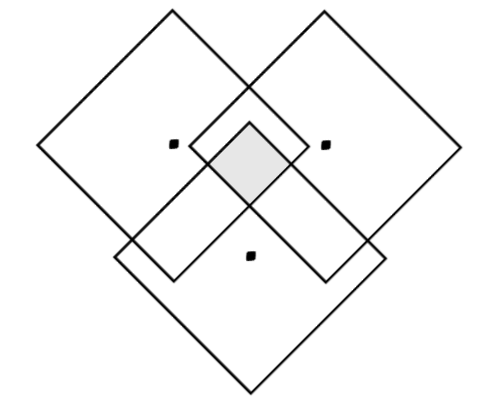
\includegraphics[width=0.25\textwidth]{./figs/norm/1_norm_constraint.png}}\label{fig:1_norm_constraint}}%
        \qquad
        \subfloat[2--norm]{{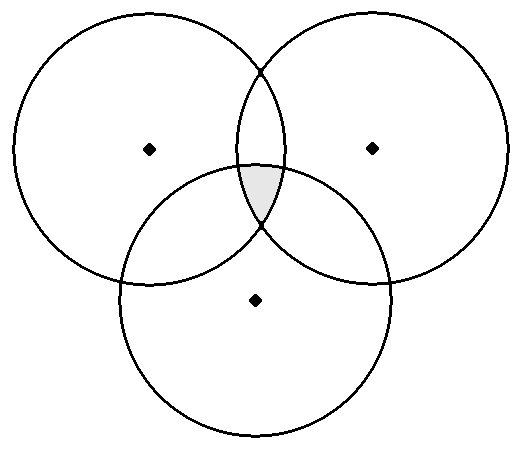
\includegraphics[width=0.25\textwidth]{./figs/norm/2_norm_constraint.png}}\label{fig:2_norm_constraint}}%
        \qquad
        \subfloat[inf--norm]{{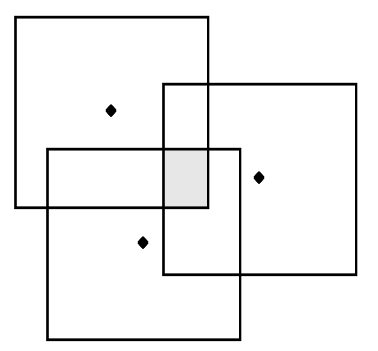
\includegraphics[width=0.2\textwidth]{./figs/norm/inf_norm_constraint.png}}\label{fig:inf_norm_constraint}}%
        \caption{Comparison of p--norm inequality constraints}%
        \label{fig:LPvsQP}%
    \end{figure}

\subsubsection{Linear 1--Norm Constraint}

    For $p=1$, Equation [\ref{eqn:p_norm_constraint}] is equivalent to

    \begin{align*}
        \min_{\{x,y_i\}\in\{\R^n,\R^{m_i}\}} \quad J =f(x)
    \end{align*}
    \begin{align*}
        \st\quad x&\in\poly,\\
        \ones^\tp y_i&\leq t_i,\\
        -y_i&\leq A_ix-b_i\leq y_i.
    \end{align*}

    Figure \ref{fig:1_norm_constraint} depicts the intersection of 1--norm inequality constraints.

    If $f(x)$ is linear, this problem is an \LP.

    If $f(x)$ is quadratic, this problem is a \QP.

\subsubsection{Linear 2--Norm Constraint}
    For $p=2$, Equation [\ref{eqn:p_norm_constraint}] can be squared to get

    \begin{align*}
        \|A_i&x-b_i\|_2^2\leq t_i^2,
    \end{align*}
    which can be expressed as
    \begin{align*}
        \frac{1}{2} x^\tp Q_i x + c_i^\tp x + r_i \leq 0,
    \end{align*}
    where
    \begin{align*}
        Q_i&=\minus 2A_i^\tp A_i,\\
        c_i&= -2A_i^\tp b_i,\\
        r_i&= \minus b_i^\tp b_i-t_i^2.
    \end{align*}

    Figure \ref{fig:2_norm_constraint} depicts the intersection of 
    2--norm inequality constraints.

    If $f(x)$ is quadratic, this problem is a \QCQP.
    
\subsubsection{Linear Inf--Norm Constraint}

    For $p=\infty$, Equation [\ref{eqn:p_norm_constraint}] is equivalent to

    \begin{align*}
        \min_{\{x,y_i\}\in\{\R^n,\R\}} \quad J =f(x)
    \end{align*}
    \begin{align*}
        \st\quad x&\in\poly,\\
        y_i&\leq t_i,\\
        -y_i\ones&\leq A_ix-b_i\leq y_i\ones.
    \end{align*}

    Figure \ref{fig:inf_norm_constraint} depicts the intersection of 
    inf--norm inequality constraints.

    If $f(x)$ linear, this problem is an \LP.

    If $f(x)$ quadratic, this problem is a \QP.

    \clearpage
    \subsection{Piecewise--Linear Minimization}
        Consider the problem
        \begin{align*}
            \min_{x\in\R^n}\quad \max_{i\in\Z[0,m-1]} \quad J_i = a_i^\tp x-b_i,
        \end{align*}
        \begin{align*}
            \st\quad x\in\poly.
        \end{align*}
        This problem is equivalent to the \LP \cite[p.~150]{bv_cvxbook}
        \begin{align*}
            \min_{\{x,y\}\in\{\R^n,\R\}} y
        \end{align*}
        \begin{align*}
            \st\quad x&\in\poly,\\
            a_i^\tp x-b_i &\leq y,
        \end{align*}
        which can be expressed as
        \begin{align*}
            \min_{\{x,y\}\in\{\R^n,\R\}} \mat{\zeros^n \\ 1}^\tp \mat{x\\y}
        \end{align*}
        \begin{align*}
            \st\quad x&\in\poly,\\
            \mat{A&-\ones^m}&\mat{x\\y}\leq b,
        \end{align*}
        where
        \begin{align*}
            A &= \row\{a_i^\tp\}_{i=0}^{m-1},\\\\
            b &= \row\{b_i\}_{i=0}^{m-1}.
        \end{align*}

\subsection{Robust p--Norm from a Finite Set}

        For $A_i\in\R^{q_i\times n}$, consider the problem
        \begin{align*}
            \min_{x\in\R^n}\quad \max_{i\in\Z[0,m-1]} \quad J_i = \|A_ix-b_i\|_p,
        \end{align*}
        \begin{align*}
            \st\quad x\in\poly.
        \end{align*}
        This problem is equivalent to \cite[p.~321]{bv_cvxbook}
        \begin{align*}
            \min_{\{x,y\}\in\{\R^n,\R\}} y
        \end{align*}
        \begin{align}
            \st\quad x&\in\poly,\nonumber\\
            \|A_ix-b_i\|_p&\leq y.\label{eqn:robust}
        \end{align}
        If $p\in\{1,\infty\}$, this is an \LP.

\subsubsection{Robust 1--Norm from a Finite Set}

        For $p=1$ and $i\in\Z[0,m-1]$, Equation [\ref{eqn:robust}] is equivalent to the \LP
        \begin{align*}
            \min_{\{x,y,z_i\}\in\{\R^n,\R,\R^{q_i}\}} \quad J =y
        \end{align*}
        \begin{align*}
            \st\quad x&\in\poly,\\
            \ones^\tp z_i&\leq y,\\
            -z_i&\leq A_ix-b_i\leq z_i.
        \end{align*}

\subsubsection{Robust Inf--Norm from a Finite Set}

        For $p=\infty$ and $i\in\Z[0,m-1]$, Equation [\ref{eqn:robust}] is equivalent to the \LP

        \begin{align*}
            \min_{\{x,y,z_i\}\in\{\R^n,\R,\R\}} \quad J =y
        \end{align*}
        \begin{align*}
            \st\quad x&\in\poly,\\
            z_i&\leq y,\\
            -z_i\ones &\leq A_ix-b_i\leq z_i\ones.
        \end{align*}


    \clearpage

\section{Penalty Functions}

    \subsection{Deadzone Penalty} 

    \begin{figure}[h!]
        \centering
        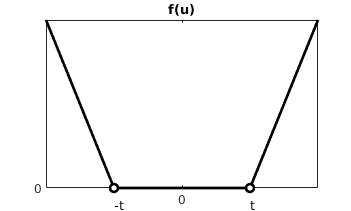
\includegraphics[width=0.5\textwidth]{./figs/norm/deadzone.png}
        \caption{Deadzone Penalty}
        \label{fig:deadzone}
    \end{figure}

    Consider the problem

    \begin{align*}
        \min_{x\in\R^n}\quad J = \sum_{i=0}^{m-1} f(a_i^\tp x - b_i)
    \end{align*}
    \begin{align*}
        \st\quad x\in\poly,
    \end{align*}

    where $f(u)$ is the deadzone

    \begin{align*}
        f(u) &= \left\{\arr{0 & \text{if $|u|\leq t$} \\ |u|-t & \text{else}}\right.\\
        &=\max(\:-u-t,\:\:0,\:u-t\:)\numberthis\label{eqn:deadzone_penalty},\\\\
        f'(u) &= \left\{\arr{0 & \text{if $|u|\leq t$} \\ \sign(u) & \text{else}}\right..
    \end{align*}
    \note{The deadzone penalty is not a norm because it fails the condition $f(x)=0$ if and only if $x=0$.}\\
    This problem is equivalent to \cite[p.~344]{bv_cvxbook}

    \begin{align*}
        \min_{\{x,y\}\in\{\R^n,\R^m\}}\quad J = \ones^\tp  y
    \end{align*}
    \begin{align*}
        \st\quad x&\in\poly,\\
        -y-t\ones&\leq Ax-b\leq y+t\ones,\\
        y&\geq\zeros,
    \end{align*}

    which can be expressed as the \LP 

    \begin{align*}
        \min_{\{x,y\}\in\{\R^n,\R^m\}}\quad J = \mat{\zeros^n\\\ones^m}^\tp \mat{x\\y}
    \end{align*}
    \begin{align*}
        \st\quad x&\in\poly,\\
        \mat{\minus A & -\eye_m \\ -A & \minus\eye_m \\ \minus\zeros^{n\times m} & -\eye_m}
        \mat{x\\y}
        &\leq
        \mat{t\ones^m+b\\t\ones^m-b\\\zeros^m}.
    \end{align*}

    \clearpage

\subsection{Huber Penalty}

    \begin{figure}[h!]
        \centering
        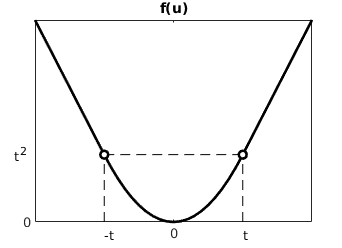
\includegraphics[width=0.5\textwidth]{./figs/norm/huber.png}
        \caption{Huber Penalty}
        \label{fig:huber}
    \end{figure}
    Consider the problem
    \begin{align*}
        \min_{x\in\R^n}\quad J = \sum_{i=0}^{m-1} f(a_i^\tp x - b_i)
    \end{align*}
    \begin{align*}
        \st\quad x\in\poly,
    \end{align*}
    where $f(u)$ is the Huber function
    \begin{align*}
        f(u) &= \left\{\arr{u^2 & \text{if $|u|\leq t$} \\ t(2|u|-t) & \text{else}}\right.,
        \numberthis\label{eqn:huber_penalty}\\
        f'(u) &= \left\{\arr{2u & \text{if $|u|\leq t$} \\ 2t\:\sign(u) & \text{else}}\right.\\
        &=2\:\sat(u,t).
    \end{align*}
    \note{The Huber penalty is a norm.}\\
    This problem is equivalent to \cite[p.~190]{bv_cvxbook}
    \begin{align*}
        \min_{\{x,y,z\}\in\{\R^n,\R^m,\R^m\}}\quad J = y^\tp y+2t\ones^\tp z
    \end{align*}
    \begin{align*}
        \st\quad x&\in\poly,\\
        -y-z&\leq Ax-b\leq y+z,\\
        \zeros\leq y &\leq t\ones,\\
        z&\geq \zeros,
    \end{align*}
    which can be expressed as the \QP
    \begin{align*}
        \min_{\{x,y,z\}\in\{\R^n,\R^m,\R^m\}}\quad J = 
        \frac{1}{2}\mat{x\\y\\z}^\tp
        \mat{
            \zeros^{n\times n} & \zeros^{n\times m} & \zeros^{n\times m} \\ 
            \zeros^{m\times n} & 2\eye_m & \zeros^{m\times m} \\ 
            \zeros^{m\times n} & \zeros^{m\times m} & \zeros^{m\times m}
            }
        \mat{
            x\\y\\z
            }
        +
        \mat{
            \zeros^n \\ \zeros^m \\ 2t\ones^m
            }^\tp
        \mat{
            x\\y\\z
            }
    \end{align*}
    \begin{align*}
        \st\quad x&\in\poly,\\
        \mat{
        \minus A         & -\eye_m         & -\eye_m \\ 
        -A              & -\eye_m         & -\eye_m \\ 
        \minus\zeros^{m\times n}    & \minus\eye_m    & \minus\zeros^{m\times m} \\ 
        \minus\zeros^{m\times n}    & -\eye_m         & \minus\zeros^{m\times m}\\
        \minus\zeros^{m\times n}    & \minus\zeros^{m\times m} & -\eye_m
        }
        \mat{x\\y\\z}
        &\leq
        \mat{
            \minus b\\
            -b\\
            \minus t\ones^m\\ 
            \minus\zeros^m \\ 
            \minus\zeros^m
            }.
    \end{align*}

\clearpage

    \begin{figure}[b]
        \centering
        \subfloat[linear]{{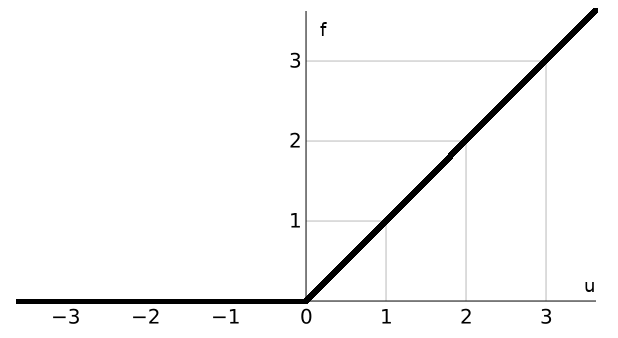
\includegraphics[width=0.42\textwidth]{./figs/norm/relu.png} }}%
        \qquad
        \subfloat[leaky--linear]{{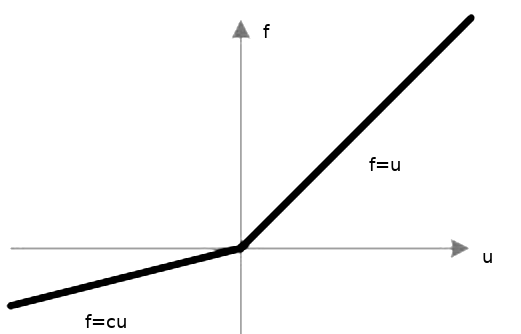
\includegraphics[width=0.4\textwidth]{./figs/norm/leaky_relu.png} }}%
        \caption{Rectified Linear Penalty}%
        \label{fig:relu}%
    \end{figure}

\subsection{Rectified Linear Penalty}

    Consider the problem
    \begin{align*}
        \min_{x\in\R^n}\quad J=\sum_{i=0}^{m-1}f(a_i^\tp x-b_i)
    \end{align*}
    \begin{align*}
        \st\quad x\in\poly,
    \end{align*}
    where $f(u)$ is the rectified linear penalty function
    \begin{align*}
        f(u)&=(u)_+\\
        &=\max(0,u).
    \end{align*}
    This problem can be expressed as the \LP
    \begin{align*}
        \min_{\{x,y\}\in\{\R^n,\R^m\}}\quad J=\ones^\tp y
    \end{align*}
    \begin{align*}
        \st\quad x &\in \poly,\\
        A x - b &\leq y,\\
        0^n &\leq y.
    \end{align*}
    \note{Rectified linear penalty is convex and can be used as a constraint function.}\\
    \note{Rectified linear penalty is the preffered nonlinearity for deep learning \cite{relu}.}

\subsection{Leaky Linear Penalty}
    \begin{align*}
        \min_{x\in\R^n}\quad J=\sum_{i=0}^{m-1}f(a_i^\tp x-b_i)
    \end{align*}
    where $f(u)$ is the leaky--linear penalty function
    \begin{align*}
        f(u)&=(u)_+-t(-u)_+\\
        &=\max(t u,u),
    \end{align*}
    with $t\in\R(0,1)$.
    This problem can be expressed as the \LP
    \begin{align*}
        \min_{\{x,y\}\in\{\R^n,\R^m\}}\quad J= \ones^\tp y
    \end{align*}
    \begin{align*}
        \st\quad x &\in \poly,\\
        A x - b &\leq y,\\
        A x - b &\leq y/t.
    \end{align*}

\clearpage


\section{Duality}

Consider the primal problem

\begin{align*}
    \min_{x\in\R^n}\quad
    J
    &=
            f(x)
\end{align*}
\begin{align*}
    \st\quad A_\ub x&\leq b_\ub,\\
    A_\eq x &= b_\eq.\\
\end{align*}
Let
\begin{align*}
    A = \mat{A_\ub \\ A_\eq},\quad
    b = \mat{b_\ub\\b_\eq}.
\end{align*}


For $A_\ub\in\R^{{r}\times n}$ and $A\in\R^{m\times n}$, the dual problem formulation is

\begin{align*}
    \max_{y\in\R^m}\quad 
    \inf_{x\in\R^n}\quad L(x,y)
\end{align*}
\begin{align*}
    \st\quad  \mat{\eye_{r}&\zeros^{{r}\times (m-{r})}}y\geq \zeros^{r},
\end{align*}

where the Lagrangian is given by

\begin{align*}
    L(x,y) &= f(x)+ y^\tp (A x - b).
\end{align*}

If strong duality holds, the following steps compute $x^*$:
\begin{itemize}
    
    \item Compute $\inf_{x\in\R^n}L(x,y)$ to get $L(x^*,y)$.
    
    \note{This step may not give an explicit representation of $x^*$.}

    Implicit constraints for $L(x^*,y)>-\infty$ can be made explicit.
    
    \item Solve the dual problem to get $y^*$.
    
    \item  The primal problem is solved with $\min_{x\in\R^n}L(x,y^*)$.
    
\end{itemize}

\note{The dual problem may be concave even when the primal problem is not convex.}

\subsection{Norm Duality}

    \begin{figure}[h!]
        \centering
        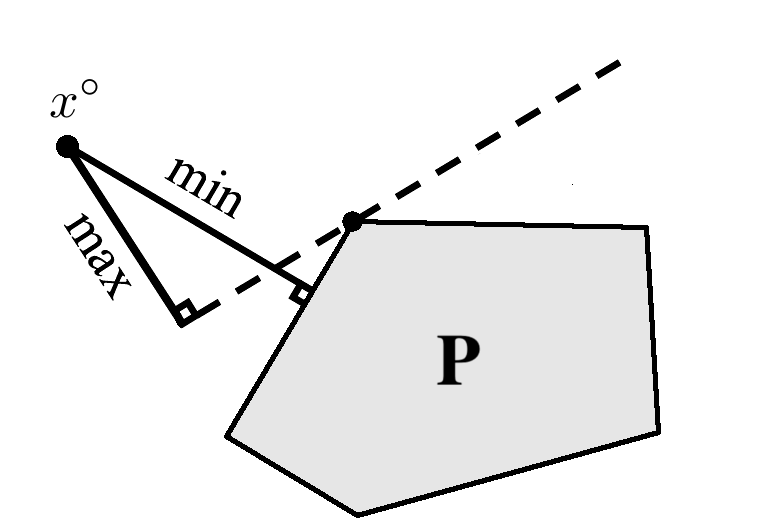
\includegraphics[width=0.35\textwidth]{./figs/dual.png}
        \caption{Norm Duality}
        \label{fig:dual}
    \end{figure}

    Consider the problem

    \begin{align*}
        \min_{x\in\R^n}\quad J = \|x-x^\circ\|
    \end{align*}
    \begin{align*}
        \st \quad x\in\poly.
    \end{align*}
    The dual problem is illustrated in Figure \ref{fig:dual} \cite[p.~9]{luenberger}.

\clearpage

Conisder the problem

\begin{align*}
    \min_{x\in\R^n}\quad J = \|x\|_p
\end{align*}
\begin{align*}
    \st\quad Ax = b.
\end{align*}

The dual problem is given by

\begin{align*}
    \max_{y\in\R^m}\inf_{x\in\R^n}\quad L(x,y) = \|x\|_p + y^\tp (Ax-b),
\end{align*}

which becomes
\cite[p.~221]{bv_cvxbook}\cite[p.~107]{luenberger}\cite[p.~123]{luenberger}

\begin{align*}
    \max_{y\in\R^m}\quad L(x^*,y) = 
    \left\{ 
    \arr{
        -b^\tp y & \text{if}\quad \|A^\tp y\|_q\leq 1\\
        -\infty & \text{else}
    }    
    \right.,
\end{align*}

where $q=p/(p-1)$ for $p\in\R[1,\infty)$.

\note{This does not hold for $p=\infty$.} 

The dual problem can be stated as

\begin{align*}
    \min_{y\in\R^m}\quad -L = b^\tp y
\end{align*}
\begin{align*}
    \st\quad \|A^\tp y\|_q \leq 1.
\end{align*}

\subsubsection{1--Norm}

For $p=1$, $q=\infty$ and this becomes the \LP

\begin{align*}
    \min_{\{y,z\}\in\{\R^m,\R\}}\quad -L = b^\tp y + z
\end{align*}
\begin{align*}
    \st\quad z \leq 1,\\
    -z\ones^n \leq A^\tp y \leq z\ones^n,
\end{align*}
or
\begin{align*}
    \min_{\{y,z\}\in\{\R^m,\R\}}\quad -L =\mat{b\\1}^\tp \mat{y \\ z}
\end{align*}
\begin{align*}
    \st\quad 
    \mat{\minus\zeros^{1\times m} & \minus1\\ \minus A^\tp & -\ones^n \\ -A^\tp & -\ones^n }\mat{y\\z}\leq\mat{1\\\zeros^n\\\zeros^n}.
\end{align*}
\subsubsection{2--Norm}

For $p=2$, $q=2$ and this becomes the \QCQP

\begin{align*}
    \min_{y\in\R^m}\quad -L =b^\tp y
\end{align*}
\begin{align*}
    \st\quad y^\tp Q y \leq 1,
\end{align*}

where $Q=AA^\tp$.  

\clearpage

    \subsection{\LP Duality}
    Consider the primal \LP 
    \begin{align*}
        \min_{x\in\R^n}\quad
        J
        &=
                c^\tp x
    \end{align*}
    \begin{align*}
        \st\quad A_\ub x&\leq b_\ub,\\
        A_\eq x &= b_\eq.\\
    \end{align*}
    Let
    \begin{align*}
        A = \mat{A_\ub \\ A_\eq},\quad
        b = \mat{b_\ub\\b_\eq}.
    \end{align*}


    For $A_\ub\in\R^{{r}\times n}$ and $A\in\R^{m\times n}$, the dual problem formulation is

    \begin{align*}
        \max_{y\in\R^m}\quad 
        \inf_{x\in\R^n}\quad L(x,y)
    \end{align*}
    \begin{align*}
        \st\quad  \mat{\eye_{r}&\zeros^{{r}\times (m-{r})}}y\geq \zeros^{r},
    \end{align*}

    where the Lagrangian is given by

    \begin{align*}
        L(x,y) &= c^\tp x 
        + y^\tp (A x - b)\\
        &= (c^\tp +y^\tp A )x   
        -y^\tp b,
    \end{align*}
    which gives
    \begin{align*}
        L(x^*,y) 
        &= \left\{\arr{-b^\tp y & \text{if $c^\tp +y^\tp A = 0 $}\\
        -\infty & \text{else} }\right..
    \end{align*}

    Making dual constraints explicit gives the \LP

    \begin{align*}
        \min_{y\in\R^m}\quad -L(x^*,y)=b^\tp y
    \end{align*}
    \begin{align*}
        \st\quad  \mat{-\eye_{r}&\zeros^{{r}\times (m-{r})}}y&\leq \zeros^{r},\\
        A^\tp y &=-c.
    \end{align*}

    \subsubsection{Standard Form}
    If the primal problem is in standard form, i.e., $A_\ub = -\eye_n$ and $b_\ub=\zeros^n$,
    the dual can be simplified to \cite[p.~224]{bv_cvxbook}

    \begin{align*}
        \min_{y_\eq\in \R^{m-{r}} }\quad -L\left(x^*,y=\mat{y_\ub\\y_\eq}\right)=b_\eq^\tp y_\eq
    \end{align*}
    \begin{align*}
        \st\quad -A_\eq^\tp y_\eq&\leq c,
    \end{align*}
    where
    \begin{align*}
        y_\ub^*=A_\eq^\tp y_\eq^*+c.
    \end{align*}

\subsection{\QP Duality}

    Consider the primal \QP 

    \begin{align*}
        \min_{x\in\R^n}\quad
        J
        &=\frac{1}{2} x^\tp Q x + c^\tp x
    \end{align*}
    \begin{align*}
        \st\quad A_\ub x&\leq b_\ub,\\
        A_\eq x &= b_\eq.\\
    \end{align*}
    Let
    \begin{align*}
        A = \mat{A_\ub \\ A_\eq},\quad
        b = \mat{b_\ub\\b_\eq}.
    \end{align*}


    For $A_\ub\in\R^{{r}\times n}$ and $A\in\R^{m\times n}$, the dual problem formulation is

    \begin{align*}
        \max_{y\in\R^m}\quad 
        \inf_{x\in\R^n}\quad L(x,y)
    \end{align*}
    \begin{align*}
        \st\quad  \mat{\eye_{r}&\zeros^{{r}\times (m-{r})}}y\geq \zeros^{r},
    \end{align*}

    where the Lagrangian is given by

    \begin{align*}
        L(x,y) &= \frac{1}{2} x^\tp Q x+c^\tp x
        + y^\tp (A x - b)\\
        &= \frac{1}{2} x^\tp Q x+(c^\tp +y^\tp A )x -y^\tp b.
    \end{align*}

\subsubsection{Positive Definite Duality}

    For $Q\in\posdef^n$,

        \begin{align*}
        \pd{L}{x}&=x^\tp Q+  
        c^\tp+y^\tp A.
    \end{align*}
    Setting this to zero and solving gives
    \begin{align*}
        x^*&=-Q^{-1}(A^\tp y+c)
    \end{align*}
    and
    \begin{align*}
        L(x^*,y) &= 
        -\frac{1}{2}(c^\tp +y^\tp A )Q^{-1}(A^\tp y+c) 
        -y^\tp b\\
        &=
        - \frac{1}{2} y^\tp A Q^{-1} A^\tp y
        -
        c^\tp Q^{-1} A^\tp y
        - \frac{1}{2} c^\tp Q^{-1}c
        -
        b^\tp y.
    \end{align*}

    The dual problem is the \QP

    \begin{align*}
        \min_{y\in\R^m}\quad -L(x^*,y)=\frac{1}{2} y^\tp Q_{\text{dual}\:} y + c_{\text{dual}\:}^\tp y
    \end{align*}
    \begin{align*}
        \st\quad  \mat{-\eye_{r}&\zeros^{{r}\times (m-{r})}}y&\leq \zeros^{r},
    \end{align*}
    where
    \begin{align*}
        Q_{\text{dual}\:}&=A Q^{-1} A^\tp,\\
        c_{\text{dual}\:}&=b+A Q^{-1} c.
    \end{align*}

    \note{If $n>m$, the dual problem provides a computationally effecient alternative
    with $m$ free variables to solve.}

\subsubsection{Non--Negative Definite Duality}

    For $Q\in\nonnegdef^n$, SVD gives $Q=\lrs\psv\rrs^\tp$ with $\lrs=\rrs$.  
    Choose 

    \begin{align*}
        x=\mat{\rrs   & \rns }\mat{x_+\\x_0}.
    \end{align*}
    \note{The primal problem can be solved with an ADMM of \LP and positive definite \QP.}\\
    The Lagrangian becomes

    \begin{align*}
        L(x,y) &= \frac{1}{2} x_+^\tp S_+ x_+ +  \mat{c_+^\tp   & c_0^\tp }\mat{x_+\\x_0}  \\
        &\quad+ y^\tp \left( \mat{A_+   & A_0 }\mat{x_+\\x_0} - b_\eq \right)
    \end{align*}
    where
    \begin{align*}
        A_+&:=A\rrs,\quad
        A_0:=A\rns,\\
        c_+^\tp&:=c^\tp\rrs,\quad
        c_0^\tp:=c^\tp\rns.
    \end{align*}
    Minimize $x_+$ with 
    \begin{align*}
        0&=\pd{L}{x_+}\\
        &=x_+^\tp S_++  
        c_+^\tp   +
        y^\tp A_+, 
    \end{align*}
    which gives
    \begin{align*}
        x_+^* =  -S_+^{-1}(A_+^\tp y + c_+).
    \end{align*}
    Minimizing $x_0$,
    \begin{align*}
        L(x^*,y) &= \frac{1}{2} x_+^{*\tp} S_+  x_+^* +  \mat{c_+^\tp   & c_0^\tp }\mat{x_+^*\\x_0}  
        + y^\tp \left( \mat{A_+   & A_0 }\mat{x_+^*\\x_0} - b \right) \\\\
        &=\left\{
            \arr{
                \frac{1}{2} x_+^{*\tp} S_+ x_+^{*}  +\left(   c_+^\tp        
                +   y^\tp A_+ \right) x_+^{*} - b^\tp  y
            & \text{if\quad $c_0
            +A_0^\tp y =\zeros$} \\ 
        -\infty & \text{else}
        }
        \right.\\\\
        &=\left\{
            \arr{
                -\frac{1}{2} x_+^{*\tp} S_+ x_+^{*} - b^\tp  y
            & \text{if\quad $c_0
            +A_0^\tp y =\zeros$} \\ 
        -\infty & \text{else}
        }
        \right.
    \end{align*}

    Making dual constraints explicit gives the \QP

    \begin{align*}
        \min_{y\in\R^m}\quad -L(x^*,y)=\frac{1}{2} y^\tp Q_{\text{dual}\:} y + c_{\text{dual}\:}^\tp y 
    \end{align*}
    \begin{align*}
        \st\quad  \mat{-\eye_{r}&\zeros^{{r}\times (m-{r})}}y&\leq \zeros^{r},\\
        A_0^\tp y&=-c_0,
    \end{align*}
    where
    \begin{align*}
        Q_{\text{dual}\:}&=A_+ S_+^{-1} A_+^\tp,\\
        c_{\text{dual}\:}&=b+A_+ S_+^{-1} c_+.
    \end{align*}

\clearpage

\section{Regularization}

    \begin{figure}[h!]
        \centering
        \subfloat[$p=2,\:q=1$]{{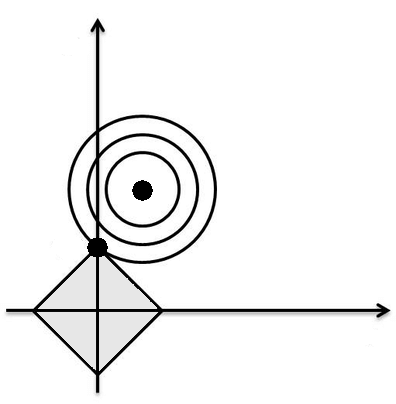
\includegraphics[width=0.2\textwidth]{./figs/reg/lasso_12.png} }}
        \qquad
        \subfloat[$p=\infty,\:q=1$]{{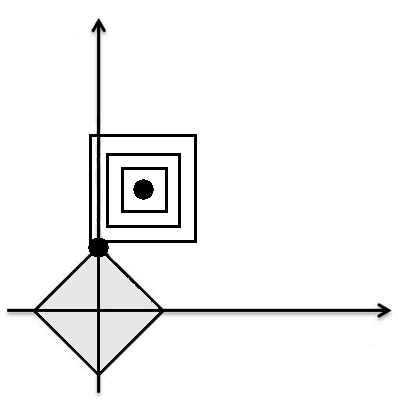
\includegraphics[width=0.2\textwidth]{./figs/reg/lasso_1inf.png} }}
        \qquad
        \subfloat[$p=2,\:q=2$]{{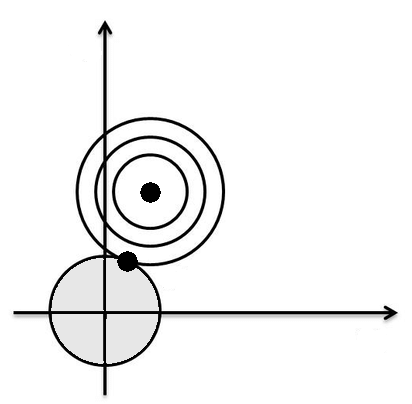
\includegraphics[width=0.2\textwidth]{./figs/reg/lasso_22.png} }}
        \caption{$\ell_p$ residual with $\ell_q$ constraint}%
        \label{fig:lasso}%
    \end{figure}

    % \begin{figure}[b]
    %     \caption{Comparison of contours of $\ell_2$ residual 
    %     with $\ell_1$ constraint v.s. $\ell_2$ constraint.}
    %     \centering
    %     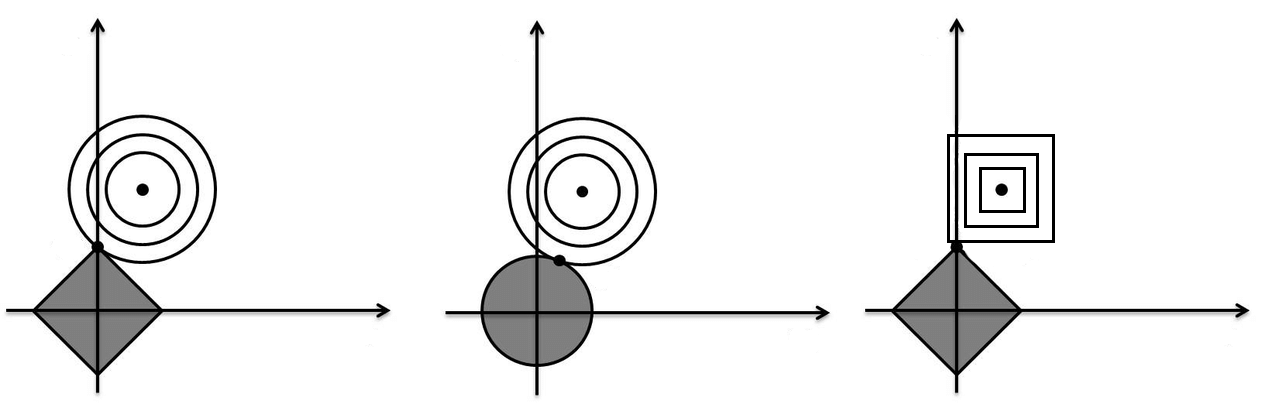
\includegraphics[width=0.4\textwidth]{./figs/lasso.png}
    %     \label{fig:lasso}
    % \end{figure}

    Consider
    \begin{align*}
        \min_{x\in\R^n}\quad J = \|Ax-b\|_p
    \end{align*}
    \begin{align*}
        \st\quad \|x\|_q\leq t,
    \end{align*}

    where $q\in\{1,2,\infty\}$.  The dual problem is \cite{KKT}

    \begin{align*}
        \max_{\lambda\in\R}\min_{x\in\R^n}\quad J = \|Ax-b\|_p+\lambda (\|x\|_q - t)
    \end{align*}
    \begin{align*}
        \st\quad \lambda\geq 0.
    \end{align*}

    The optimal pair $\{x^*,\lambda^*\}$ that meet the threshold $t$ will depend on $\{A,b\}$.  
    Conversely, there exists a $t$ for every fixed selection of $\lambda>0$.  Selecting
    $\lambda>0$, the regularized problem is defined as

    \begin{align*}
        \min_{x\in\R^n}\quad J = \|Ax-b\|_p+\lambda\|x\|_q.
    \end{align*}

    Figure \ref{fig:lasso} shows $\ell_1$ constraints with $\ell_2$ residuals will
    preferentially seek solutions with ordinates at zero. \\
    This also holds true for $\ell_1$ constraints with $\ell_\infty$ residuals, but
    it does not hold true for $\ell_2$ or $\ell_\infty$ constraints.

\subsection{2--Norm Residual with 1--Norm Regularization}

    This is known as LASSO (Least Absolute Shrinkage and Selection Operator).\\ 
    \note{This form of regularization seeks solutions with zeros on the ordinates.}

    The regularized problem is given by
    \begin{align*}
        \min_{x\in\R^n}\quad J
        &=
        \|Ax-b\|_2^2+\lambda\| x\|_1\\
        &=\frac{1}{2} x^\tp Q x + c^\tp x +r + \lambda\|x\|_1,
    \end{align*}
    where
    \begin{align*}
        Q
        &=
            \minus 2A^\tp A,
        \\
            c
        &=
            -2A^\tp b,
        \\
            r
        &=
        \minus b^\tp b,
    \end{align*}
    which can be expressed as the \QP
    \begin{align*}
        \min_{\{x,y\}\in\{\R^n,\R^n\}} \quad 
        J & = \frac{1}{2}
        \left[\begin{array}{c}
            x   \\
            y
        \end{array}\right]^\tp
        \left[\begin{array}{ll}
            Q
        &
            \zeros^{n\times n}
        \\ 
            \zeros^{n\times n}
        &
            \zeros^{n\times n}
        \end{array}\right]
        \left[\begin{array}{c}
            x   \\
            y
        \end{array}\right]
        +
        \left[\begin{array}{l}
            c
            \\
            \ones^{n}
        \end{array}\right]^\tp
        \left[\begin{array}{c}
            x   \\
            y
        \end{array}\right]
    \end{align*}
    \begin{align*}
        \st\quad
        \left[\begin{array}{lll}
                -\lambda\eye_n
            &
                -\eye_n
            \\
                \minus \lambda\eye_n
            &
                -\eye_n
        \end{array}\right]
        \left[\begin{array}{c}
            x   \\
            y
        \end{array}\right]
        &\leq
        \left[\begin{array}{l}
            \zeros^n \\
            \zeros^n
        \end{array}\right].
    \end{align*}

\subsection{Inf--Norm Residual with 1--Norm Regularization}

    \note{This form of regularization seeks solutions with zeros on the ordinates.}
    
    For $A\in\R^{m\times n}$, the regularized problem is given by

    \begin{align*}
        \min_{x\in\R^n} \quad J &= \|Ax-b\|_\infty + \lambda \|x\|_1,
    \end{align*}

    which can be expressed as the \LP

    \begin{align*}
        \min_{\{x,y,z\}\in\{\R^n,\R^n,\R\}} \quad 
        J & = 
        \left[\begin{array}{l}
            \zeros^{n}
            \\
            \ones^{n}
            \\
            1
        \end{array}\right]^\tp
        \left[\begin{array}{c}
            x   \\
            y   \\
            z
        \end{array}\right]
    \end{align*}
    \begin{align*}
        \st\quad 
        \left[\begin{array}{lll}
                -\lambda\eye_n
            &
                -\eye_n
            &
                \minus \zeros^{n}
            \\
                \minus \lambda\eye_n
            &
                -\eye_n
            &
                \minus \zeros^{n}
            \\
                -A
            &
                \minus \zeros^{m\times n}
            &
                -\ones^{m}
            \\
                \minus A
            & 
                \minus \zeros^{m\times n}
            &
                -\ones^{m}
        \end{array}\right]
        &
        \left[\begin{array}{c}
            x   \\
            y   \\
            z
        \end{array}\right]
        \leq
        \left[\begin{array}{l}
            \minus  \zeros^n     \\
            \minus  \zeros^n      \\
            -b           \\
            \minus b
        \end{array}\right].
    \end{align*}

\subsection{2--Norm Residual with 2--Norm Regularization}

    The regularized problem is given by the \QP

    \begin{align*}
        \min_{x\in\R^n}\quad J
        &=
        \|Ax-b\|_2^2+\lambda\| x\|_2^2\\
        &=\frac{1}{2} x^\tp Q x + c^\tp x +b^\tp b,
    \end{align*}

    where

    \begin{align*}
        Q
        &=
            \minus 2A^\tp A+\lambda\eye,
        \\
            c
        &=
            -2A^\tp b.
    \end{align*}

    Computing $A=\lrs\psv\rrs^\tp$ with SVD, 
    the problem can be regularized with uniform circles 
    (as depicted in Figure \ref{fig:lasso}). Using

    \begin{align*}
        x&=\rrs \psv^{-1} y+\rns z,
    \end{align*}

    the reformulation is give by

    \begin{align*}
        \min_{\{y,z\}\in\{\R^r,\R^{n-r}\}}\quad J &= \|\lrs y -  b\|_2^2 + \lambda\|\rrs \psv^{-1} y+\rns z\|_2^2\\
        &= \|y-\lrs^\tp b\|_2^2 + \lambda\|y\|_{2,S_+^{-1}}^2+\lambda \|z\|_2^2 + b^\tp\lns\lns^\tp b\\
        &=\frac{1}{2} \mat{y\\z}^\tp Q \mat{y\\z} + c^\tp \mat{y\\z} +b^\tp b,
    \end{align*}

    where

    \begin{align*}
        Q
        &=
            \mat{\eye_r+\lambda S_+^{-2} & \zeros^{r\times {n-r}} \\
            \zeros^{n-r\times r} & \lambda\eye_{n-r} },
        \\
            c
        &=  \mat{
            -2\lrs^\tp b\\
            \minus \zeros^{n-r}
            }.
    \end{align*}

    \note{The residual is now circular, and the the regularizaton constraint is elliptical and aligned with the axis.}

\clearpage
\subsection{Generalized Regularization}

A more general form of regularization can be given by
\begin{align*}
    \min_{x\in\R^n}\quad J &= \|Ax-b\|+\sum_{i=0}^{n-1}f_i(x_i),
\end{align*}
where $f_i(\cdot)$ is any convex penalty function that can be 
formulated as an \LP or \QP, e.g.,
deadzone or Huber.

\subsection{Non--Convex Regularization}

    For $p\in\R(0,1)$, consider
    \begin{align*}
        \min_{x\in\R^n}\quad J &= \|Ax-b\|_{1/p}+\|x\|_p\\
        &= \left(\sum_{i=0}^{m-1} |a_i^\tp x-b_i|^{1/p}\right)^p
        +\left(\sum_{i=0}^{m-1}|x_i|^p\right)^{1/p}.
    \end{align*}

    This problem formulation gives exceptional sparsity for large $p$.
    It is equivalent to $1/p$--regularized $p$--constrained problem 
    illustrated in Figure \ref{fig:fraction_p_1}.
    This problem is non--convex, which means multiple extremum may occur.
    Figure \ref{fig:fraction_p_2} illustrates non--unique solution.

    The gradient is given by

    \begin{align*}
        \pd{J}{x_j}&=\|r\|_{1/p}^{-1}
        \left(\textstyle\sum_{i=0}^{m-1}|r_i|^{1/p-1}\sign(r_i)A_{ij}\right)
        +\|x\|_p^{-1}|x_j|^{p-1}\sign(x_j),
    \end{align*}
    where
    \begin{align*}
        r_i = a_i^\tp x-b_i,
    \end{align*}
    and the Hessian is given by
    \begin{align*}
        \pdd{J}{x_j}{x_k}&=\frac{p-1}{p}\|r\|_{1/p}^{-2}
        \left(\textstyle\sum_{i=0}^{m-1}A_{ij}\:\sign(r_i)|r_i|^{1/p-1}\right)
        \left(\textstyle\sum_{i=0}^{m-1}A_{ik}\:\sign(r_i)|r_i|^{1/p-1}\right)\\
        &\quad+(1/p-1)\|r\|_{1/p}^{-1}
        \left(\textstyle\sum_{i=0}^{m-1}A_{ij}A_{ik}|r_i|^{1/p-2}\right)\\
        &\quad+p(1/p-1)\|x\|_p^{-2}\sign(x_jx_k)|x_jx_k|^{p-1}\\
        &\quad+(p-1)\|x\|_p^{-1}|x_j|^{p-2}\bin(j=k)
    \end{align*}

    \begin{figure}[b!]
        \centering
        \subfloat[preference for a single axis\label{fig:fraction_p_1}]{{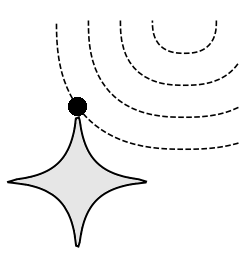
\includegraphics[width=0.25\textwidth]{./figs/reg/fraction_p_1.png} }}
        \qquad
        \subfloat[possible non--unique solutions\label{fig:fraction_p_2}]{{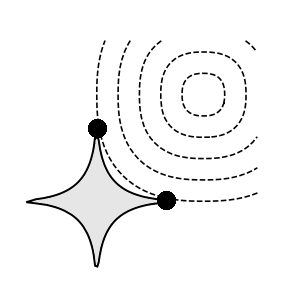
\includegraphics[width=0.25\textwidth]{./figs/reg/fraction_p_2.png} }}
        \caption{non--convex regularization}
    \end{figure}

\clearpage 

\section{Nonlinear Programming}

    Specialized solutions exist for specific forms of nonlinearity, but
    nonlinear programs do not have a general solution.  Convex nonlinear programs
    expressed in standard form can be solved with interior point methods
    with gaurantees on determining feasibility and finding a global minimum.
    Non--convex nonlinear programs may have infinately many local extremum,
    with no gaurantees on determining feasibility or finding a global minimum.
    Nonlinear programs are typically solved by computing local first and second derivatives
    and taking small constrained or regulated steps starting at a random initial guess.
    For the following section, let $d=\|x-x_0\|_2$.

\subsection{Linearizing Nonlinearity Inside Norm}

    Consider the nonlinear function $f(x):\R^n\to\R^m$, and consider

    \begin{align*}
        J &= \|f(x)\|\\
        &= \|f_0+g_0^\tp(x-x_0)+O(d^2)\|\\
        &= \|A_0x+b_0+O(d^2)\|,
    \end{align*}
    where $f_0=f(x_0)$,
    \begin{align*}
        A&= g^\tp,\\
        b&=f-g^\tp x,
    \end{align*}
    and
    \begin{align*}
        g&=\grad f.
    \end{align*}

    If $d^2\leq nr^2$ for a sufficiently small $r>0$, the problem

    \begin{align*}
        \min_{x\in\R^n}\quad J &= \|f(x)\|\\
        \st \quad &x\in\poly
    \end{align*}

    can be solved with Algorithm \ref{algo:itp1} or \ref{algo:itp2}. 
    \note{Any of the penalty functions that result in \LP or \QP can be used.}

    \begin{algorithm}[H]
        \SetAlgoLined
        $x_0 \in\poly$, $r>0$\\
        \While{$x_0$ \emph{not converged}}
        {
            \begin{align*}
                \min_{x\in\R^n}\quad J = \|A_0x+b_0\|
            \end{align*}
            \begin{align*}
                \st \quad &x\in\poly,\\
                -r\ones^n\leq&x-x_0\leq r\ones^n.
            \end{align*}
            $x_0\leftarrow x^*$
        }
    \caption{Nonlinear Solver with Step Bounding Box.
    Alternative: p--norm constraint with Equation [\ref{eqn:p_norm_constraint}].}
    \label{algo:itp1}
    \end{algorithm}
    \begin{algorithm}[H]
        \SetAlgoLined
        $x_0 \in\poly$, $\lambda>0$\\
        \While{$x_0$ \emph{not converged}}
        {
            \begin{align*}
                \min_{x\in\R^n}\quad J = \|A_0x+b_0\|+\lambda\|x-x_0\|
            \end{align*}
            \begin{align*}
                \st \quad &x\in\poly.
            \end{align*}
            $x_0\leftarrow x^*$
        }
    \caption{Nonlinear Solver with Step Regularization}
    \label{algo:itp2}
    \end{algorithm}

\clearpage

\subsection{2--Norm of Nonlinear Function}

    Consider the nonlinear function $f(x):\R^n\to\R^m$. For positive definite $W\in\posdef^m$, consider

    \begin{align*}
        J &= \|f(x)\|_{2,W}^2.
    \end{align*}
    The linear expansion is
    \begin{align*}
        J &= J_0 + g_0^\tp(x-x_0) + O(d^2).
    \end{align*}
    The quadratic expansion is
    \begin{align*}
        J &= J_0 + g_0^\tp(x-x_0)+\frac{1}{2} (x-x_0)^\tp H_0 (x-x_0)+ O(d^3)\\
        &=\frac{1}{2} x^\tp Q_0 x+c_0^\tp x+\text{constant}+ O(d^3),
    \end{align*}
    where
    \begin{align*}
        Q_0&=H_0,\\
        c_0&=g_0-H_0x_0.
    \end{align*}

    If $d^3\leq nr^3$ for a sufficiently small $r>0$, the problem

    \begin{align*}
        \min_{x\in\R^n}\quad J &= \|f(x)\|_{2,W}^2\
    \end{align*}
    \begin{align*}
        \st \quad x\in\poly
    \end{align*}
    can be solved with Algorithm \ref{algo:it21} or \ref{algo:it22}.
    If $\poly=\R^n$, Algorithm \ref{algo:it24} or \ref{algo:it23} can be used.
    \\
    \note{These algorithms can be extended to mixtures of $\ell_p$.}

    \subsubsection{Non--Diagonal Weight}
    For $M=W^\tp W$, the gradient is calculated with
    \begin{align*}
        g^\tp & = \grad J^\tp\\
            & = 2f^\tp M h,
    \end{align*}
    where
    \begin{align*}
        h &= \pd{f}{x},
    \end{align*}
    and the Hessian is calculated with

    \begin{align*}
        H&=\grad^2 J\\
        &= \pd{}{x}\:2h^\tp M f\\
        &=2\:\col\left\{
        \pd{h^\tp}{x_i} M f
        \right\}_{i=0}^{n-1}+2h^\tp M h\\
        &=2\:\col\left\{
            \pd{h^\tp}{x_i} 
            \right\}_{i=0}^{n-1}
        \left(\eye_n\otimes Mf\right)+2h^\tp M h.
    \end{align*}
    Alternatively,
    \begin{align*}
        H&= 
        2(\eye_n \otimes f^\tp M)\pd{\:\mathrm{vec}\left(h^\tp\right)}{x}+2h^\tp M h\\
        &=2\:\row\left\{
            f^\tp M \pd{h}{x_i}
        \right\}_{i=0}^{n-1}+2h^\tp M h.
    \end{align*}
    \note{$H=H^\tp$.}

    \subsubsection{Diagonal Weight}
    If $W=\diag\{w_i\}_{i=0}^{m-1}$
    \begin{align*}
        J = \sum_{i=0}^{m-1} w_i^2 f_i^2.
    \end{align*}
    The gradient is given by
    \begin{align*}
        g&=\grad J \\
        & = \sum_{i=0}^{m-1} 2 w_i^2 f_i \grad f_i
    \end{align*}
    The Hessian is given by
    \begin{align*}
        H&=\pd{}{x}\grad J \\
        &= \sum_{i=0}^{m-1} 2 w_i^2 (\grad f_i \grad f_i^\tp+f_i \grad^2 f_i).
    \end{align*}

\subsubsection{Gradient Search}

    Consider
    \begin{align*}
        \min_{x\in\R^n}\quad J&=J_0 + g_0^\tp(x-x_0)+ O(d^2).
    \end{align*}
    If $\poly=\R^n$, ignoring $O(d^2)$, 
    stepping in the direction of maximum decline with $s\in\R$ 
    and $M\in\posdef^n$,
    \begin{align*}
        x^*(s) &=x_0-2^sMg_0,\\
        J^*(s) &= J_0 -2^s g_0^\tp M g_0+O(2^{2s}).
    \end{align*}
    Algorithm \ref{algo:it24} searches for an optimal $s$ and then takes a scaled step.\\
    \note{$M$ may be normazlied by $\|g_0\|$ or $\|g_0\|^2$ at each iteration.}

\subsubsection{Hessian Search}

    Consider
    \begin{align*}
        \min_{x\in\R^n}\quad J&=J_0 + g_0^\tp(x-x_0)+\frac{1}{2} (x-x_0)^\tp H_0 (x-x_0)+ O(d^3).
    \end{align*}
    If $\poly=\R^n$, ignoring the $O(d^3)$ term, 
    the optimal solution is found by solving
    \begin{align*}
        0 = g_0^\tp + (x^*-x_0)^\tp H_0,
    \end{align*}
    which gives the pure--Newton iteration
    \begin{align*}
        x^*=x_0-H_0^+g_0.
    \end{align*}
    \note{Selecting the matrix condition of the pseudo inverse with SVD can provide a well-conditioned step.}\\
    If the pure--Newton iteration is scaled by $s>0$ with
    \begin{align*}
        x(s)=x_0-sH_0^+g_0,
    \end{align*}
    then,
    \begin{align*}
        J(s) = J_0 +(s^2/2-s)g_0^\tp H_0^+ g_0+O(s^3),
    \end{align*}
    where $(s^2/2-s)$ is negative for $s\in(0,2)$, 
    equal to zero at $s\in\{0,2\}$, 
    and minimum at $s=1$.\\
    Algorithm \ref{algo:it23} searches for an optimal $s$ and then takes a scaled step.


\clearpage

    \begin{algorithm}[H]
        \SetAlgoLined
        $x_0 \in\poly$, $r>0$\\
        \While{$x_0$ \emph{not converged}}
        {
            \begin{align*}
                \min_{x\in\R^n}\quad J = \frac{1}{2}x^\tp Q_0 x+c_0^\tp x 
            \end{align*}
            \begin{align*}
                \st \quad &x\in\poly,\\
                -r\ones^n\leq&x-x_0\leq r\ones^n.
            \end{align*}
            $x_0\leftarrow x^*$
        }
    \caption{Nonlinear $\ell_2$ Solver with Step Bounding Box. 
    Alternative: p--norm constraint with Equation [\ref{eqn:p_norm_constraint}].}
    \label{algo:it21}
    \end{algorithm}
    \begin{algorithm}[H]
        \SetAlgoLined
        $x_0 \in\poly$, $\lambda>0$\\
        \While{$x_0$ \emph{not converged}}
        {
            \begin{align*}
                \min_{x\in\R^n}\quad J = \frac{1}{2}x^\tp Q_0 x+c_0^\tp x +\lambda \|x-x_0\|
            \end{align*}
            \begin{align*}
                \st \quad &x\in\poly.
            \end{align*}
            $x_0\leftarrow x^*$
        }
    \caption{Nonlinear $\ell_2$ Solver with Step Regularization}
    \label{algo:it22}
    \end{algorithm}
    \begin{algorithm}[H]
        \SetAlgoLined
        $x_0\in\poly$, $M\in\posdef^n$\\
        \While{$x_0$ \emph{not converged}}
        {
            \begin{align*}
                x(s)=x_0-2^sMg_0,
            \end{align*}
            \begin{align*}
                \min_{s\in\R} J(x(s)).
            \end{align*}
            $x_0\leftarrow x^*$
        }
    \caption{Unconstrained Nonlinear $\ell_2$ Solver with Gradient Line Search}
    \label{algo:it24}
    \end{algorithm}
    \begin{algorithm}[H]
        \SetAlgoLined
        $x_0\in\poly$\\
        \While{$x_0$ \emph{not converged}}
        {
            \begin{align*}
                x(s)&=x_0-sH_0^+g_0,
            \end{align*}
            \begin{align*}
                \min_{s\in\R(0,2)} J(x(s))
            \end{align*}
            $x_0\leftarrow x^*$
        }
    \caption{Unconstrained Nonlinear $\ell_2$ Solver with Hessian Line Search}
    \label{algo:it23}
    \end{algorithm}
\clearpage
\subsection{Nonlinear Equality Constraints}\label{sec:np_constraint}

    Consider the nonlinear function $f_\eq(x):\R^n\to\R^m$,
    and consider the linear p-norm with nonlinear constraint
    \begin{align}
        \min_{x\in\R^n} \quad J &= \|Ax-b\|\nonumber\\
        \st \quad &x\in\poly,\nonumber\\
        f_\eq(&x)=0.\label{eqn:nonlin_equality}
    \end{align}

\subsubsection{Penalty Approach}

    The nonlinear constraint in Equation \ref{eqn:nonlin_equality} can be brought into the objective function with
    
    \begin{align*}
        \min_{x\in\R^n} \quad J &= \|Ax-b\|+\|f_\eq(x)\|_W
    \end{align*}
    \begin{align*}
        \st \quad &x\in\poly.
    \end{align*}

    \note{The minimum singular value of $W$ must be much larger than 
    the maximum singular value of $A$.}
    \\
    If the residual and regularization are $\ell_2$, then

    \begin{align*}
        \min_{x\in\R^n} \quad J &= \|Ax-b\|_2^2+\|f_\eq(x)\|_{2,W}^2\\
        &=x^\tp A^\tp A x -2 b^\tp Ax +b^\tp b+\|f_{\eq}(x_0)\|_{2,W}^2 + g_0^\tp(x-x_0)+\frac{1}{2} (x-x_0)^\tp H_0 (x-x_0)+ O(d^3)\\
        & = \frac{1}{2} x^\tp Q_0 x +c_0^\tp x +\text{constant} + O(d^3)
    \end{align*}
    \begin{align*}
        \st \quad x&\in\poly,
    \end{align*}
    where
    \begin{align*}
        Q_0&=\minus2A^\tp A + H_0\\
        c_0&=-2A^\tp b+g_0-H_0x_0,
    \end{align*}
    which can be solved with Algorithm \ref{algo:it21} or \ref{algo:it22}.

\subsubsection{Linearization}

    The nonlinear constraint in Equation \ref{eqn:nonlin_equality} can be linearized with
    \begin{align*}
        \min_{x\in\R^n} \quad J = \|Ax-b\|
    \end{align*}
    \begin{align*}
        \st \quad &x\in\poly,\\
        B_{0}&x=c_{0}+O(d^2),
    \end{align*}
    where
    \begin{align*}
        B &= g^\tp,\\
        c &= g^\tp x - f_\eq,
    \end{align*}
    and
    \begin{align*}
        g &= \grad f_\eq.
    \end{align*}
    The constraint $d^2\leq n r^2$ can be added as a box (Algrothim \ref{algo:itc1}),
    p--norm (Algorithm \ref{algo:itc3}), or 
    regularization (Algorithm \ref{algo:itc2}).

    \clearpage

    \begin{algorithm}[H]
        \SetAlgoLined
        $x_0 \in\poly$, $r>0$\\
        \While{$x_0$ \emph{not converged}}
        {
            \begin{align*}
                \min_{x\in\R^n}\quad J = \|Ax-b\|
            \end{align*}
            \begin{align*}
                \st \quad &x\in\poly,\\
                B_{0}\:&x=c_{0}\\
                -r\ones^n\leq&x-x_0\leq r\ones^n.
            \end{align*}
            $x_0\leftarrow x^*$
        }
    \caption{Nonlinear Constrained Solver with Step Bounding Box.}
    \label{algo:itc1}
    \end{algorithm}     
    
    \begin{algorithm}[H]
        \SetAlgoLined
        $x_0 \in\poly$, $r>0$, $p\in\{1,\infty\}$\\
        \While{$x_0$ \emph{not converged}}
        {
            \begin{align*}
                \min_{x\in\R^n}\quad J = \|Ax-b\|
            \end{align*}
            \begin{align*}
                \st \quad &x\in\poly,\\
                B_{0}\:&x=c_{0},\\
                \|&x-x_0\|_p\leq n^{1/p}r.
            \end{align*}
            $x_0\leftarrow x^*$
        }
    \caption{Nonlinear Constrained Solver with p--norm constraint 
    solved with Equation [\ref{eqn:p_norm_constraint}]}
    \label{algo:itc3}
    \end{algorithm} 

    \begin{algorithm}[H]
        \SetAlgoLined
        $x_0 \in\poly$, $\lambda>0$, $a>1$\\
        \While{$\lambda<\lambda^\circ$}
        {
            \While{$x_0$ \emph{not converged}}
            {
                \begin{align*}
                    \min_{x\in\R^n}\quad J = \|Ax-b\|+\lambda\|B_{0}\:x-c_{0}\|
                \end{align*}
                \begin{align*}
                    \st \quad &x\in\poly.
                \end{align*}
                $x_0\leftarrow x^*$
            }
            $\lambda\leftarrow a \lambda$
        } 
    \caption{Nonlinear Constrained Solver with Penalty}
    \label{algo:itc2}
    \end{algorithm}

    \subsubsection{Nonlinear Inequality}

    Consider the nonlinear inequality $f_\ub(x)\leq 0$. 
    A slack variable $y\in\R^m$ can be used to recover nonlinear equality with
    \begin{align*}
        \min_{\{x,y\}\in\{\R^n,\R^m\}} \quad J &= \|Ax-b\|\\
        \st \quad x&\in\poly,\\
        f_\ub(x&)+y =  0,\\
        y&\geq 0.
    \end{align*}

\clearpage

    \subsubsection{Logarithmic Barrier}
    \begin{figure}[h!]
        \centering
        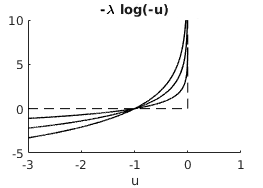
\includegraphics[width=0.35\textwidth]{./figs/np/log_barrier.png}
        \caption{Log--Barrier Penalty}
        \label{fig:log_barrier}
    \end{figure}

    Adding a slack variable, the nonlinar constraint in Equation \ref{eqn:nonlin_equality} can be re--expressed as the nonlinear inequality problem

    \begin{align*}
        \min_{\{x,y\}\in\{\R^n,\R^m\}}\quad J = \|Ax-b\|+\|y\|_W
    \end{align*}
    \begin{align*}
        \st \quad -f_\eq(x)-y&\leq 0,\\
        f_\eq(x)-y&\leq 0.
    \end{align*}
    \note{These constraints force $y\geq0$.}

    For $\lambda>0$, the logrithmic barrier problem is given by \cite[p.~562]{bv_cvxbook}

    \begin{align*}
        \min_{\{x,y\}\in\{\R^n,\R^m\}}\quad J &= \|Ax-b\|+\|y\|_W+\lambda h(x,y),
    \end{align*}
    where 
    \begin{align*}
        h&=-\sum_{i=0}^{m-1}\left(\log(y_i+f_i)+\log(y_i-f_i)\right).
    \end{align*}
    The gradient of $h$ is
    \begin{align*}
        \mat{g_1\\g_2}&=\grad h, 
    \end{align*}
    where
    \begin{align*}
        g_1^\tp&=\pd{h}{x}\\
            &=-\sum_{i=0}^{m-1} \left(\frac{1}{y_i+f_i}-\frac{1}{y_i-f_i}\right)\pd{f_i}{x}, \\\\
        g_2^\tp&=\pd{h}{y}\\
            &=-\sum_{i=0}^{m-1} \left(\frac{1}{y_i+f_i}+\frac{1}{y_i-f_i}\right)\e_i^\tp.
    \end{align*}

    \note{
        This problem formulation is equivalent to the regularized problem

    \begin{align*}
            \min_{x\in \R^n}\quad J = \|Ax-b\|+\|f_\eq(x)\|_W.
    \end{align*}
    }

\clearpage

\subsection{Generalized Reformulations}

There are several generalized problem reformulations.

\subsubsection{Projection}

    Consider nonlinear $f$, $f_\ub$, and $f_\eq$.  
    Any problem can be stated as
    \begin{align*}
        \min_{x\in\R^n}\quad \|f(x)\|
    \end{align*}
    \begin{align*}
        \st\quad x&\in\poly,\\
        f_\ub(x)&\leq b_\ub,\\
        f_\eq(x)&=b_\eq.
    \end{align*}

    Consider a one-to-one projective basis $h(x):\R^n\to\R^m$, and project over the domain $x\in\poly$ to get
    \begin{align*}
        f_{\phantom{\eq}}(x) & \approx A_{\phantom{\eq}} h(x),\\
        f_\ub(x) & \approx A_\ub h(x),\\
        f_\eq(x) & \approx A_\eq h(x),
    \end{align*}
    where
    \begin{align*}
        A_{\phantom{\eq}}&=\left(\int_{x\in\poly} f_{\phantom{\eq}}h^\tp dx\right)\left(\int_{x\in\poly} hh^\tp dx\right)^+,\\
        A_\ub&=\left(\int_{x\in\poly} f_\ub h^\tp dx\right)\left(\int_{x\in\poly} hh^\tp dx\right)^+,\\
        A_\eq&=\left(\int_{x\in\poly} f_\eq h^\tp dx\right)\left(\int_{x\in\poly} hh^\tp dx\right)^+.
    \end{align*}

    The problem can be approximated by
    \begin{align*}
        \min_{y\in\R^m}\quad \|Ay\|
    \end{align*}
    \begin{align*}
        \st\quad y&\in\dom\\
        A_\ub y&\leq b_\ub,\\
        A_\eq y&=b_\eq,
    \end{align*}
    where
    \begin{align*}
        \dom = \{h(x)|x\in\poly\}.
    \end{align*}

    Alternatively, 
    the problem can be approximated by the nonlinear constrained problem

    \begin{align*}
        \min_{\{x,y\}\in\{\R^n,\R^m\}}\quad \|Ay\|
    \end{align*} 
    \begin{align*}
        \st\quad x&\in\poly\\
        A_\ub y&\leq b_\ub,\\
        A_\eq y&=b_\eq,\\ 
        y&=h(x).
    \end{align*}

    The penalty approach can be used to solve this problem.\\

\clearpage

\subsubsection{Epigraph}

    Any problem is equivalent to

    \begin{align*}
        \min_{\{x,y\}\in\{\R^n,\R\}} \quad J =y
    \end{align*}
    \begin{align*}
        \st\quad f(x)-y&\leq0\\
        x&\in\dom.
    \end{align*}

\subsubsection{Indicator Function}

    Any problem is equivalent to

    \begin{align*}
        \min_{x\in\R^n}\quad f(x)
    \end{align*}
    \begin{align*}
        \st\quad \ind(x\in\dom)&\leq0,
    \end{align*}
    
    where

    \begin{align*}
        \ind(x\in\dom)
        &=\left\{ \arr{
            0 & \text{if}\quad x\in\dom\\
            \infty & \text{else}
        }\right..
    \end{align*}

\subsection{Convex Programming}

For $i\in\Z[0,m]$ and convex $f_i(x)$, a general convex problem can be expressed as

\begin{align*}
    \min_{x\in\R^n}\quad J = f_0(x)
\end{align*}
\begin{align*}
    \st \quad f_i(x)&\leq 0,\\
    A x&=b.
\end{align*}

\note{The equality constraint must be linear \cite[p.~137]{bv_cvxbook}.}\\
For $i\in\Z[1,m]$, the constraints define the set

\begin{align*}
    \dom = \{x\in\R^n| f_i(x)\leq 0, Ax =b\}.
\end{align*}

For all $i\in\Z[0,m]$, $x\in\dom$, $y\in\dom$, and $p\in\R[0,1]$, the problem is convex if

\begin{align*}
    f_i(px+(1-p)y)&\leq p f_i(x)+(1-p)f_i(y).
\end{align*}


Any convex problem can be solved with interior point methods.\\
Several convex problems are given special consideration with specialized simplifications and solutions,
e.g.,
\begin{itemize}
    \item \LP: Linear Programs,
    \item \QP: Quadratic Programs,
    \item \SOCP: Second Order Cone Programs \cite[p.~158]{bv_cvxbook},
    \item \QCQP: Quadratic Constrained Quadratic Programs \cite[p.~152]{bv_cvxbook}\cite{sdp},
    \item \GP: Geometric Programs \cite[p.~161]{bv_cvxbook},
    \item \LMI: Linear Matrix Inequalities \cite[p.~169]{bv_cvxbook},
    \item \SDP: Semi Definite Programs \cite[p.~168]{bv_cvxbook}\cite{sdp}.
\end{itemize}
Solvers for each of these specialized convex problems can be found in many programming languages.\\
It is often worth the effort to formulate a problem as one of these standard problems.

\clearpage

\subsubsection{\QCQP: Quadratic Constrained Quadratic Programming}

For $i\in\Z[0,m-1]$, any convex \QCQP can be expressed as 
\begin{align*}
    \min_{x\in\R^n}\quad J = \frac{1}{2} x^\tp Q x + c^\tp x
\end{align*}
\begin{align*}
    \st\quad x\in\poly,\\
    \|A_i x-b_i\|_2^2&\leq 1.
\end{align*}

\note{If $A_i\in\R^{n\times n}$ with $\rank(A_i)=n$, \\
then $\|A_i x-b_i\|_2^2 = \|A_i (x-A_i^{-1}b_i)\|_2^2$ is an ellipse centered at $y_i=A_i^{-1}b_i$ with covariance $(A_i^\tp A_i)^{-1}$.}

A \QCQP can also be expressed as 
\begin{align*}
    \min_{\{x,z_i\}\in\{\R^n,\R^{m_i}\}}\quad J = \frac{1}{2} x^\tp Q x + c^\tp x
\end{align*}
\begin{align*}
    \st\quad x\in\poly,\\
    \|z_i\|_2^2&\leq 1,\\
    A_ix-z_i&=b_i.
\end{align*}

\subsubsection{\SDP: Semi--Definite Programming}

For $A_i\in\sym^n$ and $B\in\sym^n$, the primal \SDP is
\begin{align*}
    \min_{x\in\R^n}\quad J &= c^\tp x\\
    \st\quad \sum_{i=0}^{n-1} x_iA_i &\preceq B.
\end{align*}
This form is also known as an \LMI (linear matrix inequality).

The Lagrangian is
\begin{align*}
    L(x,Y)=c^\tp x +\trace{Y\sum_{i=0}^{n-1}x_iA_i}-\trace{YB},
\end{align*}
with
\begin{align*}
    \inf_{x\in\R^n} L(x,Y)=\left\{\arr{-\trace{BY} & \text{if}\quad \trace{A_iY}+c_i=0\\
    -\infty & \text{else}}\right..
\end{align*}

The dual equals the primal if the primal inequality is strictly feasible.
The dual problem is given by 

\begin{align*}
    \min_{Y\in\R^{n\times n}}\quad J &= \trace{BY}\\
    \st\quad \trace{A_iY}&=-c_i,\\
    Y&\succeq0,
\end{align*}

For $i\in\Z[0,n-1]$, the positive definite constraint 
gives inequality constraints of the form

\begin{align*}
    -\det(M_i)\leq 0,
\end{align*}

where $M_i$ are the principle minors of $Y$, i.e., $M_i=Y[0:i,0:i]$.

If the \SDP is optimized with the interior point method,
\begin{align*}
    \pd{}{Y}\tr(YB)&=B^\tp=B,\\
    \pd{}{Y}\log\det(M_i)&=\tr\left(M_i^{-1}\pd{M_i}{Y}\right).
\end{align*}

\note{If $B\in\sym^n$ and $Y\in\sym^n$, 
$\trace{BY}=\sum_{i=0}^{n-1}\sum_{j=0}^{n-1}B_{ij}Y_{ij}=\vec{B}^\tp\vec{Y}$.}

\note{$x^\tp Q x=\trace{Qxx^\tp}=\trace{QX}$ with $X\succeq0$ and $\rank(X)=1$.}

\clearpage

\subsection{Applications}

Figure \ref{fig:ml} depicts many of the common applications in machine learning.
All of these applications can be framed as optimization problems.
Ideally, optimization should be convex for reliable performance.
Some of these optimization problems can be cast as \LP or \QP,
or they can be solved with iterative \LP or \QP methods.

\begin{figure}[h!]
    \centering
    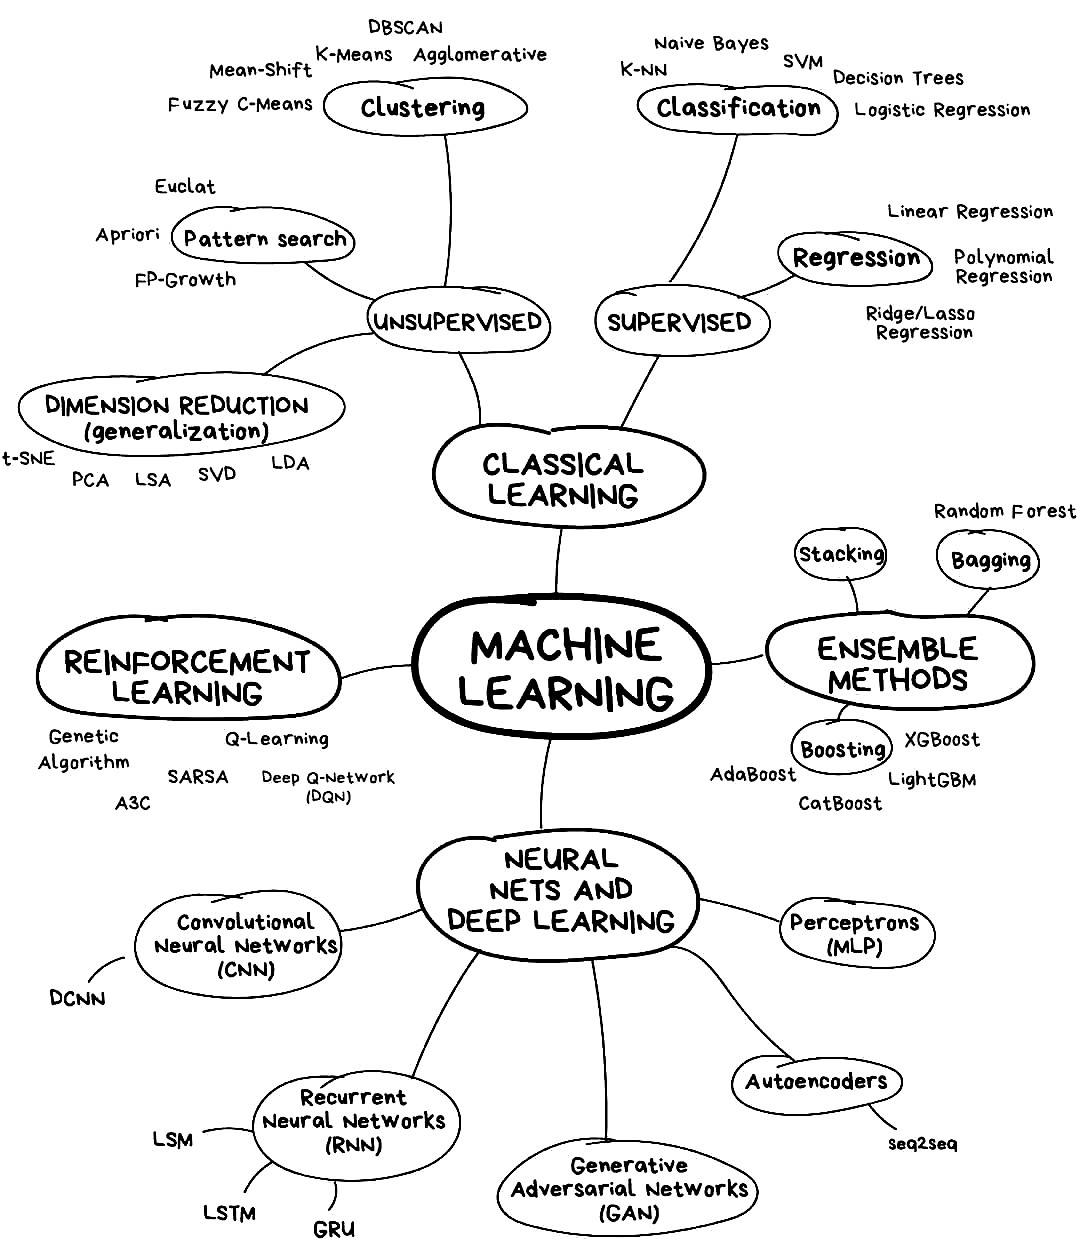
\includegraphics[width=1\textwidth]{./figs/np/ml.jpg}
    \caption{Machine Learning}
    \label{fig:ml}
\end{figure}

\clearpage

\section{Sigmoids}
Sigmoids are a common form of nonlinearity in generalized machine learning applications.\\
Many of them can be expressed as derivatives of the convex penalty functions discussed above.

\subsection{Boolean Sigmoids}

    Boolean sigmoids map $\sig:\R\to\R[0,1]$.
    Figure \ref{fig:relu_sig} shows a sigmoid computed from the gradient of ReLu, and Figure \ref{fig:soft_relu_sig} shows a sigmoid computed from
    the gradient of a right-sidded Huber penalty.
    \begin{figure}[h!]
        \centering
        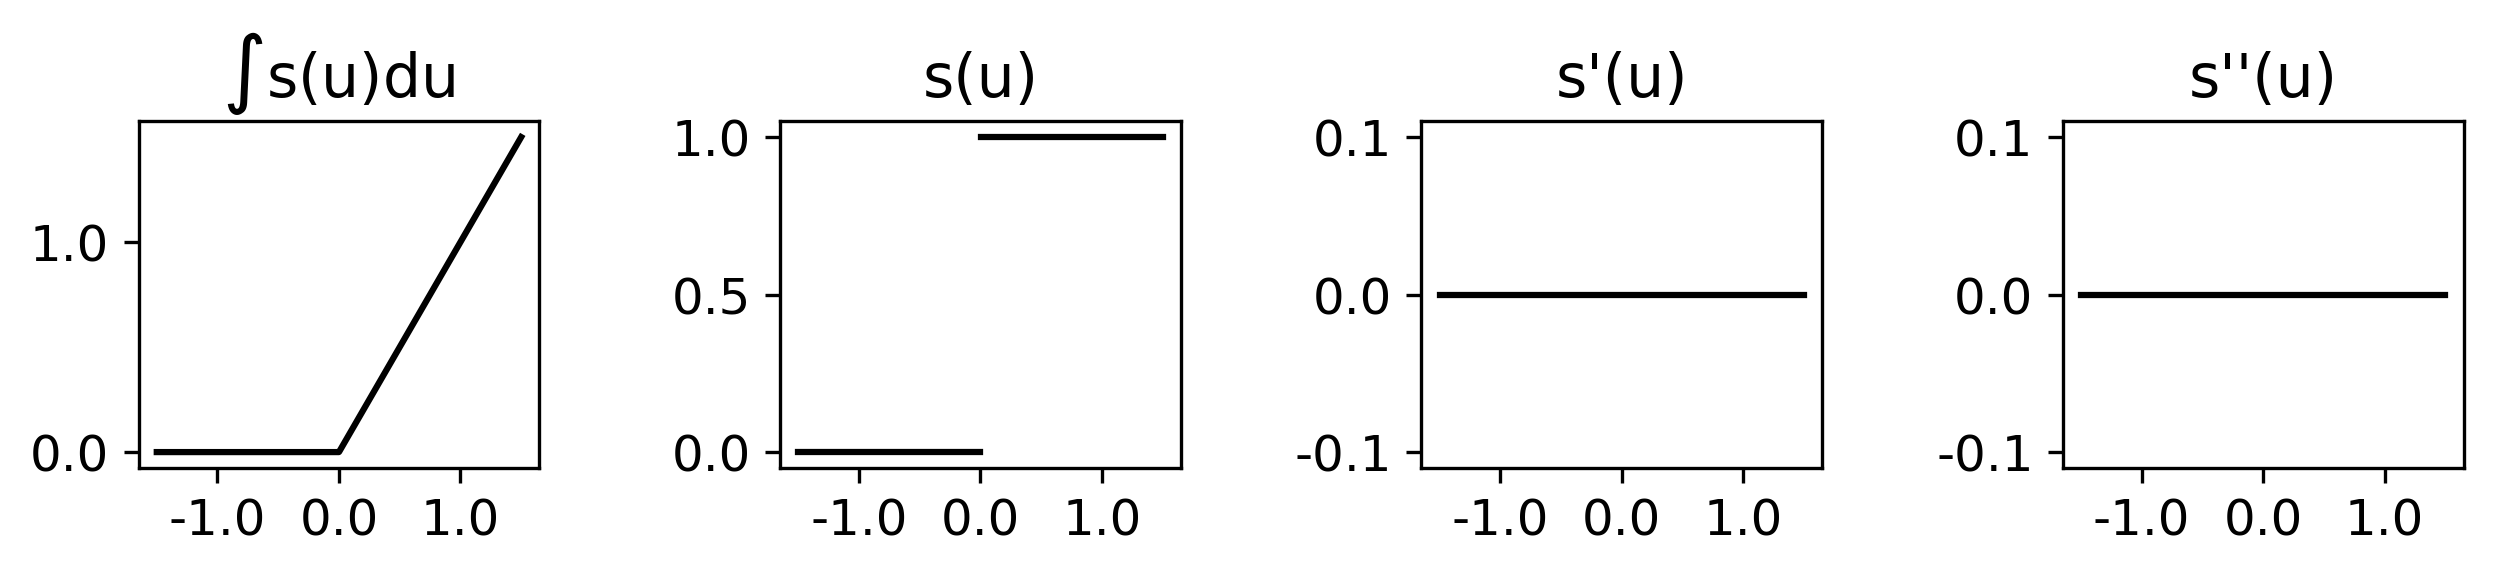
\includegraphics[width=0.75\textwidth]{./figs/nn/sig/relu.png}
        \caption{$\sig(u)=\bin(u>0)$}
        \label{fig:relu_sig}
    \end{figure}
    \begin{figure}[h!]
        \centering
        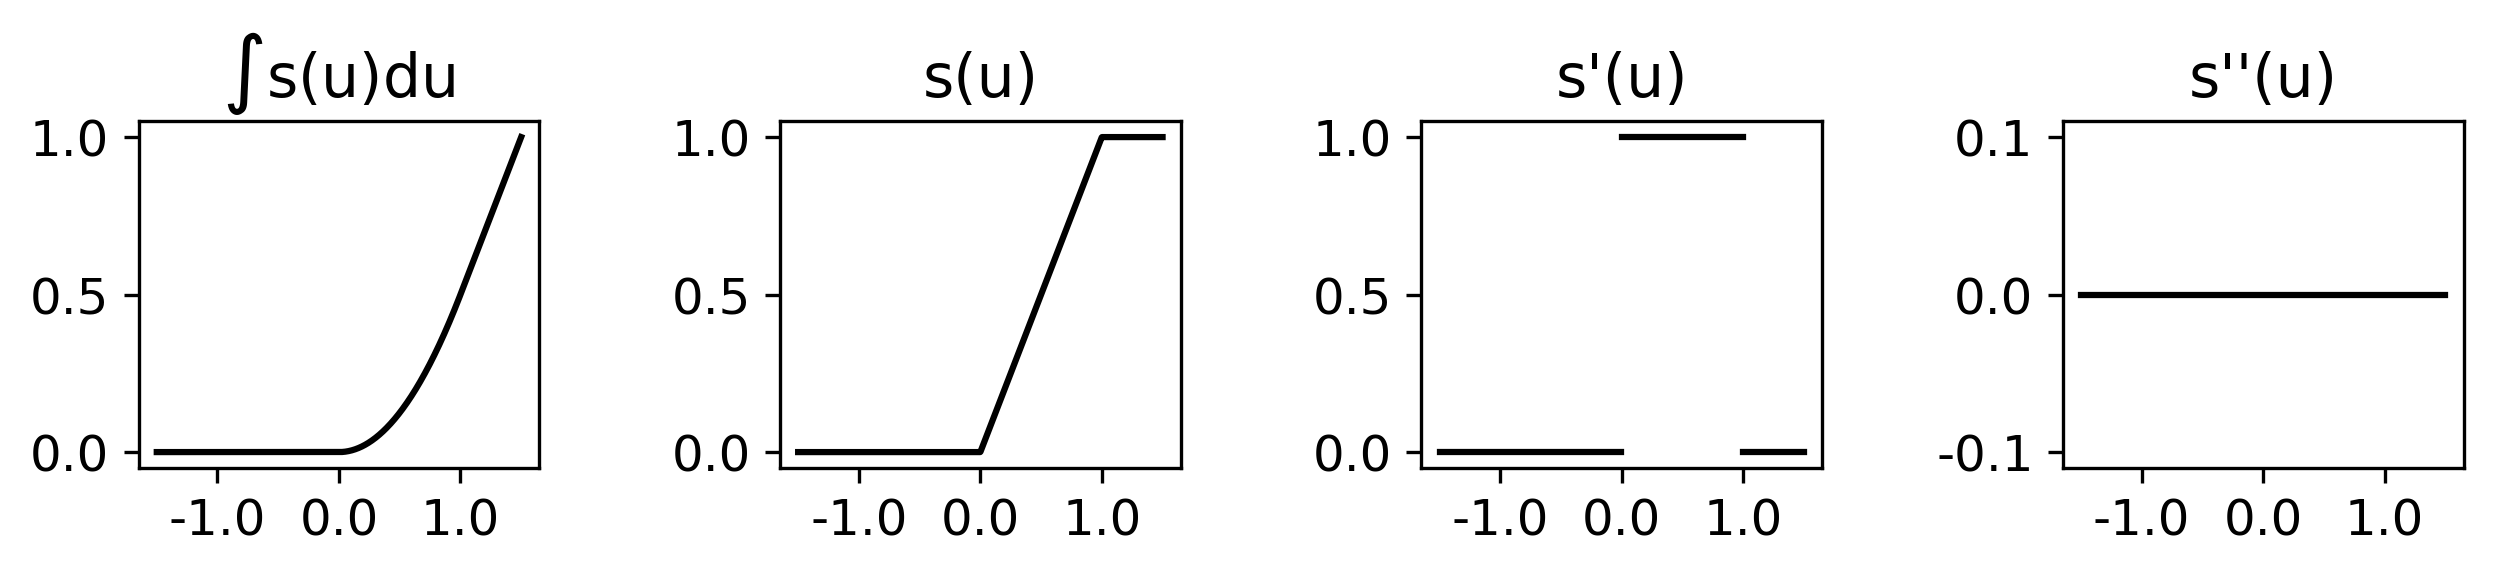
\includegraphics[width=0.75\textwidth]{./figs/nn/sig/soft_relu.png}
        \caption{$\sig(u)=\sat(u,0,1)$}
        \label{fig:soft_relu_sig}
    \end{figure}

    The logistic sigmoid is defined as
    \begin{align*}
        \sig(u) &= (1+e^{-u})^{-1},
    \end{align*}
    with
    \begin{align*}
        \sig'(u)&=\sig(1-\sig),\\
        \sig''(u)&=\sig(1-\sig)^2-\sig^2(1-\sig),\\
        \int s(u) du&= \log(1+e^u).
    \end{align*}
    \note{This function curves primarily for $u\in\R[-2\pi,2\pi]$.}
    \begin{figure}[h!]
        \centering
        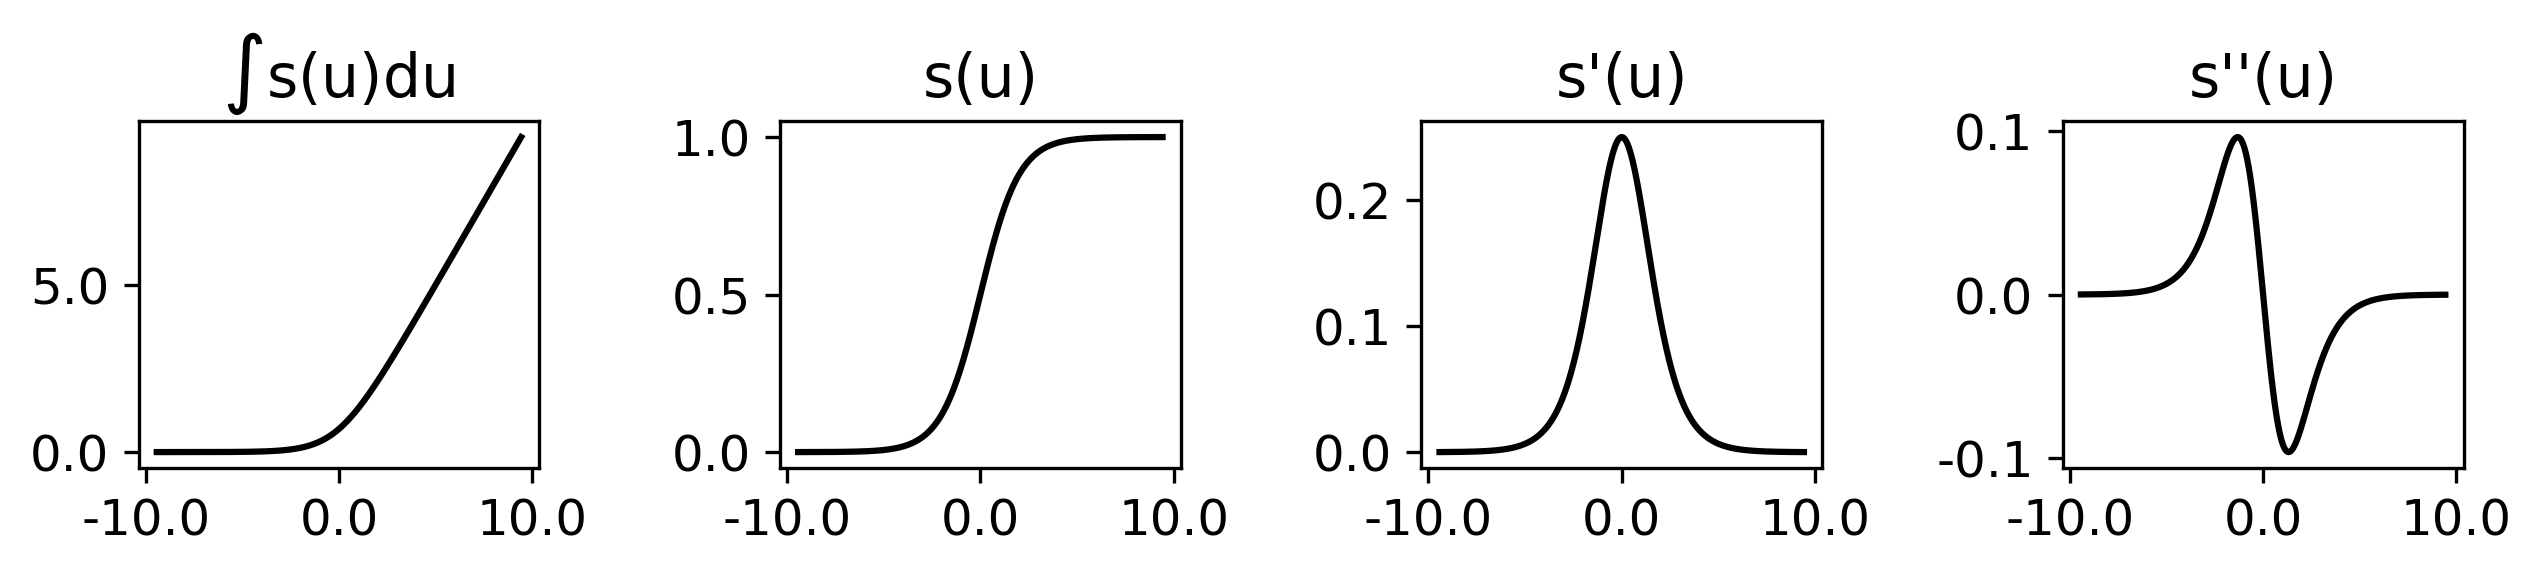
\includegraphics[width=0.75\textwidth]{./figs/nn/sig/logistic.png}
        \caption{$\sig(u)=(1+e^{-u})^{-1}$}
        \label{fig:logistic}
    \end{figure}

    In many applications sigmoid functions that map $\sig:\R\to\R[-1,1]$ are used instead of $\sig:\R\to\R[0,1]$.\\
    It is trivial to re--map in either case.

    \clearpage

\subsection{Piecewise--Polynomial Sigmoids}


There are many ways to obtain an s--shaped curve.  Consider a piecewise polynomial given by
\begin{align*}
    \sig_n(u)=\left\{
        \arr{
            \sum_{i=0}^{2n+1} (a_i/i!)u^i & \text{if}\quad u\in\R[-1,1]
            \\
            \sign(u) & \text{else}
        }\right., 
\end{align*}
where $\sig (-1)=-1$, $\sig (1)=1$, and all derivatives at $u\in\{-1,1\}$ are zero.
For $n\in\Z[0,3]$ and $|u|<1$, this gives
\begin{align*}
    \sig_0(u)&=u,\\
    \sig_1(u)&=(3 u - u^3)/2,\\
    \sig_2(u)&=(15 u - 10 u^3 + 3 u^5)/8,\\
    \sig_3(u)&=(35 u - 35 u^3 + 21 u^5 - 5 u^7)/16,
\end{align*}
Figures \ref{fig:poly0}--\ref{fig:poly3} show $n\in\Z[0,3]$.\\
\note{The Huber penalty function at $t=1$ is given by $f_0=\int s_0(u)du$.}

\begin{figure}[h!]
    \centering
    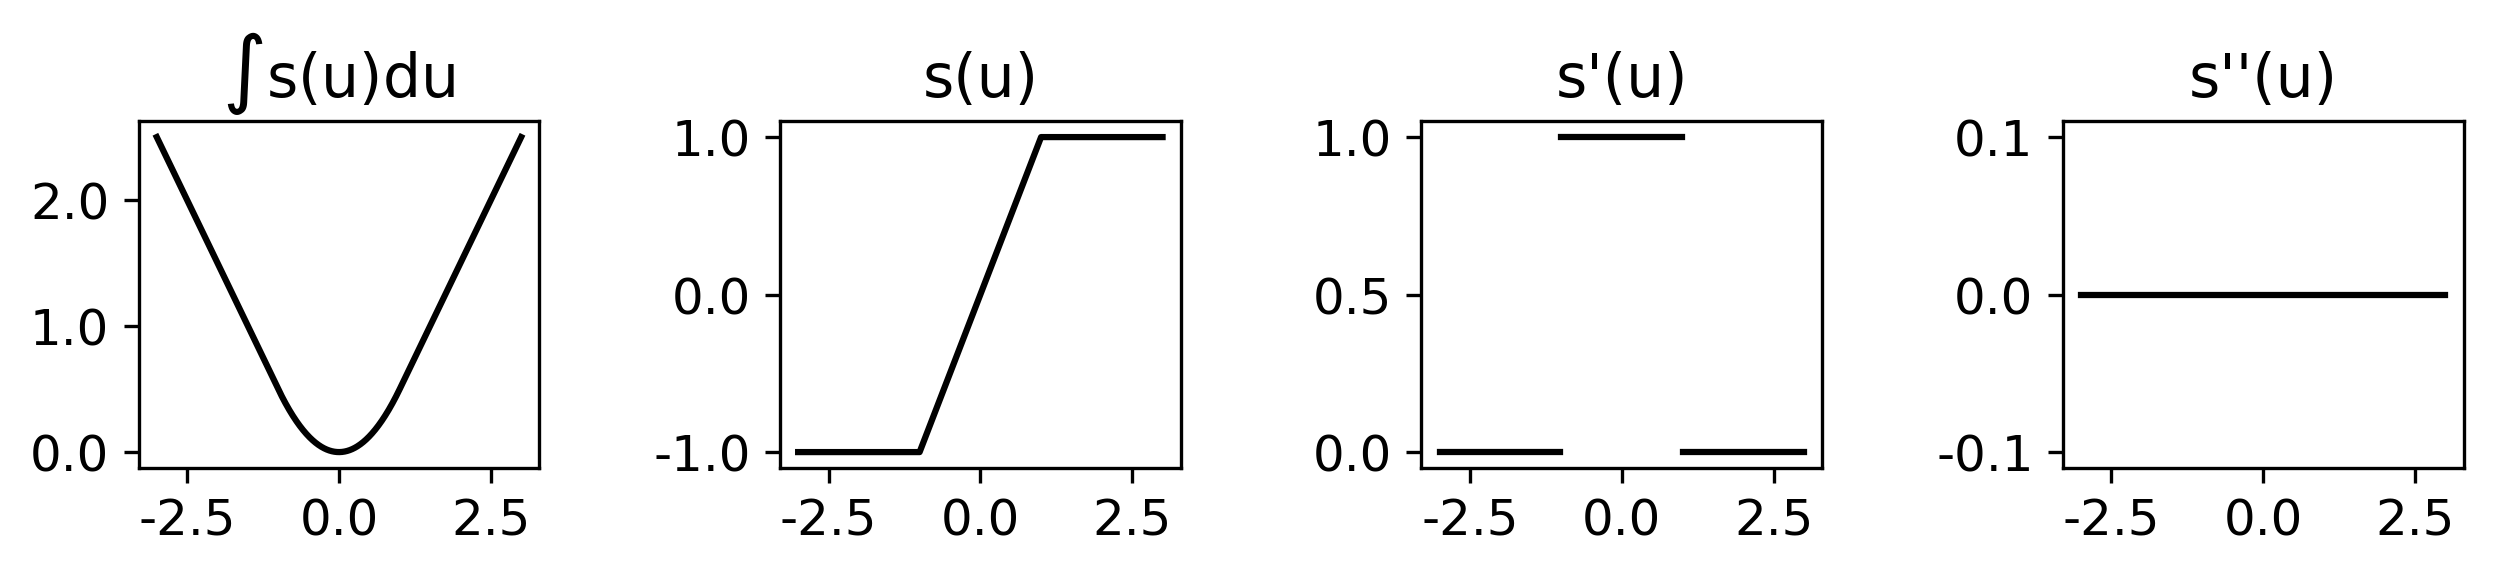
\includegraphics[width=0.7\textwidth]{./figs/nn/sig/poly0.png}
    \caption{$\sig_0(u)=\sat(u)$}
    \label{fig:poly0}
\end{figure}
\begin{figure}[h!]
    \centering
    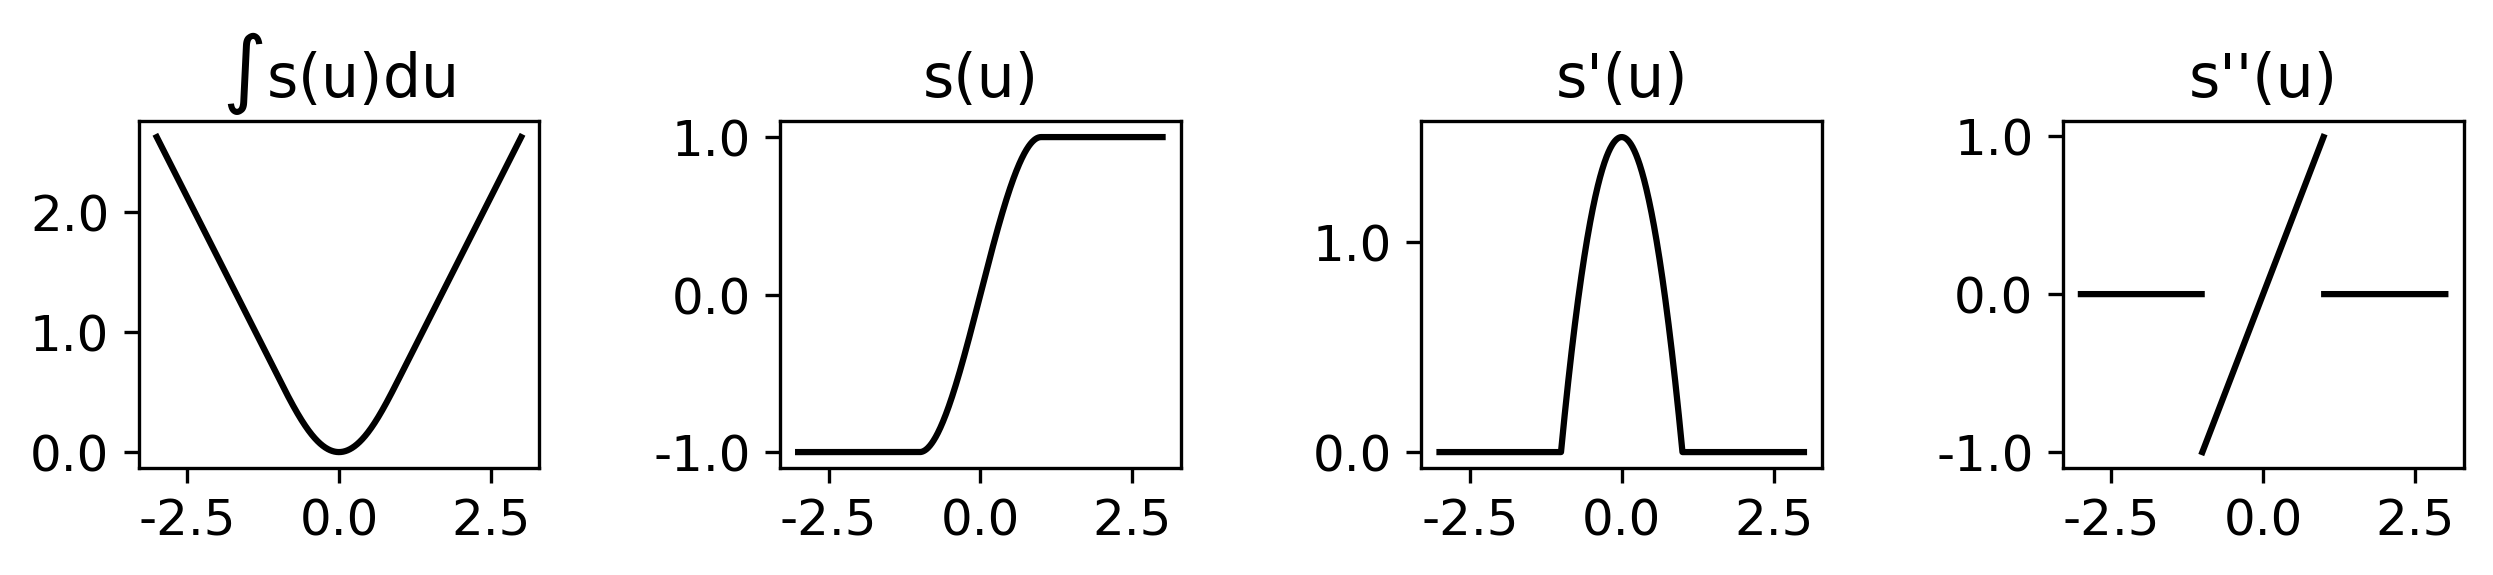
\includegraphics[width=0.7\textwidth]{./figs/nn/sig/poly1.png}
    \caption{$\sig_1(u)$}
    \label{fig:poly1}
\end{figure}
\begin{figure}[h!]
    \centering
    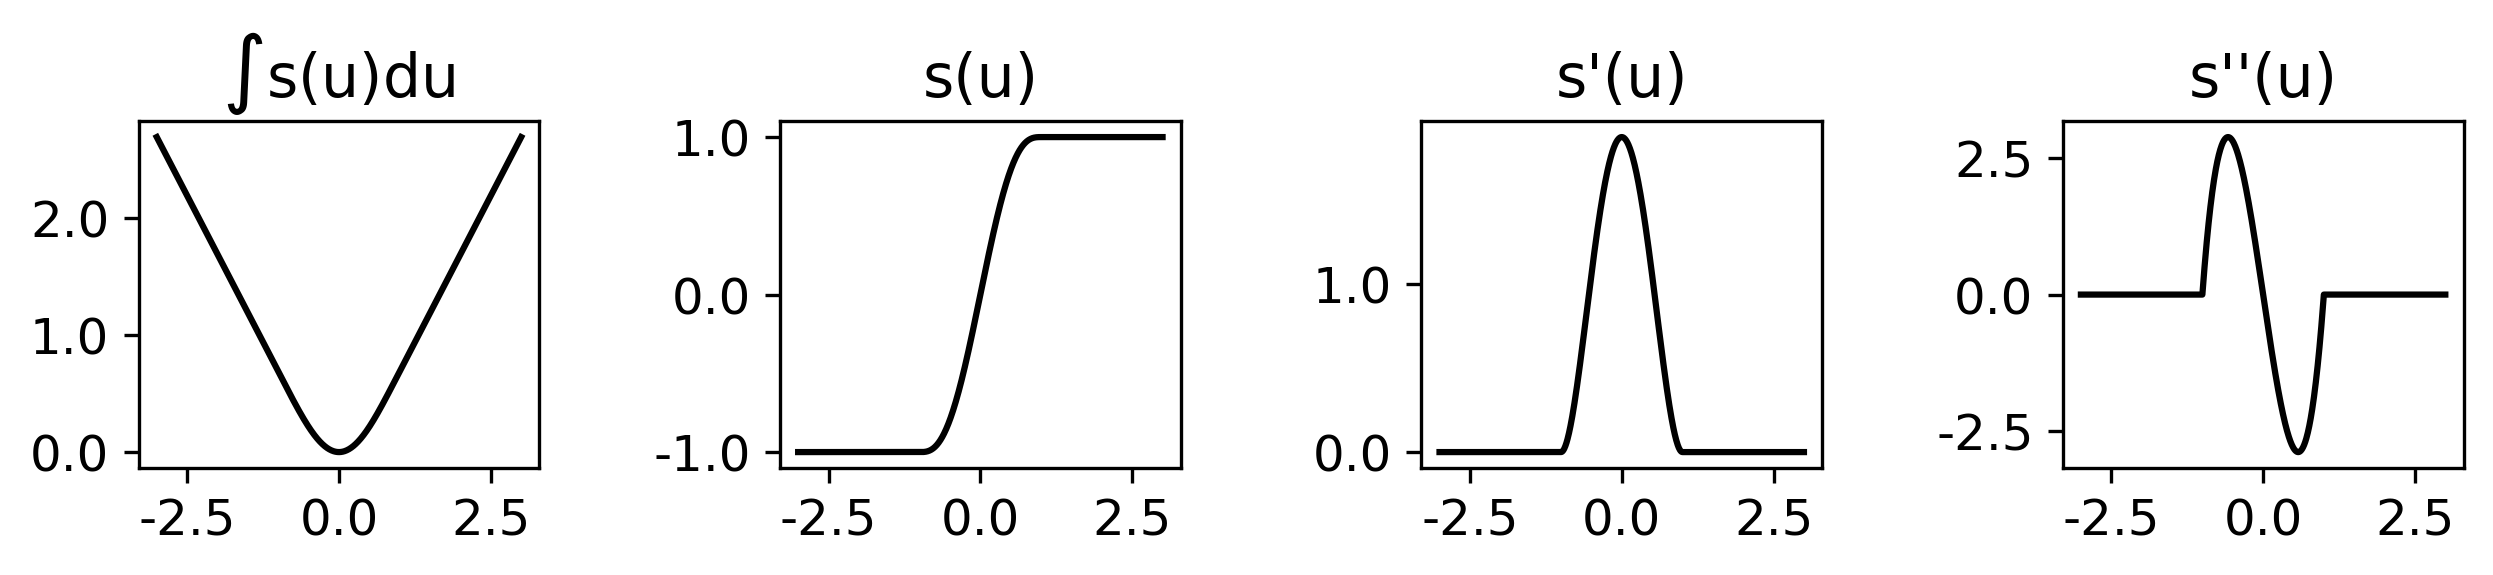
\includegraphics[width=0.7\textwidth]{./figs/nn/sig/poly2.png}
    \caption{$\sig_2(u)$}
    \label{fig:poly2}
\end{figure}
\begin{figure}[h!]
    \centering
    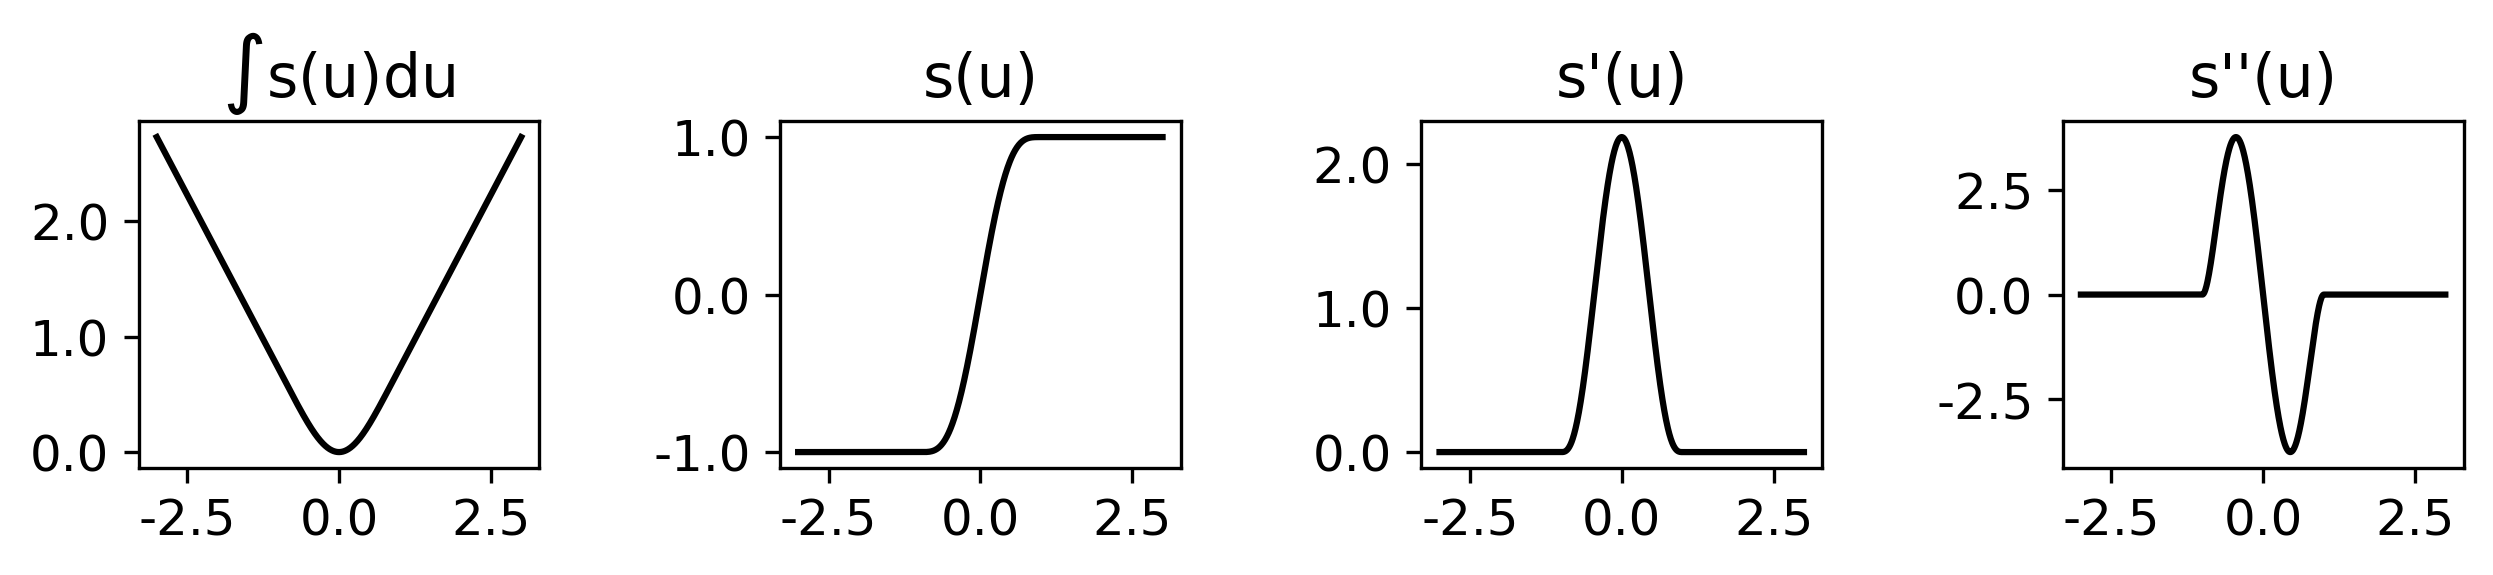
\includegraphics[width=0.7\textwidth]{./figs/nn/sig/poly3.png}
    \caption{$\sig_3(u)$}
    \label{fig:poly3}
\end{figure}


\clearpage
    Dividing $f_i=\int s_i(u)du$ by $u$ gives alternative sigmoid functions. For $|u|<1$,
    \begin{align*}
        f_0/u&=u/2,\\
        f_1/u&=\left(6u-u^3\right)/8,\\
        f_2/u&=\left(15u-5u^3+u^5\right)/16,\\
        f_3/u&=\left(140u-70u^3+28u^5-5u^7\right)/128.
    \end{align*}
    For $|u|>1$,
    \begin{align*}
        \frac{f_i}{u}&=\sign(u)+\frac{f_i(1)-1}{u}.
    \end{align*}
    The gradient approaches zero asymptotically.
    Figures \ref{fig:inv_poly0}--\ref{fig:inv_poly3} show $n\in\Z[0,3]$.
    \begin{figure}[h!]
        \centering
        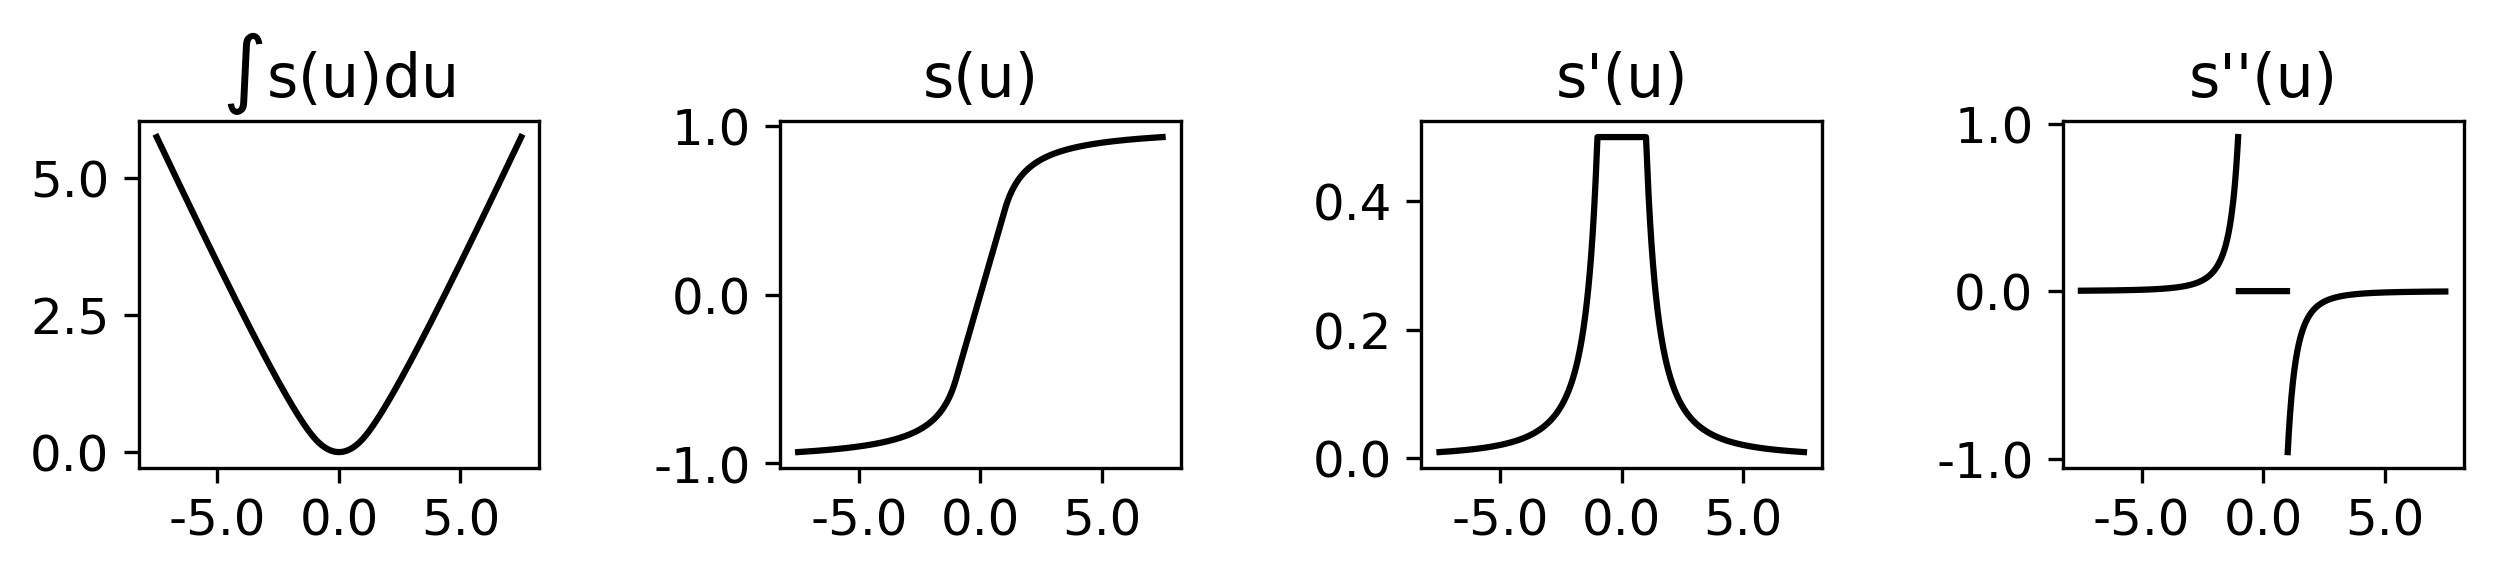
\includegraphics[width=0.7\textwidth]{./figs/nn/sig/inv_poly0.png}
        \caption{$s_0(u)\leftarrow f_0(u)/u$}
        \label{fig:inv_poly0}
    \end{figure}
    \begin{figure}[h!]
        \centering
        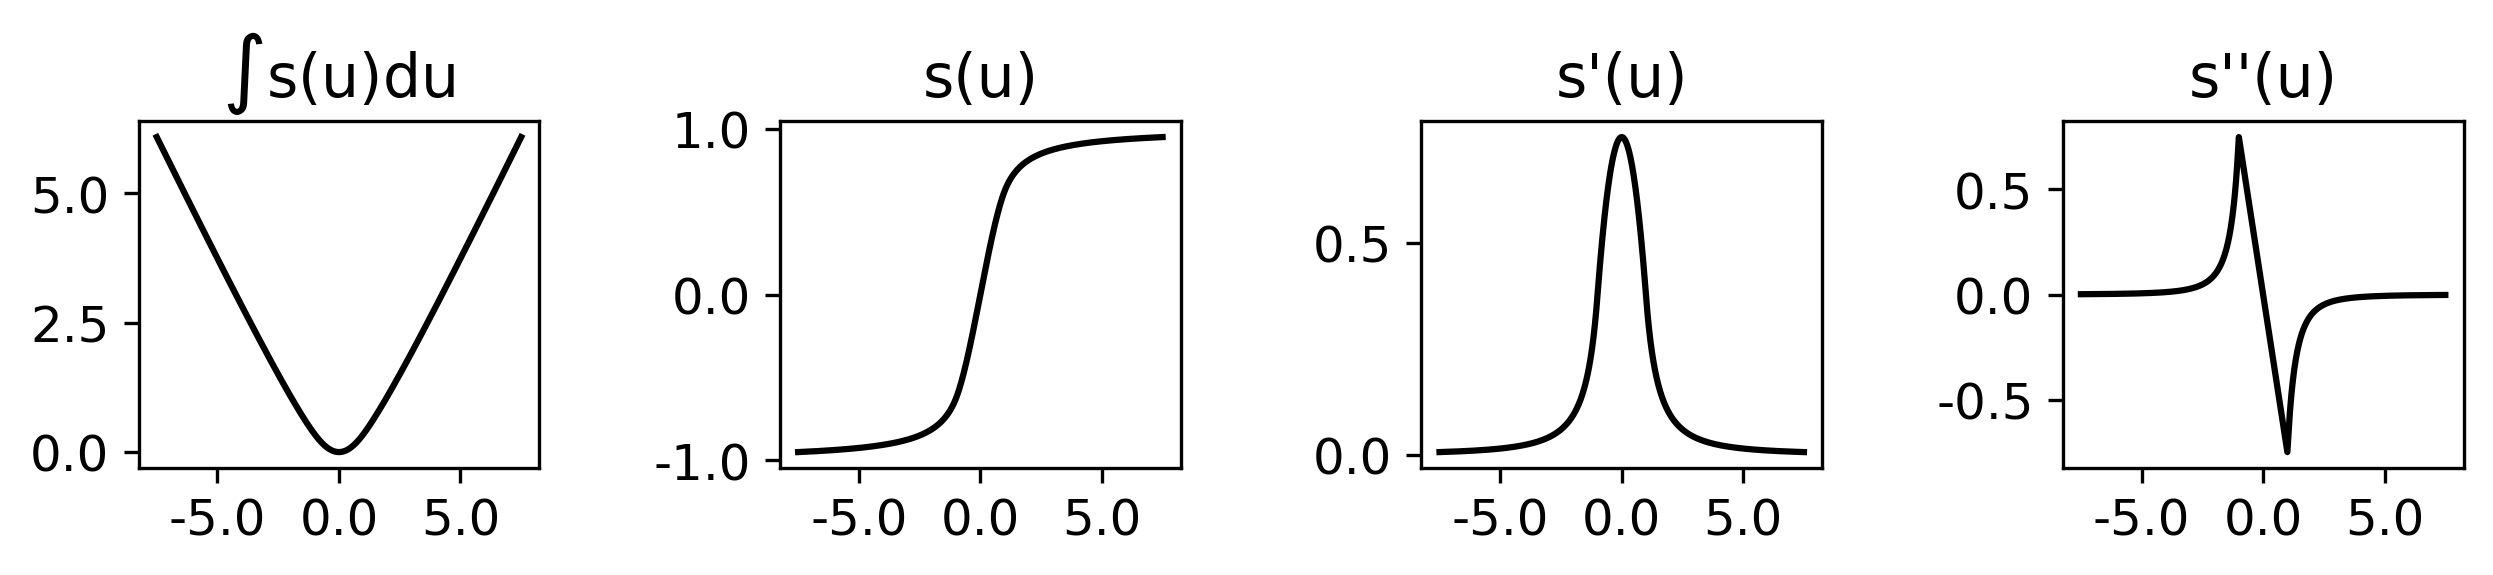
\includegraphics[width=0.7\textwidth]{./figs/nn/sig/inv_poly1.png}
        \caption{$s_1(u)\leftarrow f_1(u)/u$}
        \label{fig:inv_poly1}
    \end{figure}
    \begin{figure}[h!]
        \centering
        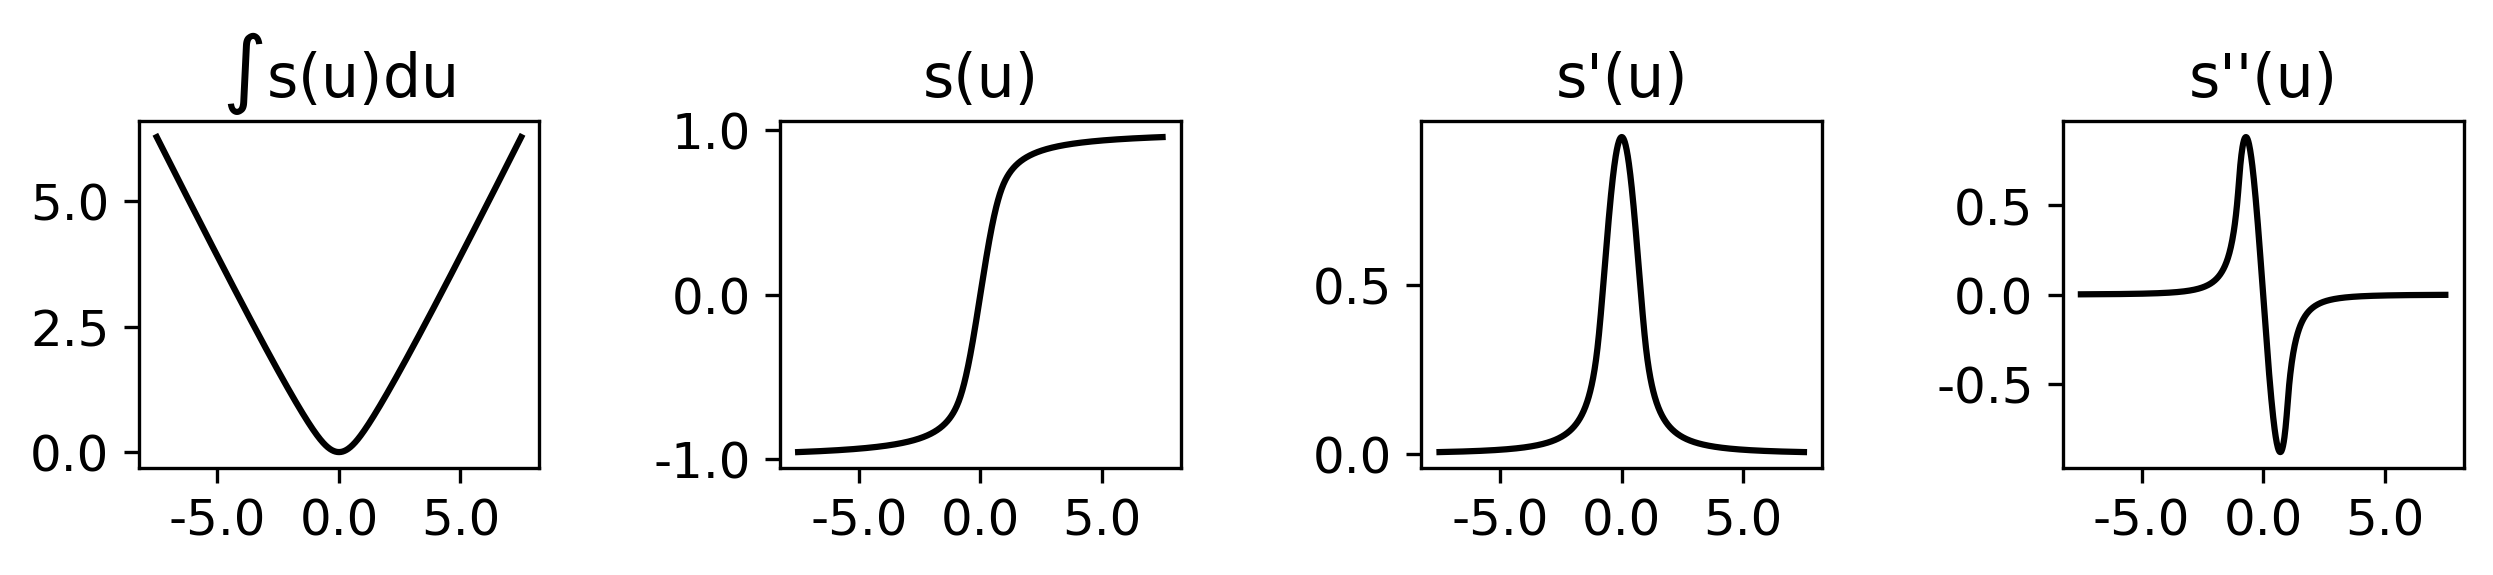
\includegraphics[width=0.7\textwidth]{./figs/nn/sig/inv_poly2.png}
        \caption{$s_2(u)\leftarrow f_2(u)/u$}
        \label{fig:inv_poly2}
    \end{figure}
    \begin{figure}[h!]
        \centering
        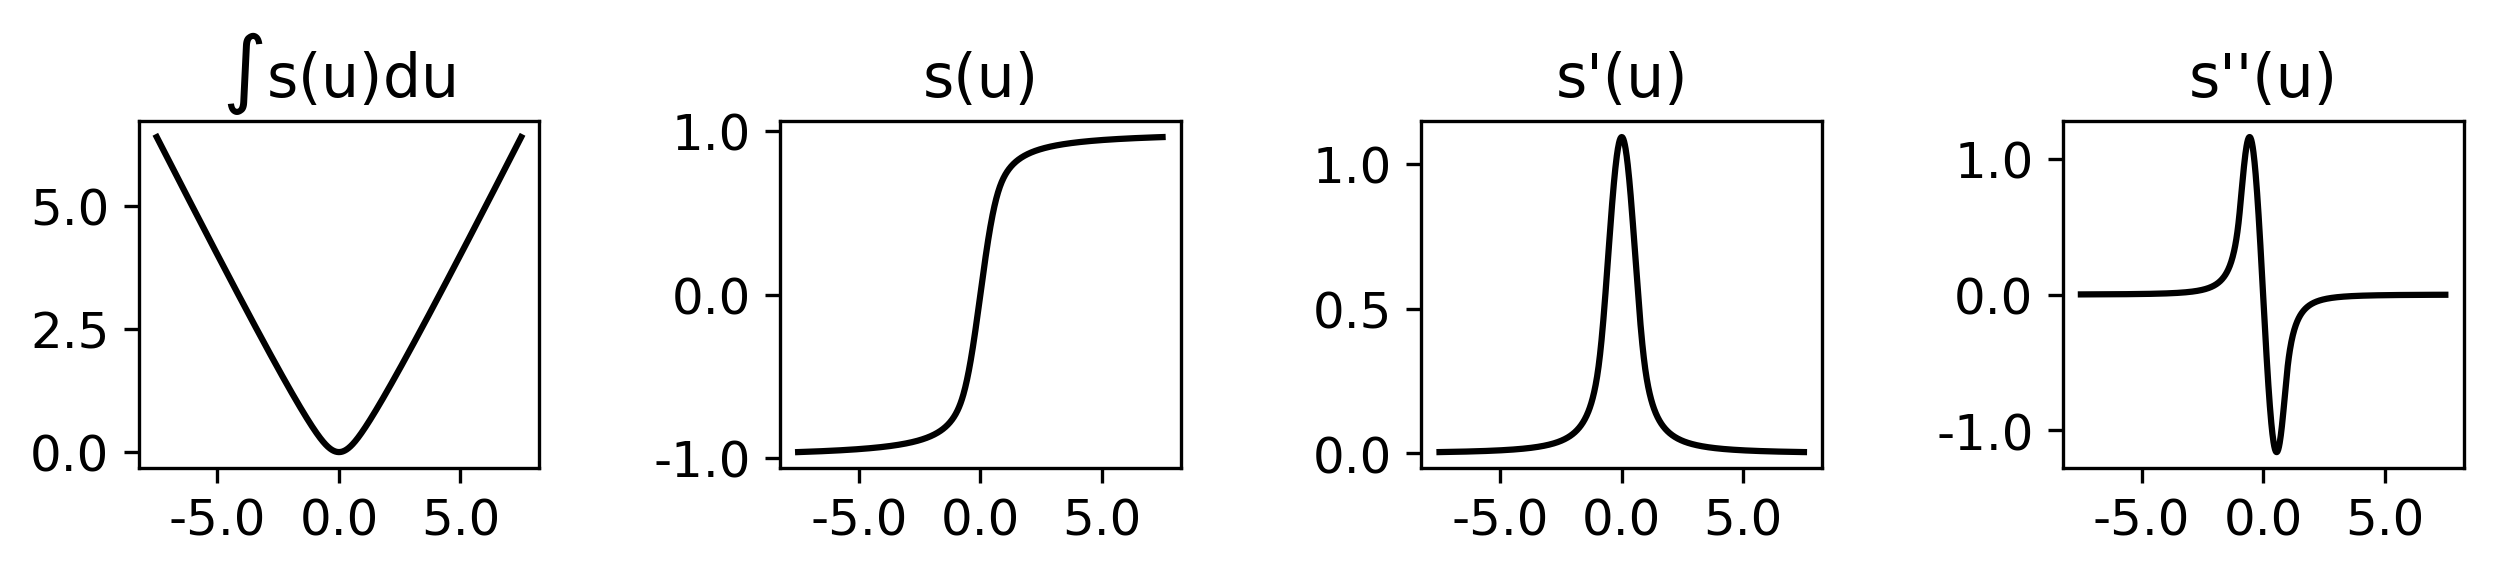
\includegraphics[width=0.7\textwidth]{./figs/nn/sig/inv_poly3.png}
        \caption{$s_3(u)\leftarrow f_3(u)/u$}
        \label{fig:inv_poly3}
    \end{figure}

    \note{For $r_i=a_i^\tp x - b_i$,
    \begin{align*}
        \|Ax-b\|_1&\approx
        \textstyle\sum_{i=0}^{m-1} r_i\sig(r_i),\\
        \pd{}{x}\|Ax-b\|_1&\approx
        \textstyle\sum_{i=0}^{m-1} (s(r_i) + r_is'(r_i))a_i^\tp.
    \end{align*}
    }
    \clearpage

    \subsection{Deadzone Sigmoid}
        For the deadzone penalty $f(u)$, consider the sigmoid function given by
        \begin{align*}
            \sig(u)&=\frac{f(u)}{u}\\
            &=
            \left\{\arr{0 & \text{if $|u|\leq t$} \\ \sign(u)-t/u & \text{else}}\right..
        \end{align*}
        Figure \ref{fig:deadzone_sigmoid} plots the sigmoid curve. 
        \note{In the limit of $|u|\to\infty$, the sigmoid approaches $\sign(u)$ asymptotically.} 
        \\
        \note{The asymptotic approach is much slower than a logistic sigmoid.}\\
        A constraint of the form
        \begin{align*}
            y=\sig(u)
        \end{align*}
        can be expressed as
        \begin{align*}
            yu=
            \left\{\arr{0 & \text{if $|u|\leq t$} \\ |u|-t & \text{else}}\right.\quad\text{or}\quad
            (yu+t)^2=
            \left\{\arr{t^2 & \text{if $|u|\leq t$} \\ u^2 & \text{else}}\right.
            .
        \end{align*}
        The first derivative is
        \begin{align*}
            \sig'(u)
            &=
            \left\{\arr{0 & \text{if $|u|\leq t$} \\ t/u^2 & \text{else}}\right.,
        \end{align*}
        and the second derivative is
        \begin{align*}
            \sig''(u)
            &=
            \left\{\arr{0 & \text{if $|u|\leq t$} \\ -2t/u^3 & \text{else}}\right..
        \end{align*}
        \note{When $t=0$, $\sig(u)=\sign(u)$ and the constraint can be expressed as $yu=|u|=\max(-u,u)$.}
        \begin{figure}[h!]
            \centering
            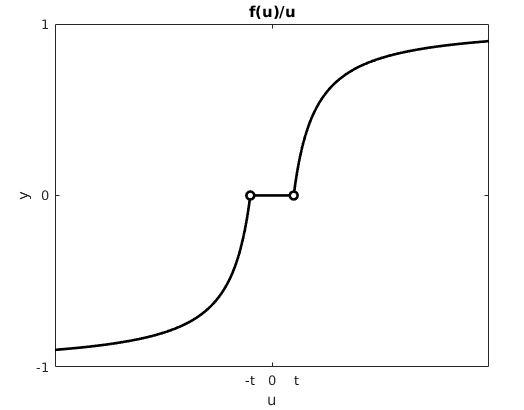
\includegraphics[width=0.5\textwidth]{./figs/nn/deadzone_sigmoid.png}
            \caption{Deadzone Sigmoid}
            \label{fig:deadzone_sigmoid}
        \end{figure}
        \begin{figure}[h!]
            \centering
            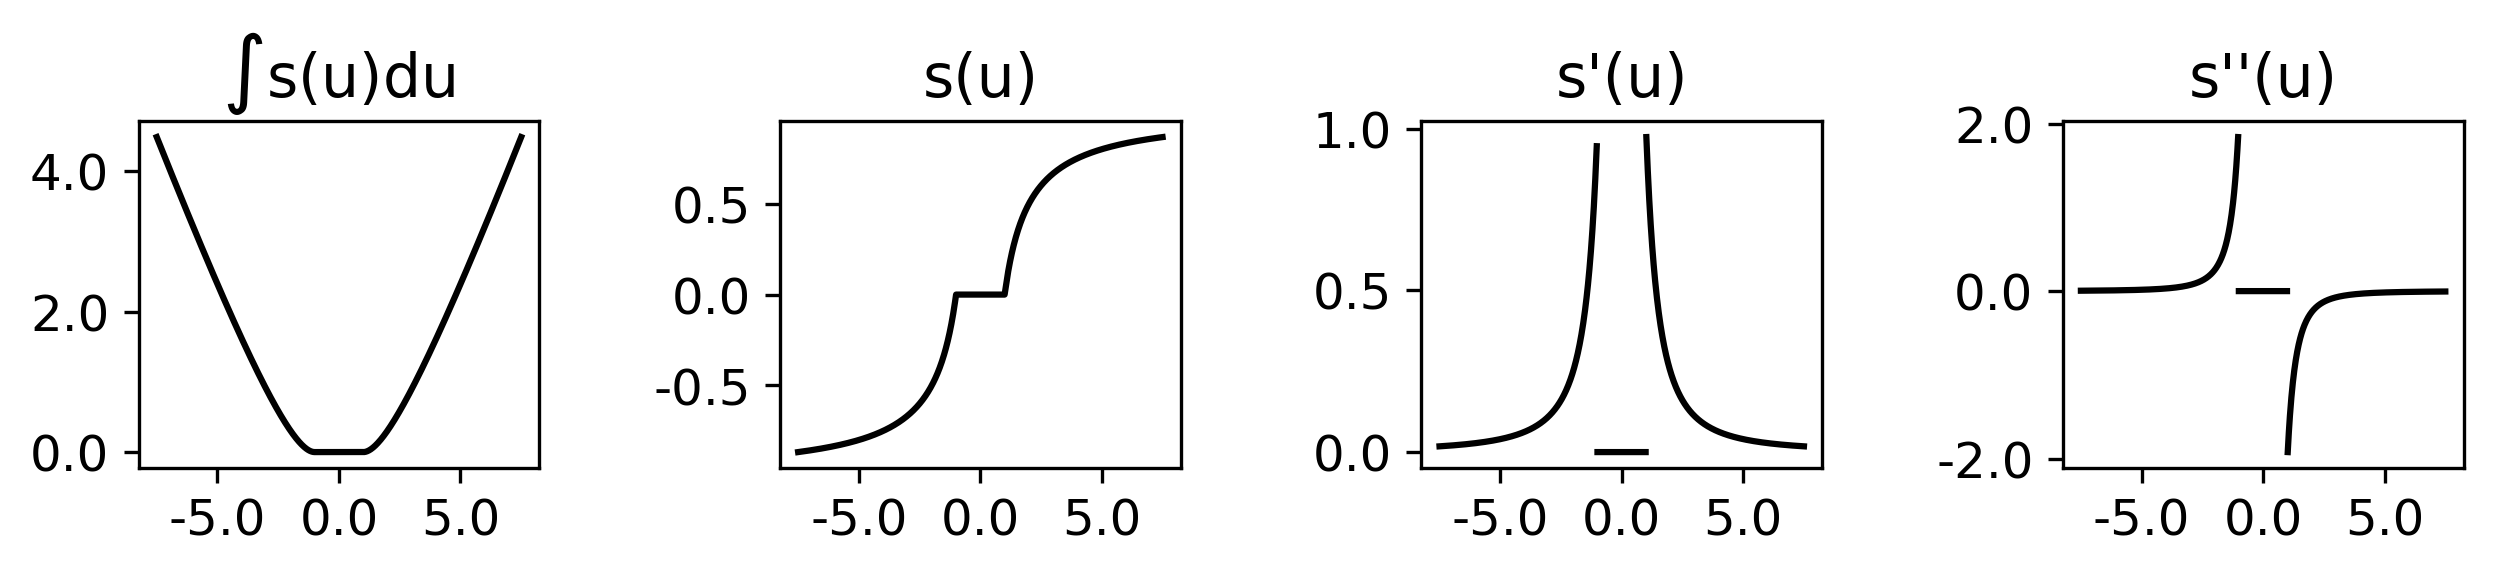
\includegraphics[width=0.7\textwidth]{./figs/nn/sig/deadzone.png}
            \caption{Deadzone Sigmoid}
            \label{fig:sig_deadzone}
        \end{figure}

\subsection{Huber Sigmoid}
    For the Huber penalty $f(u)$, 
    consider the sigmoid function given by
    \begin{align*}
        \sig(u)&=\frac{f(u)}{2u}\\
        &=\frac{1}{2}
        \left\{\arr{u & \text{if $|u|\leq t$} \\ 2t\:\sign(u)-t^2/u & \text{else}}\right..
    \end{align*}
    Figure \ref{fig:huber_sigmoid} plots the sigmoid curve.\\
    \note{In the limit of $|u|\to\infty$, the sigmoid approaches $\sign(u)$ asymptotically.}
    \note{The asymptotic approach is much slower than  a logistic sigmoid.}\\
    A constraint of the form
    \begin{align*}
        y=\sig(u)
    \end{align*}
    can be expressed as
    \begin{align*}
        2uy&=
        \left\{\arr{u^2 & \text{if $|u|\leq t$} \\ 2t|u|-t^2 & \text{else}}\right.
        \quad\text{or}\quad
        (2yu+t^2)^2=
        \left\{\arr{(u^2+t^2)^2 & \text{if $|u|\leq t$} \\ 4t^2u^2 & \text{else}}\right.,
    \end{align*}
    
    which has a unique solution for any choice of $y\in\R[-t,t]$.
    The Huber sigmoid has a continuous first derivative
    \begin{align*}
        \sig'(u)
        &=\frac{1}{2}
        \left\{\arr{1 & \text{if $|u|\leq t$} \\ t^2/u^2 & \text{else}}\right.,
    \end{align*}
    and a discontinuous second derivative
    \begin{align*}
        \sig''(u)
        &=\left\{\arr{0 & \text{if $|u|\leq t$} \\ -t^2/u^3 & \text{else}}\right..
    \end{align*}
    \begin{figure}[h!]
        \centering
        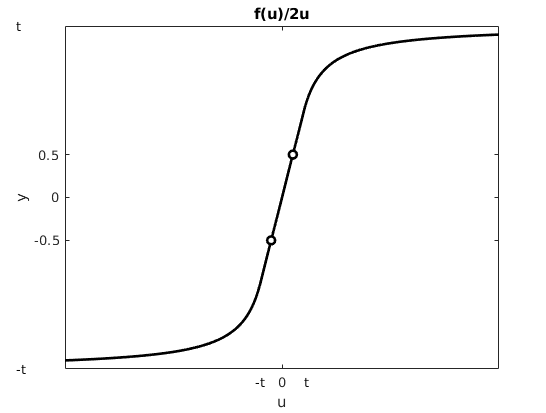
\includegraphics[width=0.5\textwidth]{./figs/nn/huber_sigmoid.png}
        \caption{Huber Sigmoid}
        \label{fig:huber_sigmoid}
    \end{figure}
    \begin{figure}[h!]
        \centering
        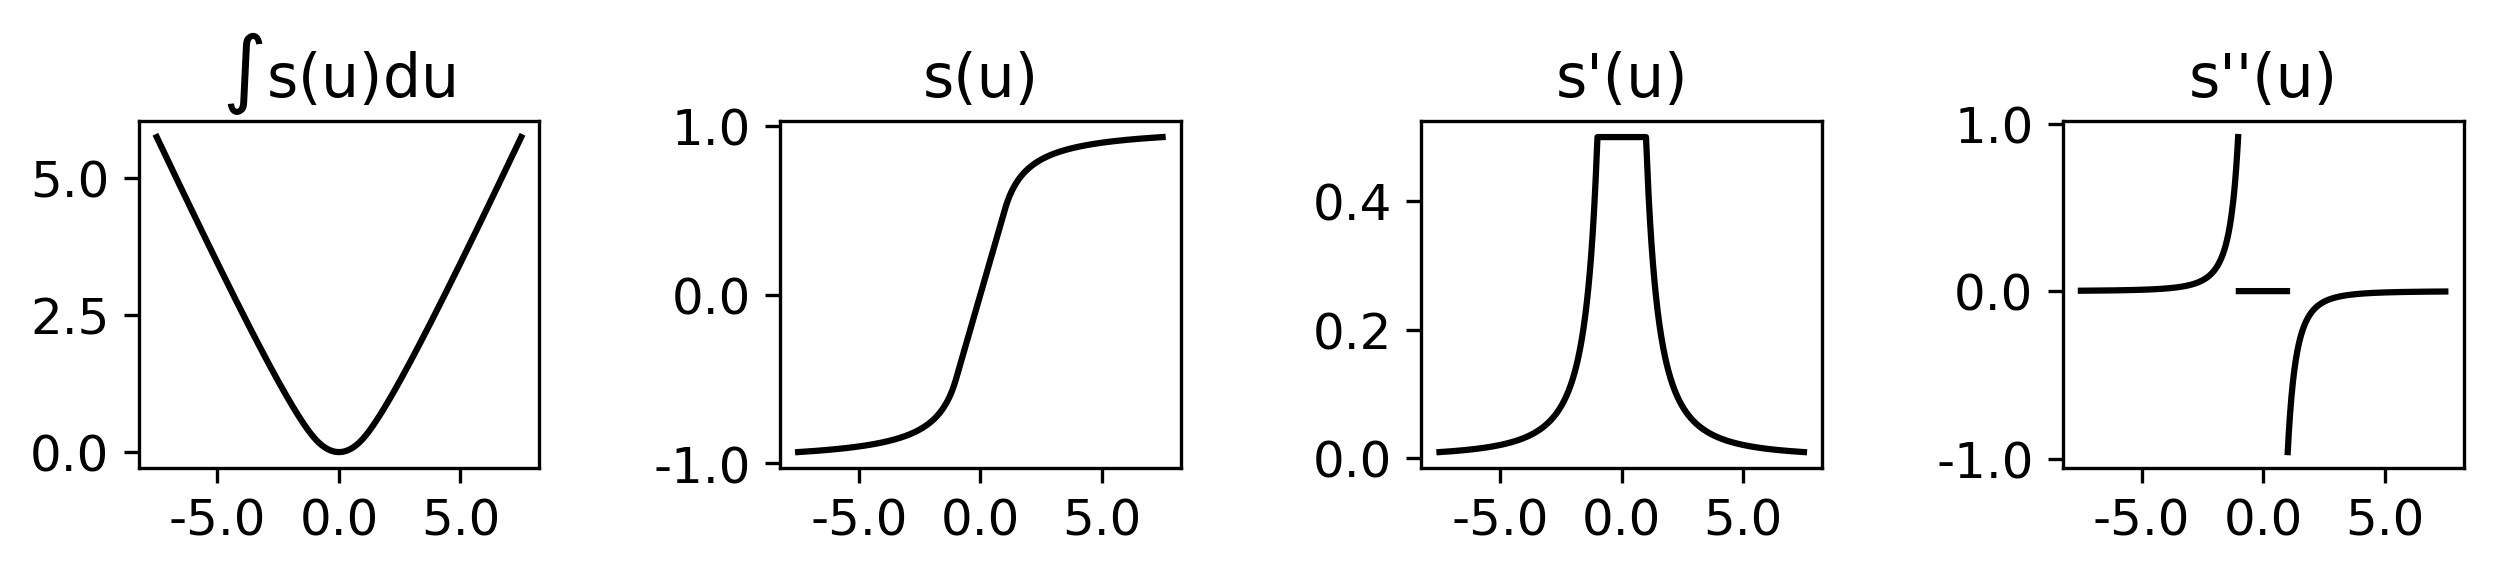
\includegraphics[width=0.7\textwidth]{./figs/nn/sig/Huber.png}
        \caption{Huber Sigmoid}
        \label{fig:sig_Huber}
    \end{figure}
    \clearpage

\subsection{Misc. Sigmoids}
\subsubsection{Trig Sigmoids}
    \begin{figure}[h!]
        \centering
        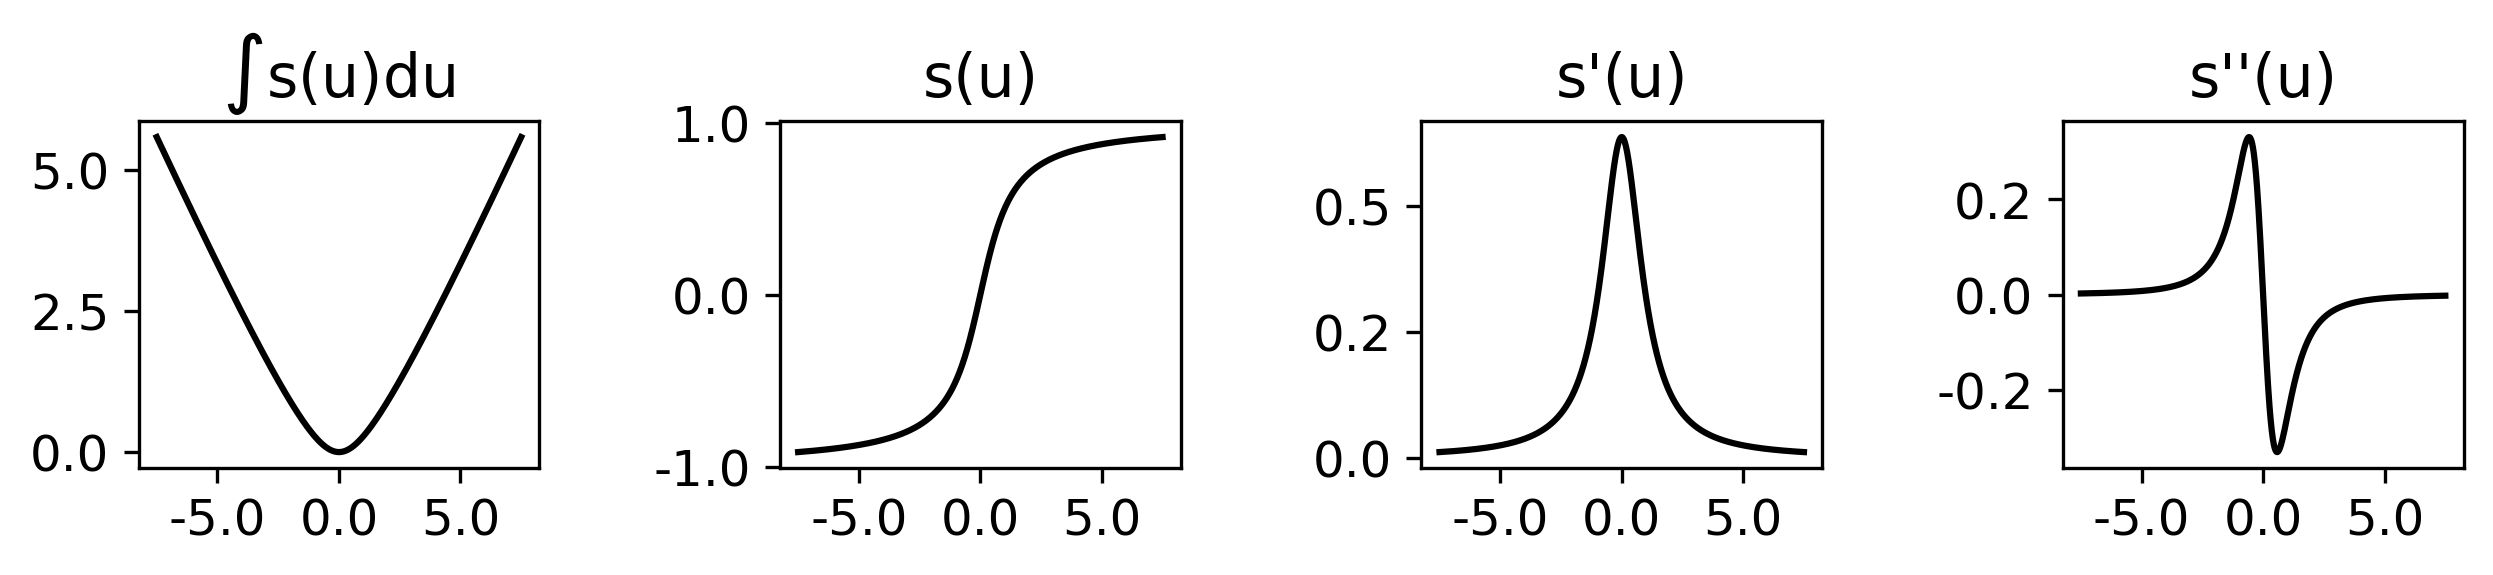
\includegraphics[width=0.7\textwidth]{./figs/nn/sig/atan.png}
        \caption{$\sig(u)=2\:\text{atan}(u)/\pi$}
        \label{fig:sig_atan}
    \end{figure}
    \begin{figure}[h!]
        \centering
        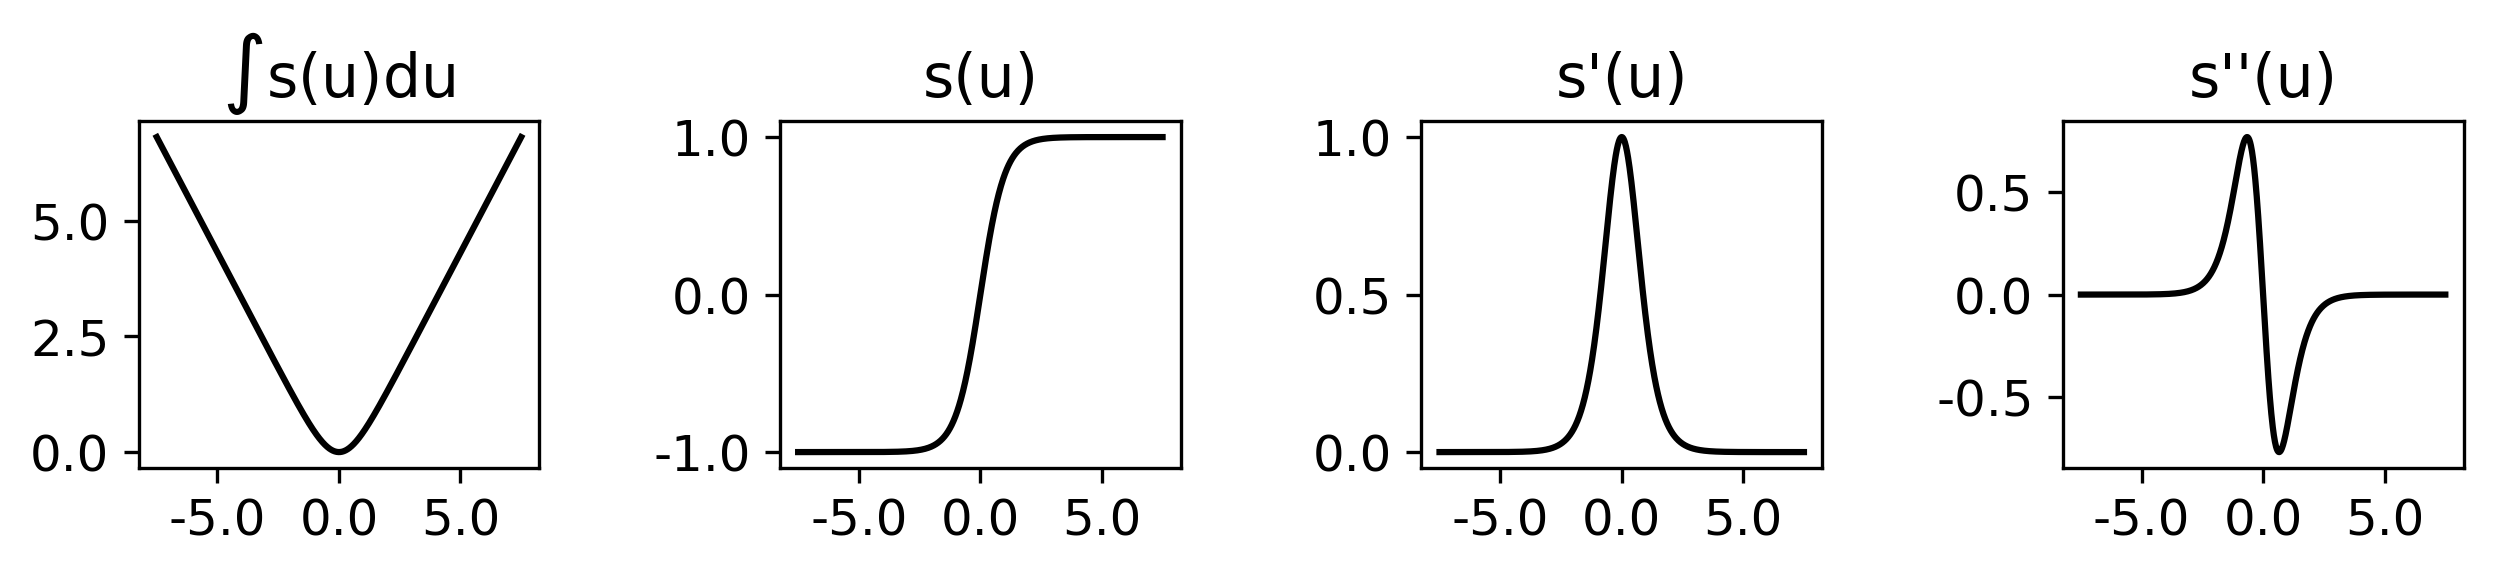
\includegraphics[width=0.7\textwidth]{./figs/nn/sig/tanh.png}
        \caption{$\sig(u)=\text{tanh}(u)$}
        \label{fig:sig_tanh}
    \end{figure}
    \begin{figure}[h!]
        \centering
        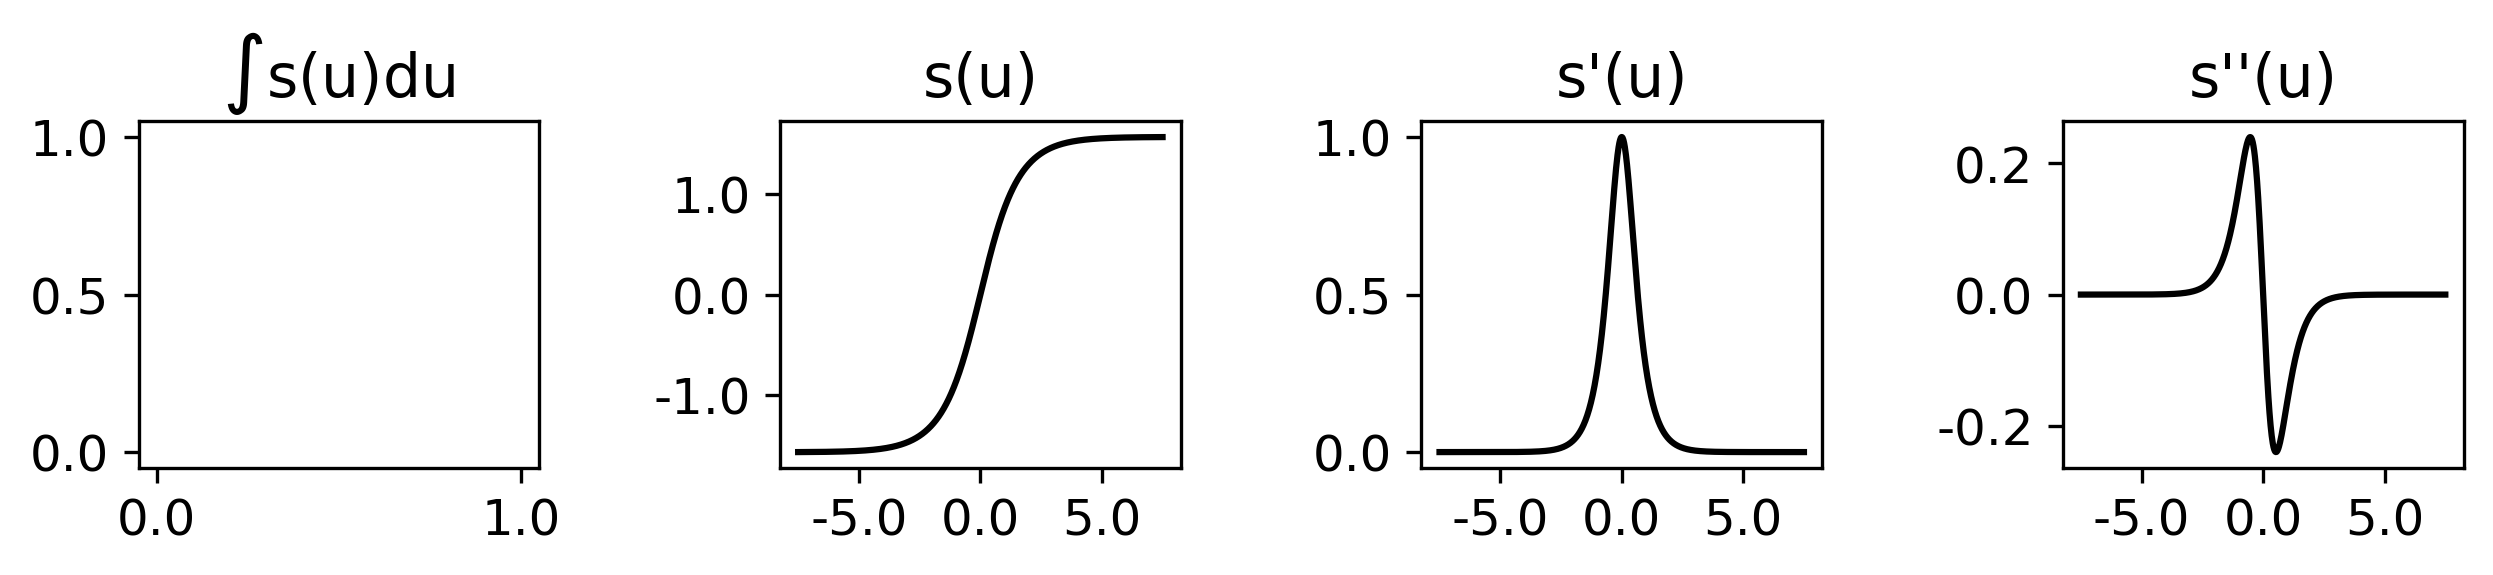
\includegraphics[width=0.7\textwidth]{./figs/nn/sig/gd.png}
        \caption{$\sig(u)=2\:\text{atan}\left(\text{tanh}(u/2)\right)$}
        \label{fig:sig_gd}
    \end{figure}
\subsubsection{Exponential Sigmoids}
    \begin{figure}[h!]
        \centering
        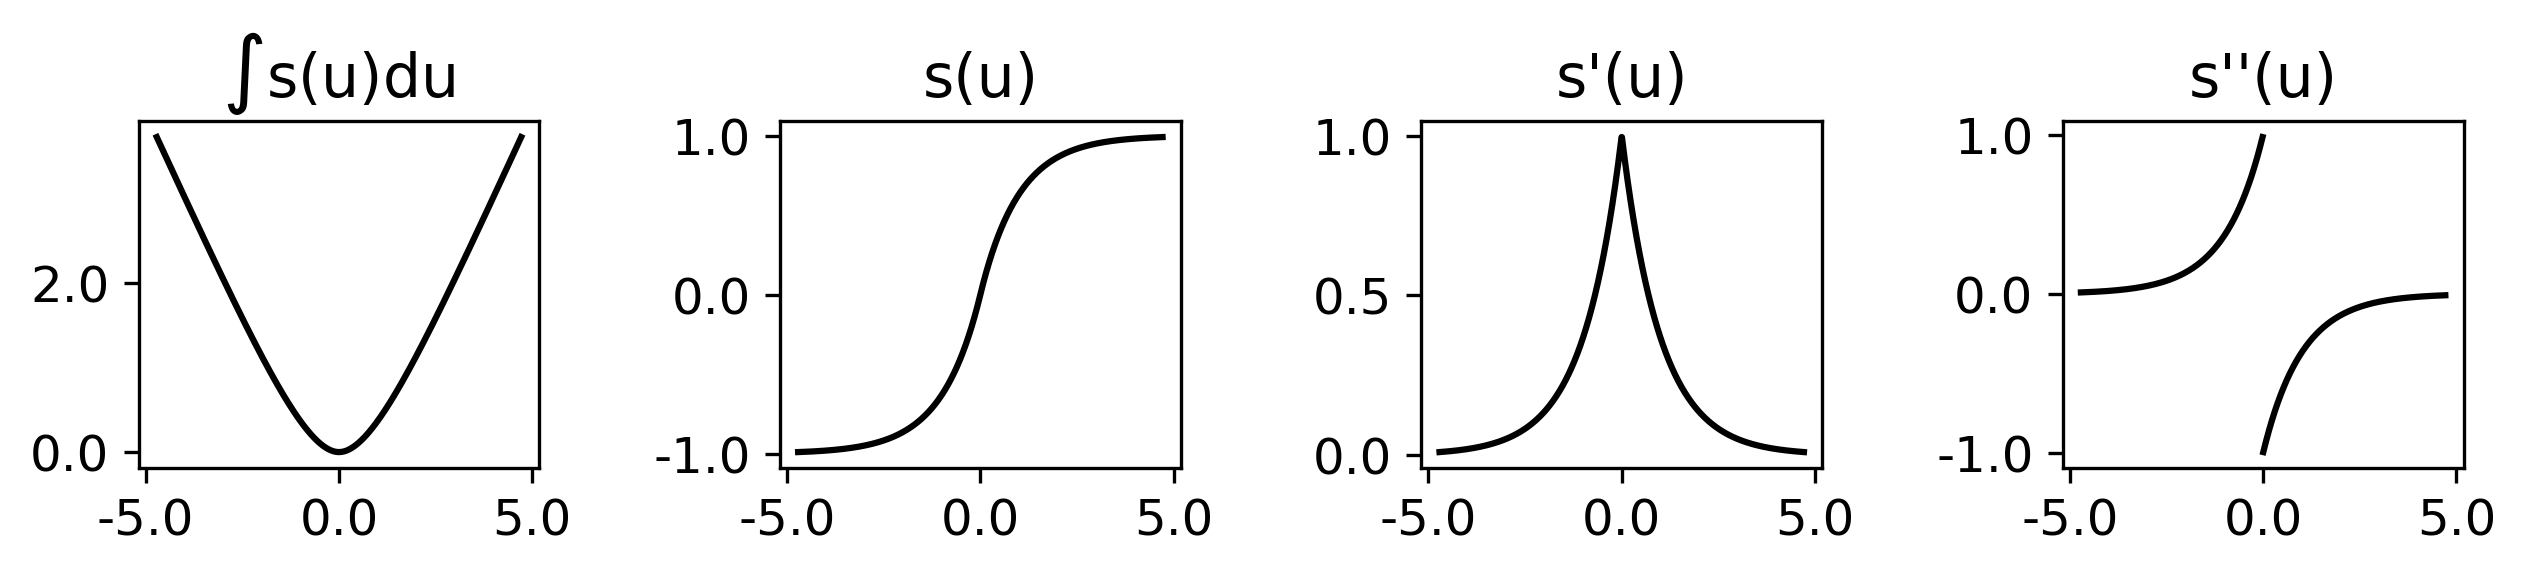
\includegraphics[width=0.7\textwidth]{./figs/nn/sig/exp.png}
        \caption{$\sig'(u)=\exp(-|u|)$}
        \label{fig:sig_exp}
    \end{figure} 
    \begin{figure}[h!]
        \centering
        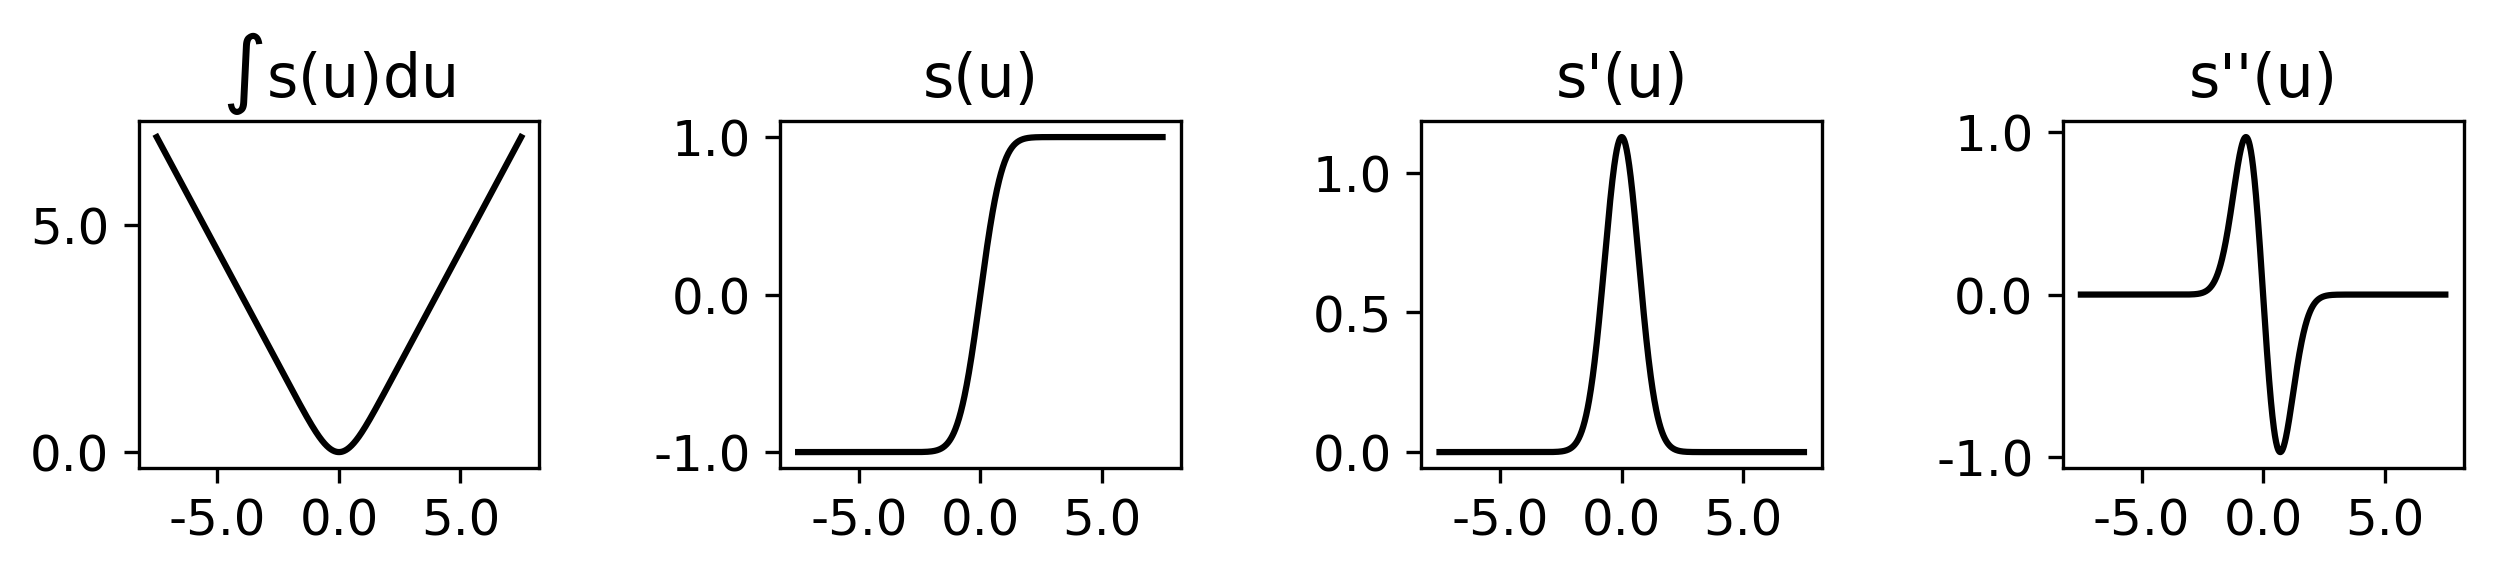
\includegraphics[width=0.7\textwidth]{./figs/nn/sig/Gauss.png}
        \caption{$\sig(u)=\text{erf}(u),\quad \sig'(u)=2\exp(-u^2)/\sqrt{\pi}$}
        \label{fig:sig_Gauss}
    \end{figure}

\clearpage

\subsubsection{Ramp Sigmoid}
    Ramp velocity profiles are common in robotics applications,
    e.g. Figure \ref{fig:sig_ramp}.
    \begin{figure}[h!]
        \centering
        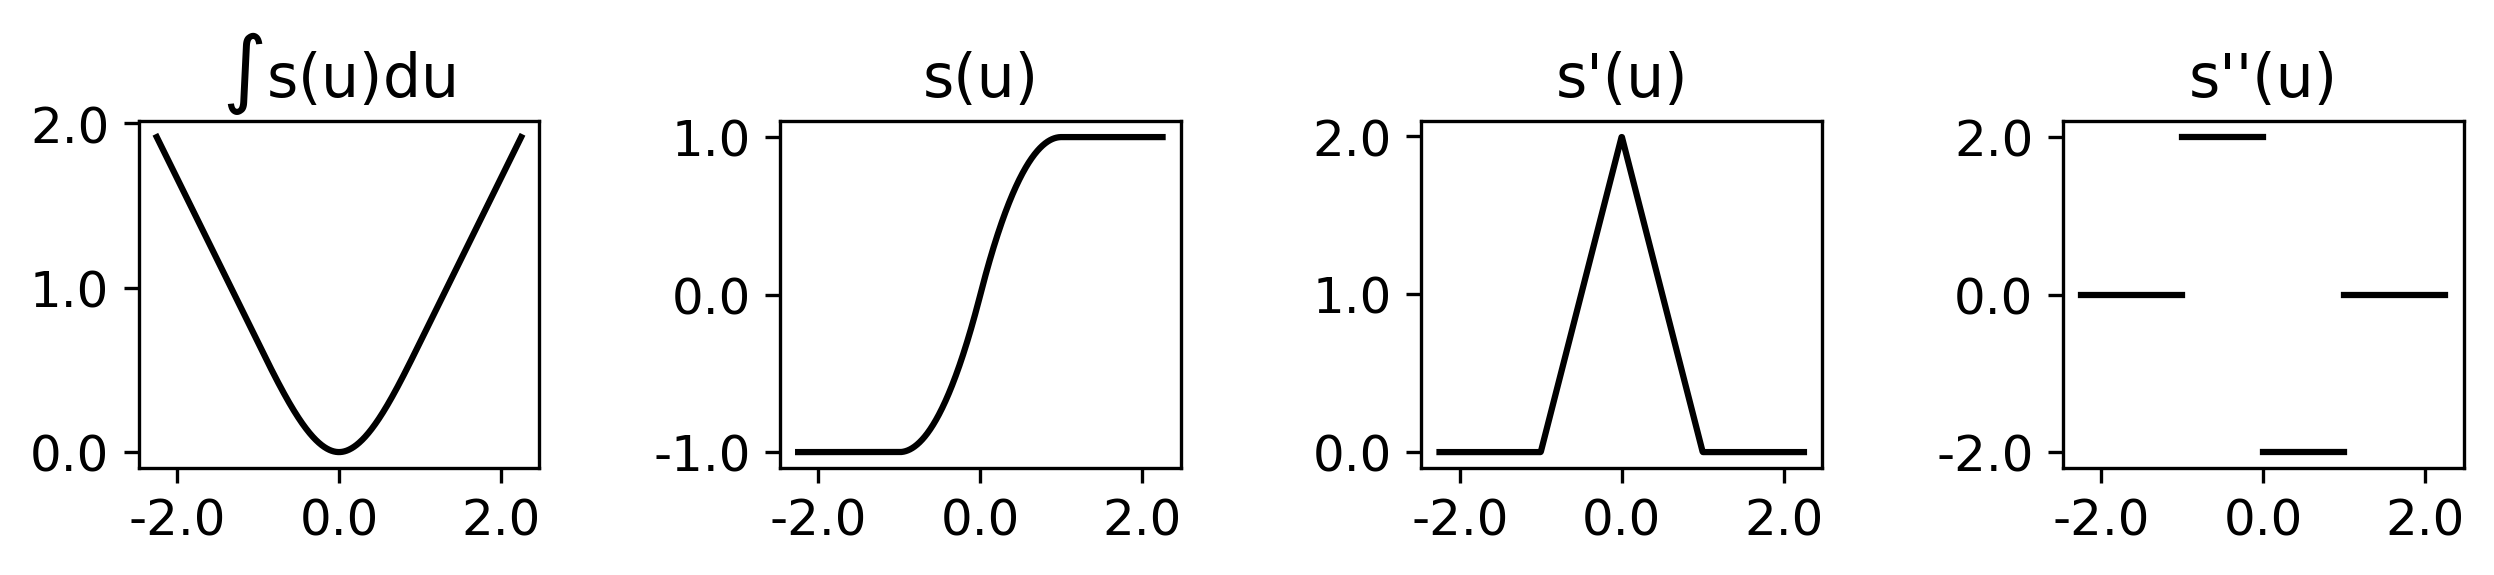
\includegraphics[width=0.7\textwidth]{./figs/nn/sig/trap.png}
        \caption{Ramp}
        \label{fig:sig_ramp}
    \end{figure} 

\subsubsection{Parabolic Sigmoids}
    \begin{figure}[h!]
        \centering
        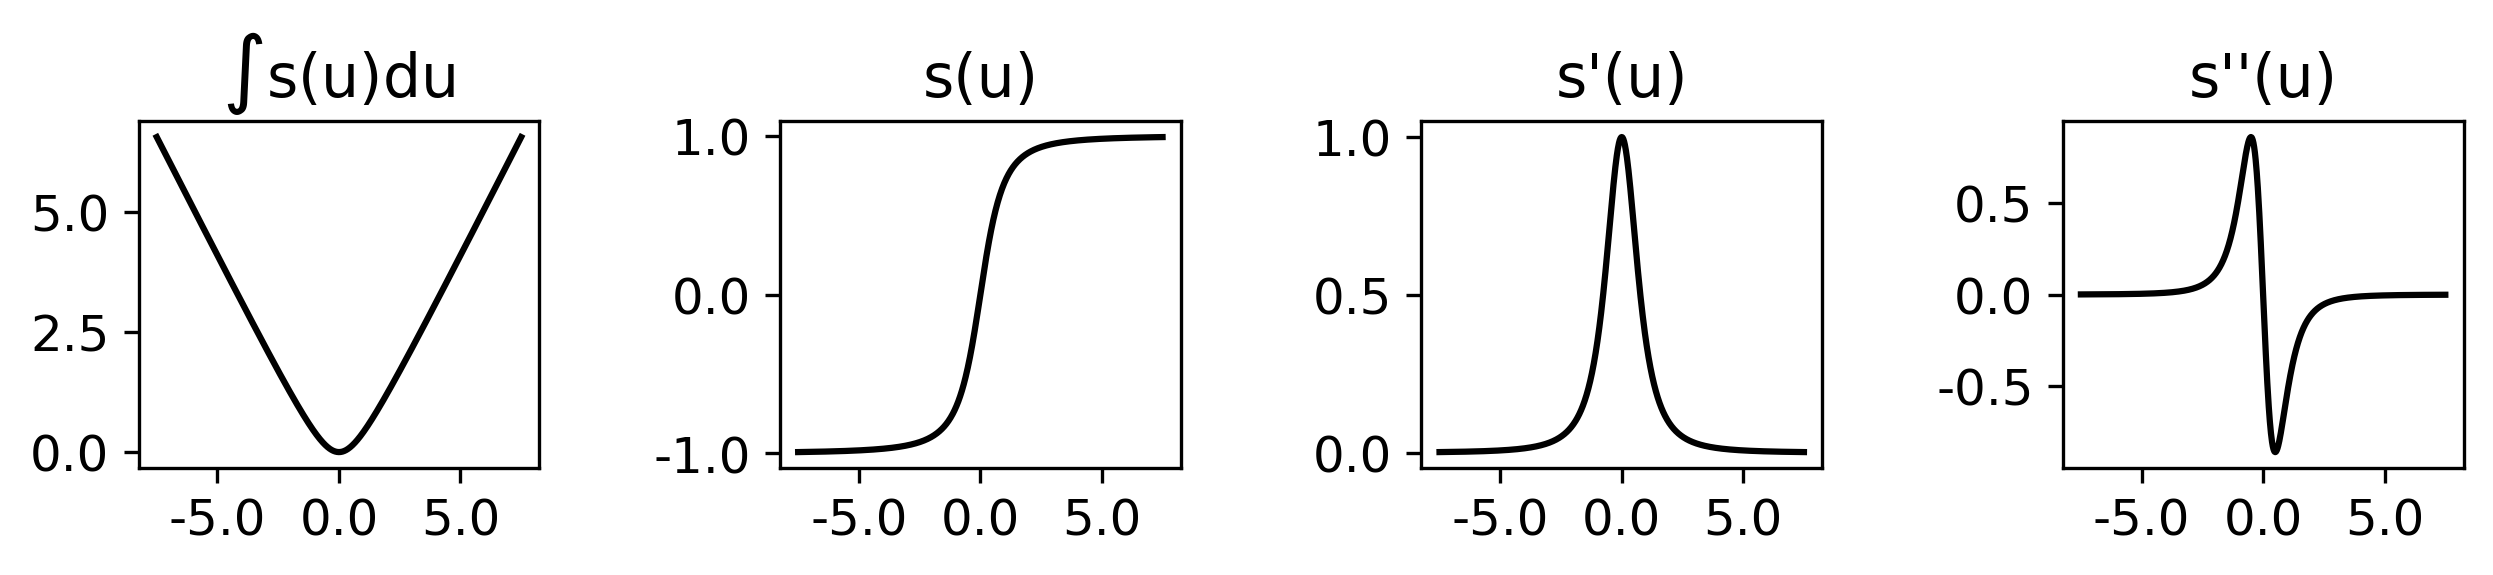
\includegraphics[width=0.7\textwidth]{./figs/nn/sig/parabola.png}
        \caption{$\sig(u)=u/\sqrt{1+u^2},\quad \int\sig(u)du = \sqrt{1+u^2}-1$}
        \label{fig:sig_parabola}
    \end{figure}

\subsubsection{Reciprocal Sigmoids}

    To obtain sigmoids with slow asymptotic convergence,
    consider reciprocal functions, e.g., linear--reciprocal (Figure \ref{fig:sig_inv_lin})
    \begin{align*}
        s(u)&=
        \left\{
        \arr{
                (1/u-1)^{-1} & \text{if}\quad u<0\\
        (1/u+1)^{-1} & \text{else}
        }    
        \right.,
    \end{align*}
    or log--reciprocal (Figure \ref{fig:sig_inv_log})
    \begin{align*}
        s(u)&=
        \left\{
        \arr{
                \minus\log(2)
                \log(2-u)^{-1}-1 & \text{if}\quad u<0\\
        -\log(2)\log(2+u)^{-1}+1 & \text{else}
        }    
        \right..
    \end{align*}
    These sigmoids both have an $s'(u)$ that converges to 0 very slowly.

    \begin{figure}[h!]
        \centering
        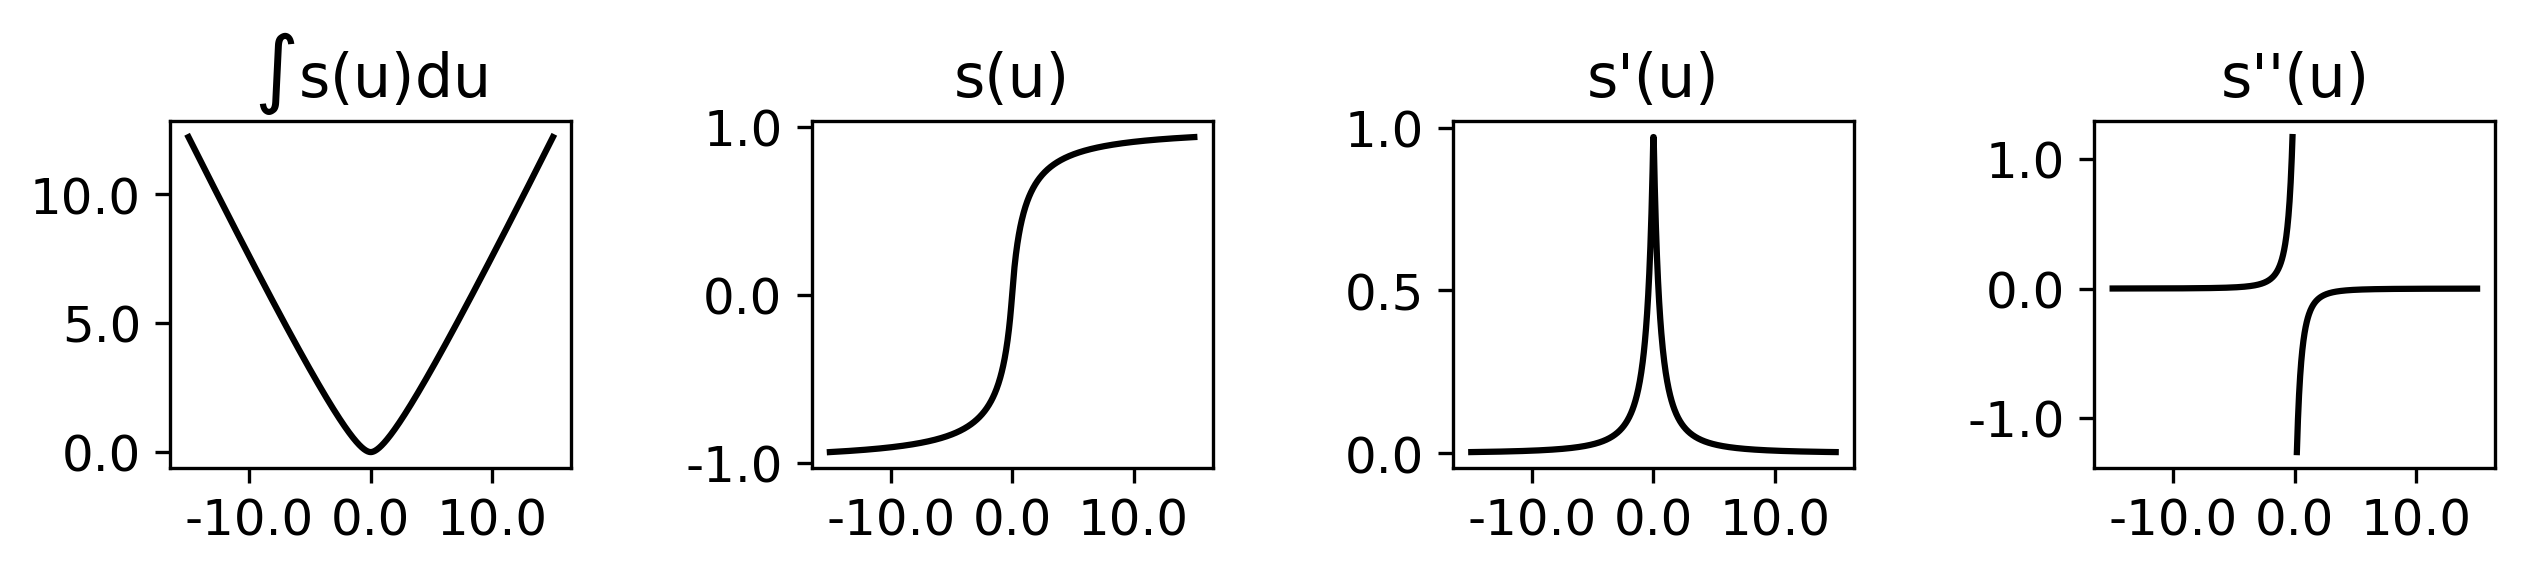
\includegraphics[width=0.7\textwidth]{./figs/nn/sig/inv_lin.png}
        \caption{Reciprocal Linear}
        \label{fig:sig_inv_lin}
    \end{figure}
    \begin{figure}[h!]
        \centering
        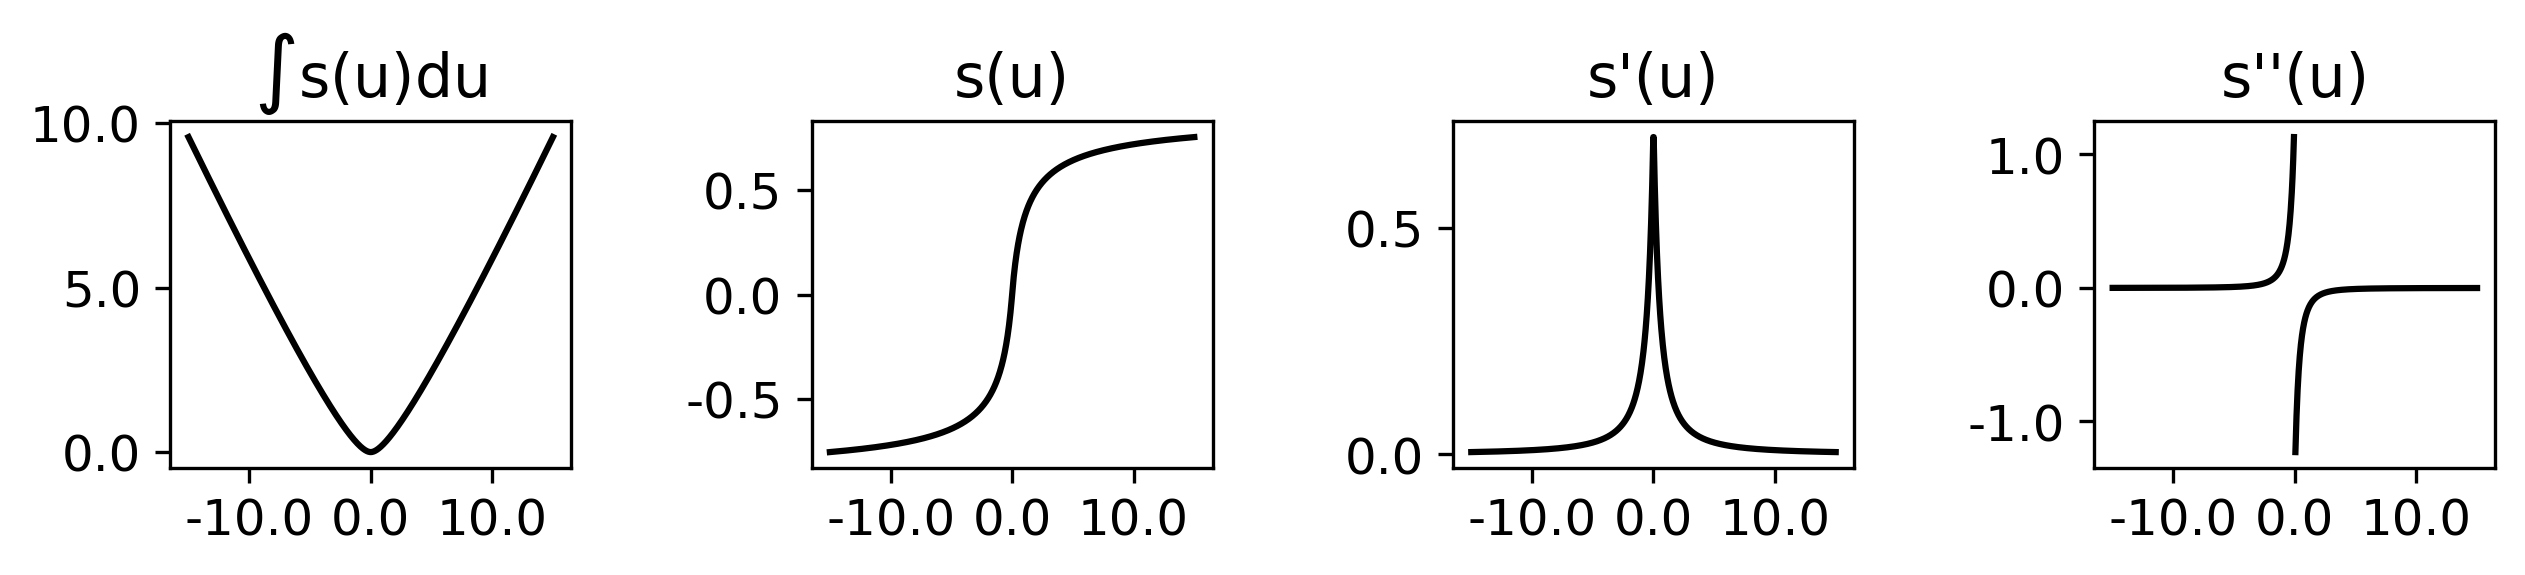
\includegraphics[width=0.7\textwidth]{./figs/nn/sig/inv_log.png}
        \caption{Reciprocal Log}
        \label{fig:sig_inv_log}
    \end{figure}

\clearpage

\section{NN: Neural Networks}\label{sec:nn} 

    Classical multi--layer perceptrons have been around for several decades.
    They are well--suited to learning mappings between Boolean tables
    but suffered early set backs (not living up to the early hype).
    In recent years,
    there has a been a resurgence in neural network research with fantastic results
    in classification \cite{yolo} and generation of complex data sets
    from easily interperted low level features
    \cite{img2img}, \cite{stylegan}.  
    The discoveries that have made this possible are pre-- and post--filters
    that provide appropriately conditioned output for classical 
    multi--layer perceptrons to excel, e.g., VAE (variational auto--encoders) and 
    CNN (convolutional neural networks).  
    These filters convert complex data into easily seperable or predictable features.
    In the case of CNN, these features are much larger than the input.
    In the case of VAE, these features are much smaller than the input.

    Using only multi--layer perceptrons injected with noise,
    generative methods (mapping low feature spaces to complex data spaces) have
    recently proven more powerful than state--of--the--art Markov--based methods.
    One of my rearch goals is to combine cascading RBST with
    the machinery of RNN, GAN, and LSTM to find scalable real--world application,
    similar to the results of \cite{world} but on a much larger scale.

    The forward calculation of an $n$-layer network mapping 
    $x$ to $y$ is shown in Algorithm \ref{algo:forward_NN}.
    Neural networks are nonlinear and non--convex, 
    but their optimization is greatly aided with a deeper understanding of \QP.
    Using the nonlinear \QP solvers in this repo, 
    many modifications to vanilla back--propogated $\ell_2$ error
    can be explored, e.g.,
    p--norm regularization,
    p--norm constraint,
    upper and lower parameter bounds, 
    relaxations with slack variables, and
    robust penalties like Huber and dedzone.  
    Enhanced solvers that take advantage of sparsity and parallelization
    are also of interest.

    \begin{algorithm}[H]
        \SetAlgoLined
        $z_0\leftarrow \sig \left(A_0x-b_0\right)$\\
        \For{$i\in\Z[1,n-1]$}
        {
            $z_i\leftarrow \sig \left(A_iz_{i-1}-b_i\right)$
        }
        \Return $y\leftarrow z_{n-1}$
    \caption{Forward NN}
    \label{algo:forward_NN} 
    \end{algorithm}

\subsection{1--Layer Perceptron} 

    For $h:\R^n\to\R^m$, let
    \begin{align*}
        \sig(h)&=\row\{\sig(h_i)\}_{i=0}^{m-1},\\
        \sig'(h)&=\diag\{\sig'(h_i)\}_{i=0}^{m-1},
    \end{align*}
    where $\sig$ could be any of the proposed functions in the sigmoid section.\\
    For $x\in\R^n$ and $y\in\R^m$, consider
    \begin{align*}
        \min_{\{A,b\}\in\{\R^{m\times n},\R^m\}}\quad 
        \sum_{\{x,y\}} J (x,y),
    \end{align*}
    where
    \begin{align*}
        J(x,y)&=\frac{1}{2}\|\sig(Ax -b)-y \|_{2,W(x,y)}^2\\
        &=\frac{1}{2}\|z-y \|_{2,W(x,y)}^2,            
    \end{align*}
    and
    \begin{align*}
        z&=\sig(Ax-b)\\
        &=\sig((\eye_m\otimes x ^\tp)\vec{A}-b).
    \end{align*}
    Let
    \begin{align*}
        w=W^\tp W(z-y ).
    \end{align*}
    The partials are
    \begin{align*}
        \pd{ J }{x}&=w^\tp \pd{z}{x},\\\\
        \pd{ J }{\vec{A}}&=w^\tp  \pd{z}{\vec{A}},\\\\
        \pd{ J }{b}&=w^\tp \pd{z}{b},
    \end{align*}
    where
    \begin{align*}
        \pd{z}{x}&=\sig'(Ax-b)A,\\\\
        \pd{z}{\vec{A}}&=\sig'(Ax-b)(\eye_m\otimes x ^\tp),\\\\
        \pd{z}{b}&=-\sig'(Ax-b).
    \end{align*}

\subsection{2--Layer Perceptron}

    For $z_i\in\R^{m_i}$ with $i\in\Z[0,n-1]$ and $n=2$, consider
    \begin{align*}
        \min_{\{A_i,b_i\}\in\{\R^{m_i\times m_{i-1}},\R^{m_i}\}}\quad 
        \sum_{\{x,y\}}
        J (x,y),
    \end{align*}
    where
    \begin{align*}
        J(x,y)&=\frac{1}{2}\|\sig(A_1\sig(A_0x -b_0)-b_1)-y \|_{2,W(x,y)}^2\\
        &=\frac{1}{2}\|z_1-y \|_{2,W(x,y)}^2,        
    \end{align*}
    and
    \begin{align*}
        z_0&=\sig(A_0x -b_0),\\
        z_1&=\sig(A_1z_0-b_1).
    \end{align*}
    Let
    \begin{align*}
        w=W^\tp W (z_1-y ).
    \end{align*}
    The partials for $A_i$ and $b_i$ are
    \begin{align*}
        \pd{ J }{\vec{A}_1}&=w^\tp  \pd{z_1}{\vec{A}_1},\\
        \pd{ J }{\vec{A}_0}&=w^\tp  \pd{z_1}{z_0}\pd{z_0 }{\vec{A}_0},\\
        \\
        \pd{ J }{b_1}&=w^\tp  \pd{z_1}{b_1},\\
        \pd{ J }{b_0}&=w^\tp  \pd{z_1}{z_0}\pd{z_0 }{b_0},
    \end{align*}
    where
    \begin{align*}
        \pd{z_1}{z_0}&=\sig'(A_1z_0 -b_1)A_1,\\\\
        \pd{z_1}{\vec{A}_1}&=\sig'(A_1z_0 -b_1)(\eye_{m_1}\otimes z_0 ^\tp),\\
        \pd{z_1}{b_1}&=-\sig'(A_1z_0 -b_1),\\\\
        \pd{z_0}{\vec{A}_0}&=\sig'(A_0x -b_0)( \eye_{m_0} \otimes x ^\tp)\\
        \pd{z_0}{b_0}&=-\sig'(A_0x -b_0).
    \end{align*}
    
\subsection{3--Layer Perceptron}\label{sec:nn3}

    For $z_i\in\R^{m_i}$ with $i\in\Z[0,n-1]$ and $n=3$, consider
    \begin{align*}
        \min_{\{A_i,b_i\}\in\{\R^{m_i\times n_i},\R^{m_i}\}}\sum_{\{x,y\}}
        J (x,y)
    \end{align*}
    where
    \begin{align*}
        J(x,y)&=\frac{1}{2}\|\sig(A_2\sig(A_1\sig(A_0x-b_0)-b_1)-b_2)-y \|_{2,W(x,y)}^2\\
        &=\frac{1}{2}\|z_2-y \|_{2,W(x,y)}^2,
    \end{align*}
    and
    \begin{align*}
        z_0&=\sig(A_0x-b_0),\\
        z_1&=\sig(A_1z_0-b_1),\\
        z_2&=\sig(A_2z_1-b_2).
    \end{align*}
    Let
    \begin{align*}
        w=W^\tp W(z_2-y ).
    \end{align*}
    The partials for $A_i$ and $b_i$ are
    \begin{align*}
        \pd{ J }{\vec{A}_2}&=w^\tp  \sig'(A_2z_1 -b_2)(\eye_{m_2}\otimes z_1^\tp),\\
        \pd{ J }{\vec{A}_1}&=w^\tp  \sig'(A_2z_1 -b_2)A_2\sig'(A_1z_0 -b_1)(\eye_{m_1}\otimes z_0^\tp),\\
        \pd{ J }{\vec{A}_0}&=w^\tp  \sig'(A_2z_1 -b_2)A_2\sig'(A_1z_0 -b_1)A_1\sig'(A_0x -b_0)( \eye_{m_0} \otimes x ^\tp),\\
        \\
        \pd{ J }{b_2}&=-w^\tp  \sig'(A_2z_1 -b_2),\\
        \pd{ J }{b_1}&=-w^\tp  \sig'(A_2z_1 -b_2)A_2\sig'(A_1z_0 -b_1),\\
        \pd{ J }{b_0}&=-w^\tp  \sig'(A_2z_1 -b_2)A_2\sig'(A_1z_0 -b_1)A_1\sig'(A_0x -b_0).
    \end{align*}
    
    \clearpage
\subsection{n--Layer Perceptron}

    In general, for $z_i\in\R^{m_i}$ with $i\in\Z[0,n-1]$, consider
    \begin{align*}
        \min_{\{A_i,b_i\}\in\{\R^{m_i\times m_{i-1}},\R^{m_i}\}}\quad 
        \sum_{\{x,y\}}&=J(x,y),
    \end{align*}
    where
    \begin{align*}
        J(x,y)=\frac{1}{2}\|z_{n-1}-y \|_{2,W(x,y)}^2.
    \end{align*}
    For $i\in\Z[1,n-1]$,
    \begin{align*}
        z_i&=\sig(A_iz_{i-1}-b_i),
    \end{align*}
    with
    \begin{align*}
        z_0&=\sig(A_0x-b_0).
    \end{align*}
    Let
    \begin{align*}
        w=  W^\tp W (z_{n-1}-y).
    \end{align*}
    The partials are given by
    \begin{align*}
        \pd{ J }{\vec{A}_i}&=w^\tp \pd{z_{n-1}}{z_{n-2}}\pd{z_{n-2}}{z_{n-3}}\cdots
        \pd{z_{i+1}}{z_i}\pd{z_i}{\vec{A}_i},\\
        \pd{ J }{b_i}&=w^\tp \pd{z_{n-1}}{z_{n-2}}\pd{z_{n-2}}{z_{n-3}}\cdots
        \pd{z_{i+1}}{z_i}\pd{z_i}{b_i},
    \end{align*}
    where
    \begin{align*}
        \pd{z_j}{z_{j-1}}&=\sig'(A_jz_{j-1} -b_j)A_j,\\
        \pd{z_j}{\vec{A}_j}&=\sig'(A_jz_{j-1} -b_j)(\eye_{m_j}\otimes z_{j-1} ^\tp),\\
        \pd{z_j}{b_j}&=-\sig'(A_jz_{j-1} -b_j).
    \end{align*}

\subsection{n--Layer Perceptron with States}

    For $z_i\in\R^{m_i}$ with $i\in\Z[0,n-1]$ , consider
    \begin{align*}
        \min_{\{z_i(x),A_i,b_i\}\in\{\R^{m_i},\R^{m_i\times m_{i-1}},\R^{m_i}\}}
        \quad \sum_{\{x,y\}}
        J (x,y)&=\frac{1}{2}\|z_{n-1}-y \|_{2,W(x,y)}^2,
    \end{align*}
    with
    \begin{align*}
        f_\eq(z,A,b|x)=\mat{
        z_0-\sig(A_0x-b_0)\\
        z_1-\sig(A_1z_0-b_1)\\
        \vdots&\\
        z_{n-1}-\sig(A_{n-1}z_{n-2}-b_{n-1})}=\zeros^M,
    \end{align*}
    where
    \begin{align*}
        r=\sum_{i=0}^{n-1}m_i.
    \end{align*}

    This formulation resembles MPC.  
    The nonlinear equality constraint can be implamented 
    with any of the methods presented in seciton \ref{sec:np_constraint}.
    Adding states adds a degree of freedom in the optimization 
    that might help in cases where the gradient would traditionally vanish.
    The disadvantage to this approach is, 
    for $q$ sample pair of $\{x,y\}$, there are $rq$ new free variables to optimize.

    \clearpage
\subsection{ML: Maximum Likelihood}

    Consider the probability model
    \begin{align*}
        p=\nn(x),
    \end{align*}
    with 
    \begin{align*}
        p&=\prob(\rand{y}=1),\\
        1-p&=\prob(\rand{y}=0).
    \end{align*}
    
    Collect $x\in\{0,1\}^n$ and sort them by $y=1$ and $y=0$.

    ML formulates the problem
    \begin{align*}
        \min_{\{A_i,b_i\}\in\{\R^{m_i\times m_{i-1}},\R^{m_i}\}}\quad J &= -l\\
        &=-\log\left(\prod_{x\:\text{with}\:y=1}p(x)
            \prod_{x\:\text{with}\:y=0}(1-p(x))\right)\\\\
        &=-\sum_{x\:\text{with}\:y=1}\log \left(\nn(x)\right)
        -\sum_{x\:\text{with}\:y=0} \log\left(1-\nn(x)\right).
    \end{align*}

    With $\nn(x)=z_{n-1}(x)$ and $z_{n-1}\in\R[0,1]$, the partials are given by

    \begin{align*}
        \pd{ J }{\vec{A}_i}&=\left\{
            \arr{
                -\dfrac{1}{z_{n-1}} \pdLARGE{z_{n-1}}{z_{n-2}}\pdLARGE{z_{n-2}}{z_{n-3}}\cdots
        \pdLARGE{z_{i+1}}{z_i}\pdLARGE{z_i}{\vec{A}_i}
        & \text{if}\quad y=1\\\\
        \dfrac{1}{1-z_{n-1}} \pdLARGE{z_{n-1}}{z_{n-2}}\pdLARGE{z_{n-2}}{z_{n-3}}\cdots
        \pdLARGE{z_{i+1}}{z_i}\pdLARGE{z_i}{\vec{A}_i}
        & \text{if}\quad y=0
        }\right.,\\\\\\
        \pd{ J }{b_i}&=\left\{
            \arr{
                -\dfrac{1}{z_{n-1}} \pdLARGE{z_{n-1}}{z_{n-2}}\pdLARGE{z_{n-2}}{z_{n-3}}\cdots
                \pdLARGE{z_{i+1}}{z_i}\pdLARGE{z_i}{b_i}
        & \text{if}\quad y=1\\\\
        \dfrac{1}{1-z_{n-1}} \pdLARGE{z_{n-1}}{z_{n-2}}\pdLARGE{z_{n-2}}{z_{n-3}}\cdots
        \pdLARGE{z_{i+1}}{z_i}\pdLARGE{z_i}{b_i}
        & \text{if}\quad y=0
        }\right.,
    \end{align*}
    where
    \begin{align*}
        \pd{z_j}{z_{j-1}}&=\sig'(A_jz_{j-1} -b_j)A_j,\\\\
        \pd{z_j}{\vec{A}_j}&=\sig'(A_jz_{j-1} -b_j)(\eye_{m_j}\otimes z_{j-1} ^\tp),\\\\
        \pd{z_j}{b_j}&=-\sig'(A_jz_{j-1} -b_j),
    \end{align*}
    and
    \begin{align*}
        s(u)=(1+e^{-u})^{-1}.
    \end{align*}

\clearpage

\section{MPC: Model Predictive Control}

    Let
    \begin{align*}
        u_t&=\text{input},\\
        y_t&=\text{output},\\
        z_t&=\text{hidden internal dynamic state},\\
        \theta_{\phantom{t}}&=\text{hidden internal constant state}.
    \end{align*}
    MPC uses models of the form 
    \begin{align*}
        z_{t+1}&=f(z_t,u_t|\theta)\\
        y_t &= g(z_t,u_t|\theta)
    \end{align*}
    The models may be nonlinear or generalized deep neural networks, but if they can
    be expressed as linear, then \QP can be used to solve them in one iteration.
    Time will be analyzed on a sliding window where $t=0$ depicts the present 
    (Figure \ref{fig:world_model_time}).
    The world takes input and produces output over this moving time window
    (Figure \ref{fig:world_model_world}).
    It is assumed that the world has some hidden internel dynamic states
    that need to be determined.  
    The quantitative expression of these states depends on the model
    chosen to approximate the world.  An estimator uses the model and the observed
    input and output history to produce a best current guess of the dynamic and constant
    hidden states (Figure \ref{fig:world_model_estimator}).
    Once the current best guess is given for the states,
    the controller uses the model along with target
    input and output to find the optimal future input
    (Figure \ref{fig:world_model_controller}).
    These calculations are done each time step on hardware, 
    \begin{itemize}
        \item estimating $z_0^*$ and $\theta^*$ from $u[-T,0)$ and $y[-T,0]$,
        \item and computing and applying $u_0^*$ from $z_0^*$ and $\theta^*$.
    \end{itemize}

    Lectures on MPC can be found here \cite{mpc} and here \cite{bv_mpc}. 
    There are many interesting applications in walking and flying robotics,
    including \cite{mit}, \cite{eth}, and \cite{dandrea}.  
    Additional examples can be found at \cite{tedrake} and \cite{abbeel}.
    Python packages can be found here \cite{osqp}.
    Pytorch extensions can be found here \cite{mpc_pytorch}.

    \begin{figure}[h!]
        \centering
        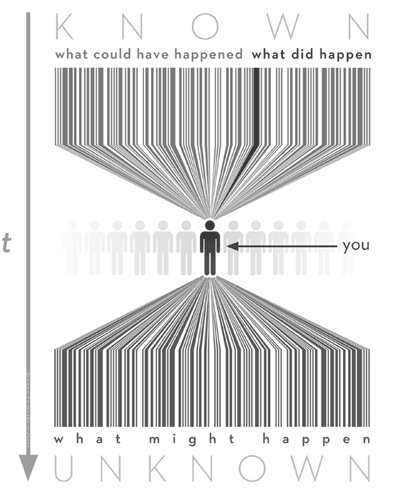
\includegraphics[width=.5\textwidth]{./figs/mpc/mpc.png}
        \caption{MPC}
        \label{fig:mpc_futurism}
    \end{figure}

    \clearpage
    \begin{figure}[h!]
        \centering
        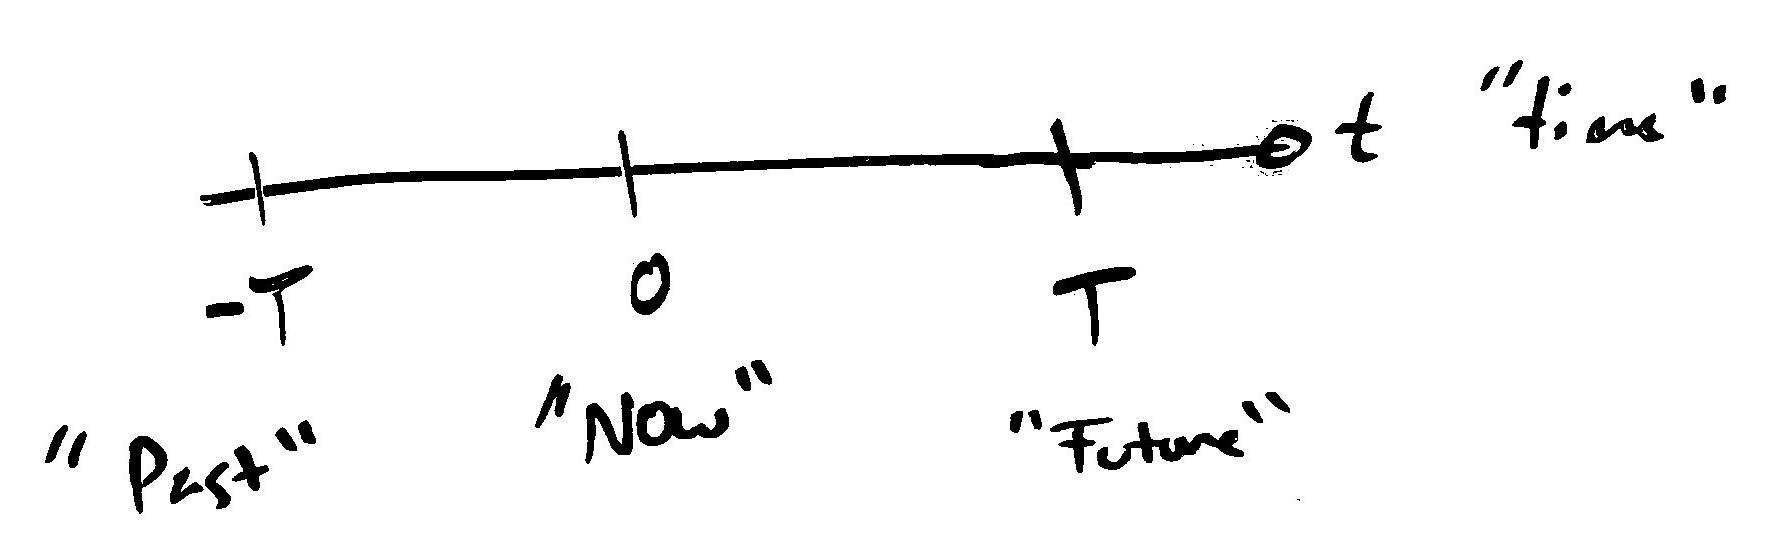
\includegraphics[width=0.5\textwidth]{./figs/mpc/world_model_time.jpg}
        \caption{Time}
        \label{fig:world_model_time}
    \end{figure}
    \begin{figure}[h!]
        \centering
        
\includegraphics[width=0.5\textwidth]{./figs/mpc/world_model_world.jpg}
        \caption{World}
        \label{fig:world_model_world}
    \end{figure}
    \begin{figure}[h!]
        \centering
        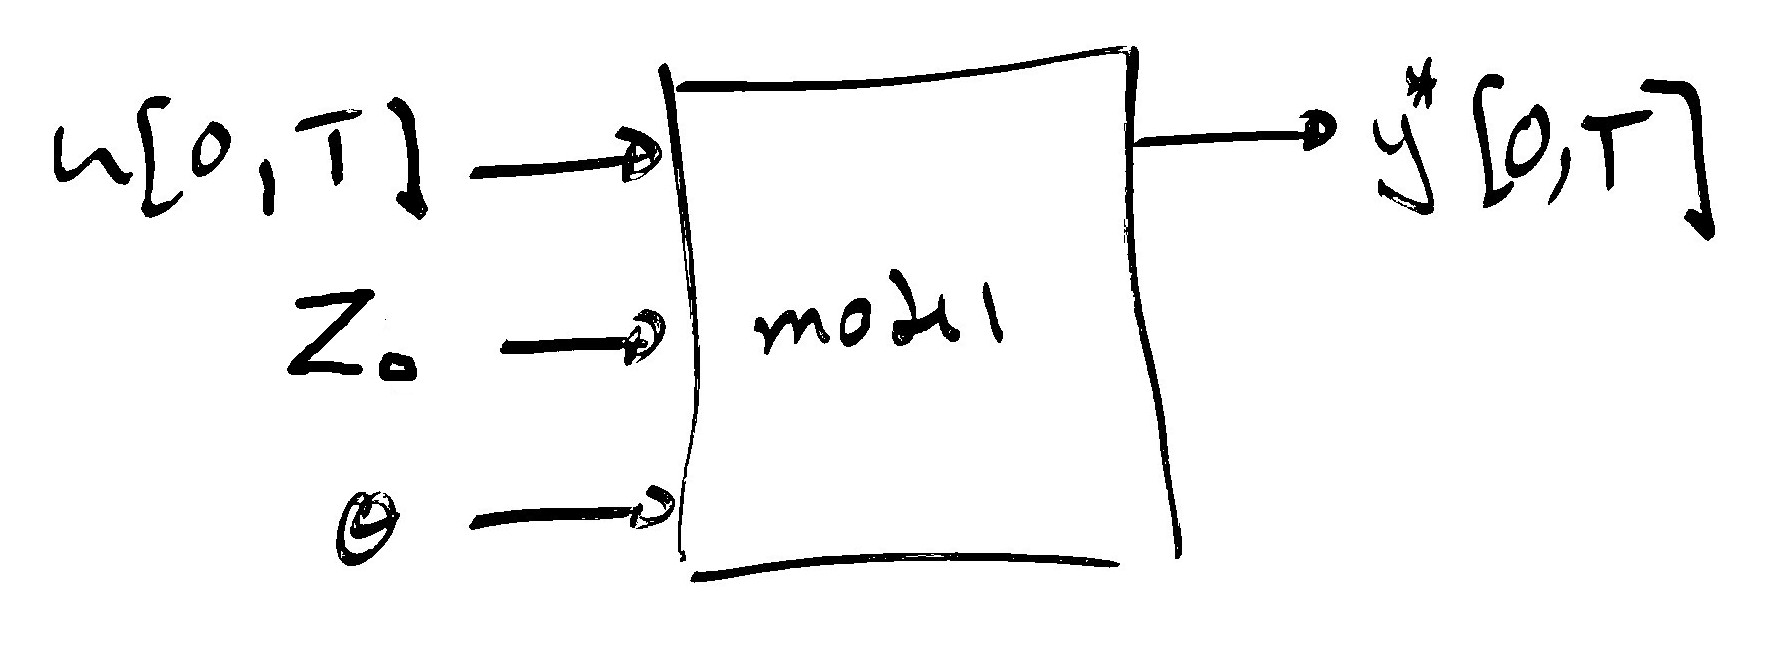
\includegraphics[width=0.5\textwidth]{./figs/mpc/world_model_model.jpg}
        \caption{World Model}
        \label{fig:world_model_model}
    \end{figure}
    \begin{figure}[h!]
        \centering
        \includegraphics[width=0.5\textwidth]{./figs/mpc/world_model_estimator.jpg}
        \caption{World Model Estimator}
        \label{fig:world_model_estimator}
    \end{figure}
    \begin{figure}[h!]
        \centering
        \includegraphics[width=0.5\textwidth]{./figs/mpc/world_model_controller.jpg}
        \caption{World Model Controller}
        \label{fig:world_model_controller}
    \end{figure}

    \clearpage

\subsection{LTV: Linear Time Variant}
    
    For $i\in\Z[0,q-1]$, consider the discrete-time system

    \begin{align*}
    z_{i+1} &= A_iz_i + B_iu_i,\\
    z_0 &= \text{fixed},
    \end{align*}

    where $u_i\in\R^m$ and $z_i\in\R^n$.
    For any selected time horizon $q$, 
    this system can be expressed as 

    \begin{align*}
        A_\eq x = b_\eq,
    \end{align*}

    where
    \begin{align*}
    x_i =
        \left[\begin{array}{l}
            u_i
            \\
            z_{i+1}
        \end{array}\right].
    \end{align*}
    For $q=3$,
    \begin{align*}
        \zeros^{n} &= A_0 z_0 + B_0 u_0 - z_1,   \\
        \zeros^{n} &= A_1 z_1 + B_1 u_1 - z_2,   \\
        \zeros^{n} &= A_2 z_2 + B_2 u_2 - z_3,
    \end{align*}
    which gives
    \begin{align*}
        \left[\begin{array}{ll|ll|ll}
                    B_0
                &
                    -\eye_n
                &
                    \zeros 
                &
                    \minus \zeros
                &
                    \zeros
                &
                    \minus \zeros
            \\
                    \zeros
                &
                    \minus A_1
                &
                    B_1                   
                &
                    -\eye_n
                &
                    \zeros
                &
                    \minus \zeros
            \\
                    \zeros
                &
                    \minus \zeros
                &
                    \zeros  
                &
                    \minus A_2
                &
                    B_2
                &
                    -\eye_n
        \end{array}
            \right]
        \mat{
            u_0\\
            z_1\\\hline
            u_1\\
            z_2\\\hline
            u_2\\
            z_3
            }&=\mat{
                -A_0z_0\\
                \minus \zeros\\
                \minus \zeros
            }.
    \end{align*}
    For $q>0$,
    \begin{align*}
        A_\eq&=\mat{\zeros^{n\times (m+n)(q-1)} & \zeros^{n\times (m+n)} \\
        \diag\{\mat{\zeros^{n\times m}&A_i}\}_{i=1}^{q-1} & \zeros^{n(q-1)\times(m+n)} }+
        \diag\{\mat{B_i&-\eye_n}\}_{i=0}^{q-1},\\
        b_\eq&=\mat{-A_0z_0\\
        \minus\zeros^{n(q-1)}}.
    \end{align*}

    \subsubsection{Block Components}

    The $u$ and $z$ components can be accessed with
    \begin{align*}
        u_{0:q-1}&=Gx,\\
        z_{1:q}&=Fx,
    \end{align*}
    where
    \begin{align*}
        G&=\diag\left\{\mat{\eye_m & \zeros^{m\times n}}\right\}_{i=0}^{q-1},\\
        F&=\diag\left\{\mat{\zeros^{n\times m}&\eye_n}\right\}_{i=0}^{q-1}.
    \end{align*}

    \subsubsection{Rate Regularization} 

    For weight $W_i\in\R^{m\times m}$, the input rate can be regularized by
    \begin{align*}
    \sum_{i=0}^{q-2}\left\|u_{i+1}-u_i\right\|_{W_i}
        &=\|u_{1:q-1}-u_{0:q-2}\|_{W}\\
            &=\|u_{0:q-1} \|_{WD},
    \end{align*}
    where \cite[p.~312]{bv_cvxbook}
    \begin{align*}
        D= \diag(\:\zeros^{m\times m},\:\eye_{m(q-1)}\:)-\diag(\:\eye_{m(q-1)},\:\zeros^{m\times m}\:).
    \end{align*}

    For weight $W_i\in\R^{n\times n}$, the state rate can be regularized by
    \begin{align*}
    \sum_{i=0}^{q-1}\left\|z_{i+1}-z_i\right\|_{W_i}
        &=\|z_{1:q}-z_{0:q-1}\|_W\\
        &= \|A z_{1:q}-b\|_{WD},
        \end{align*}
    where
    \begin{align*}
        A&=\mat{
                    \zeros^{n\times nq}\\
                    \eye_{nq}
                },\\
        b&=\mat{
                -z_0\\
                \minus\zeros^{nq}
            },
    \end{align*}
    and
    \begin{align*}
        D= \diag(\:\zeros^{n\times n},\:\eye_{nq}\:)-\diag(\:\eye_{nq},\:\zeros^{n\times n}\:).
    \end{align*}

    \note{Rate can also be directly constrained with $d_\lb\leq Dx \leq d_\ub$.}
    \subsubsection{2--Norm Objective}

    Consider the \QP
    \begin{align*}
        \min_{x\in\R^{(m+n)q}}\quad J 
        &=\sum_{i=0}^{q-1} \|u_i-u_i^\circ\|_{2,R_i^{1/2}}^2+\|z_{i+1}-z_{i+1}^\circ\|_{2,P_{i+1}^{1/2}}^2
        \\
        &=\|Ax-b\|_2^2
        \end{align*}
        \begin{align*}
            \st \quad A_\eq x = b_\eq,
        \end{align*}
        where
        \begin{align*}
            A&=\diag\left\{\mat{R_{i}^{1/2}&\zeros^{m\times n}\\
                \zeros^{n\times m}&P_{i+1}^{1/2}}\right\}_{i=0}^{q-1},\\
            b&=\row\left\{\mat{R_{i}^{1/2}u_i^\circ\\P_{i+1}^{1/2}z_{i+1}^\circ}\right\}_{i=0}^{q-1}.
        \end{align*}

    Expanding the objective gives
    \begin{align*}
        J 
        &=\frac{1}{2}x^\tp Q x + c^\tp x + r,
    \end{align*}
    where
    \begin{align*}
        Q&=\minus2\:\diag\left\{\mat{R_{i}&\zeros^{m\times n}\\
            \zeros^{n\times m}&P_{i+1}}\right\}_{i=0}^{q-1},\\
        c&=-2\:\row\left\{\mat{R_{i}u_i^\circ\\P_{i+1}z_{i+1}^\circ}\right\}_{i=0}^{q-1}.
    \end{align*}

    The diagonal structure has an effecient solution method using the Schur complement
    \cite[p.~552]{bv_cvxbook}.

\subsubsection{Generalized Norm}

    The objective can be split into state and input with
    \begin{align*}
        \min_{x\in\R^{(m+n)q}}\quad J 
        &=\|Gx-u^\circ\|_R+\|Fx-z^\circ\|_Q
        \end{align*}
        \begin{align*}
            \st \quad x&\in\poly,\\ 
            A_\eq x &= b_\eq,
        \end{align*}
    where $\poly$ adds additional constraints and $\|\cdot\|$ can be any norm
    that results in a \LP or \QP.

\subsection{NTV: Nonlinear Time Variant}

    For $u_i\in\R^m$ and $z_i\in\R^n$, consider the problem
    \begin{align*}
        \min_{x\in\R^{(n+m)q}}\quad\quad J&=\sum_{i=0}^{q-1}
        \left\|z_{i+1}-z_{i+1}^\circ\right\|_{P_{i+1}^{1/2}}^2
        +\left\|u_i-u_i^\circ\right\|_{R_i^{1/2}}^2\\
        \text{s.t.}\quad z_{i+1} &= f(t_i,z_i,u_i),\\
            z_{0} & = \text{fixed}.
    \end{align*}

    For $i\in\Z[0,q-1]$, let $f_i := f(t_i,z_i,u_i)$ with

    \begin{align*}
        A_i = \pd{f_i}{z_i},\quad B_i = \pd{f_i}{u_i},
    \end{align*}
    \begin{align*}
        x_i =\mat{u_i\\z_{i+1}}.
    \end{align*}

    The penalty approach gives
    \begin{align*}
        \min_{x\in\R^{(m+n)q}}\quad J = \|x-x^\circ\|_{2,W}^2 + \|f- Fx \|_{2,M}^2,
    \end{align*}
    where
    \begin{align*}
        z_{1:q}&=Fx.
    \end{align*}

    The gradient is
    \begin{align*}
        g^\tp&=\grad J^\tp\\
        &=2(x-x^\circ)^\tp W^\tp W + 2(f-Fx)^\tp M^\tp M\left(h-F\right),
    \end{align*}
    where 
    \begin{align*}
        h&=\pd{f}{x}\\
        &= \left[\begin{array}{ll|ll|ll}
            B_0
        &
            \zeros 
        &
            \zeros 
        &
            \zeros 
        &
            \zeros 
        &
            \zeros 
    \\
            \zeros 
        &
            A_1
        &
            B_1                   
        &
            \zeros 
        &
            \zeros 
        &
            \zeros 
    \\
            \zeros 
        &
            \zeros 
        &
            \zeros 
        &
            A_2
        &
            B_2
        &
            \zeros 
    \end{array}
    \right]\\
    &=\mat{\zeros^{n\times (m+n)(q-1)} & \zeros^{n\times (m+n)} \\
        \diag\{\mat{\zeros^{n\times m}&A_i}\}_{i=1}^{q-1} & \zeros^{n(q-1)\times(m+n)} }+
        \diag\{\mat{B_i&\zeros^{n\times n} }\}_{i=0}^{q-1}.
    \end{align*}

    The Hessian is given by

    \begin{align*}
        H&=\pd{g}{x}\\
        &=2W^\tp W+2\left(h-F\right)^\tp M^\tp M\left(h-F\right)\\
        &\quad+
        2\:\col\left\{\mat{\col\left\{\pdLARGE{h^\tp}{u_{ij}}\right\}_{j=0}^{m-1}&
        \col\left\{\pdLARGE{h^\tp}{z_{ij}}\right\}_{j=0}^{n-1}}\right\}_{i=0}^{q-1}
        M^\tp M\left(f-Fx\right).
    \end{align*}

    \clearpage
\subsection{LTI: Linear Time Invariant}

    If $A$ and $B$ are constant,
    \begin{align*}
        A_\eq&=\mat{\zeros^{n\times (m+n)(q-1)} & \zeros^{n\times (m+n)} \\
        \eye_{q-1}\otimes \mat{\zeros^{n\times m}&A} & \zeros^{n(q-1)\times(m+n)} }+
        \eye_q\otimes\mat{B&-\eye_n},\\\\
        b_\eq&=\mat{-Az_0\\
        \zeros^{n(q-1)}}.
    \end{align*}
    If $P$ and $R$ are constant (as well as the reference points), then
    \begin{align*}
    J 
    &=\sum_{i=0}^{q-1} \|u_{i}-u^\circ\|_{R^{1/2}}^2+\|z_{i+1}-z^\circ\|_{P^{1/2}}^2  
    \\
    &=  \frac{1}{2}x^\tp Q x + c^\tp x+r,
    \end{align*}    
    where
    \begin{align*}
        Q&=\minus2\eye_q\otimes \mat{R&\zeros^{m\times n}\\
            \zeros^{n\times m}&P},\\
        c&=-2\ones^q\otimes \mat{Ru^\circ\\Pz^\circ}.
    \end{align*}

    If the bounds are constant with
    $z_\lb\leq z_i \leq z_\ub$ and $u_\lb \leq u_i \leq u_\ub$, then

    \begin{align*}
        \lb&=
        \ones^q\otimes \mat{u_\lb \\ z_\lb},
        \\
        \ub&=
        \ones^q\otimes \mat{u_\ub \\ z_\ub}.   
    \end{align*}
    Figure \ref{fig:mpc_lti} shows an example application.
    \begin{figure}[h!]
        \centering
        \includegraphics[width=.6\textwidth]{./figs/mpc/mpc_lti.png}
        \caption{LTI MPC with unstable $A$ and $|u|<1$}
        \label{fig:mpc_lti}
    \end{figure}

    \clearpage
\subsection{System Identification}

    Linear prediction of output from past input and output gives

    \begin{align*}
        z_{i+1} &=  Az_i+Bu_i\\
        &=(\eye_n\otimes z_i^\tp)\vec{A}+(\eye_n\otimes u_i^\tp)\vec{B}\\
        &= \left[\begin{array}{ll}
            \eye_n\otimes z_i^\tp & \eye_n\otimes u_i^\tp
        \end{array}\right]\left[\begin{array}{l}
            \vec{A}
            \\
            \vec{B}
        \end{array}\right].
    \end{align*}

    For $i\in\Z[0,q-1]$, 
    optimal paramaterization can be computed with

    \begin{align*}
        \min_{x\in\R^{n(n+m)}}\quad J
        &=
        \|A_\eq x-b_\eq\|_2^2+\lambda\| x\|_1,
    \end{align*}
    where
    \begin{align*}
        A_\eq&= \left[\begin{array}{ll}
            \eye_n\otimes z_0^\tp & \eye_n\otimes u_0^\tp\\
            \quad\:\:\vdots&\quad\:\:\vdots\\
            \eye_n\otimes z_{q-1}^\tp & \eye_n\otimes u_{q-1}^\tp\\
        \end{array}\right],\\
        b_\eq&=
        \left[\begin{array}{l}
            z_1\\
            \:\vdots\\
            z_q
        \end{array}\right],\\
        x &= \left[\begin{array}{l}
            \vec{A}
            \\
            \vec{B}
        \end{array}\right].
    \end{align*}

    \note{Previous estimates of $x$ can be added to the objective function with

    \begin{align*}
        \min_{x\in\R^{n(n+m)}}\quad J
        &=
        \|A_\eq x-b_\eq \|_2^2+\lambda\| x\|_1+\lambda_{\text{update}}\|x-x_{\text{previous}}\|_p.
    \end{align*}}

    If the model paramaters have known ranges, e.g., 
    $\vec{A}_\lb\leq\vec{A}\leq\vec{A}_\ub$,
    these can be added with a $x\in\poly$ constraint.

    \subsection{Non-Uniform Time Samples}

    The accuracy of any model prediction will
    degrade the farther it gets from the present.
    Including the prediction uncertainty into the cost weight typically aleviates this.
    The indexed time sample does not need to be uniform.
    Figure \ref{fig:time_tree} shows a 3-layer sample.  Alternatively,
    a continuous exponential time sample can be used (depicted in Figure \ref{fig:exp_time}).
    Only layerd samples are implamentable on hardware.


    \begin{figure}[h!]
        \centering
        \includegraphics[width=.7\textwidth]{./figs/mpc/time_tree.png}
        \caption{Layerd Time Sample}
        \label{fig:time_tree}
    \end{figure}
    \begin{figure}[h!]
        \centering
        \includegraphics[width=.7\textwidth]{./figs/mpc/exp_sample.png}
        \caption{Exponential Time Sample}
        \label{fig:exp_time}
    \end{figure}

\clearpage

\subsection{Continuous--Time Problems}

    Consider the continuous time problem
    \begin{align*}
        \min_{\{z,u\}:\R\to\{\R^n,\R^m\}} J &=\int_{t_0}^{t_0+T}  J (t,z,u)dt 
    \end{align*}
    \begin{align*}
        \st \quad \mat{z(t)\\u(t)}&\in\poly(t),\\
        \dot{z}&=f(t,z,u).
    \end{align*}

\subsubsection{Fixed--Time Step}

    For a fixed $d_i>0$ with $T=\sum_{i=0}^{q-1}d_i$, the problem can be re--expressed as
    \begin{align*}
        \min_{x\in\R^{(n+m)q}}\quad J(x)&=\sum_{i=0}^{q-1}  J (t_i,z_i,u_i) d_i
    \end{align*}
    \begin{align*}
        \st\quad x_i&\in\poly_i,\\
        x_i&=\mat{u_i\\z_{i+1}},\\
        z_{i+1} &= z_i+f(t_i,z_i,u_i)d_i,\\
        t_{i+1} &=t_i + d_i,\\
        t_{0}&=\text{fixed},\\
        z_{0}&=\text{fixed}.
    \end{align*}

\subsubsection{Variable--Time Step}

    For a variable $d_i\geq0$, the problem can be re--expressed as
    \begin{align*}
        \min_{x\in\R^{(n+m+1)q}}\quad J(x)&=\sum_{i=0}^{q-1}  J (t_i,z_i,u_i) d_i
    \end{align*}
    \begin{align*}
        \st\quad x_i&\in\poly_i,\\
        x_i&=\mat{d_i\\u_i\\z_{i+1}},\\
        z_{i+1} &= z_i+f(t_i,z_i,u_i)d_i,\\
        t_{i+1} &=t_i + d_i,\\
        t_{0}&=\text{fixed},\\
        z_{0}&=\text{fixed},\\
        t_{q-1}&=t_0+T,\\
        d_i&\geq 0.
    \end{align*}

    \note{
        For $L_i>0$, an additional Lipshitz constraint can be added with

    \begin{align*}
        |z_{i+1}-z_i|\leq L_id_i.
    \end{align*}
    }

    \clearpage

\subsubsection{Chance-Constrained MPC}

    Random variables can be added to both the objective function and the constraints, e.g.,
    \begin{align*}
        z_{i+1} = z_i+(d_i+\rand{d}_i)f(z_i,u_i+\rand{u}_i,\rand{w}_i)+\rand{v}_i.
    \end{align*}

    A probablistic formulation of MPC can include 
    constraints that minimize the probability of failure, 
    as defined by the probability of going outside of $x\in\poly$.
    Interesting examples include: \cite{chance} and  \cite{chance2}.
    For $p\in\R(0,1)$, the generalized problem formulation is

    \begin{align*}
        \min_{\{z,u\}\in\{\R^{nq},\R^{mq}\}}\quad J&=\E{ J _q(z_q)+\sum_{i=0}^{q-1}  J _i(z_i,u_i)}
    \end{align*}
    \begin{align*}
        \st\quad &\prob\left.\left(\bigwedge_{i=1}^{q} z_i\in\dom_i\right|z_0\right)\geq 1- p,\\
        z_{i+1}&=f(z_i,u_i,\rand{w}_i),
    \end{align*}
    which is equivalent to
    \begin{align*}
        \min_{\{z,u\}\in\{\R^{nq},\R^{mq}\}}\quad J&=\E{ J _q(z_q)+\sum_{i=0}^{q-1}  J _i(z_i,u_i)}
    \end{align*}
    \begin{align*}
        \st\quad &\left.\left\langle\sum_{i=1}^{q} \bin\left(z_i\notin\dom_i\right)\right | z_0\right\rangle\leq p,\\
        z_{i+1}&=f(z_i,u_i,\rand{w}_i),
    \end{align*}

\subsection{PDE: Partial Differential Equation}

    PDE problems optimize free variables which are differentially constrained over time and space.
    This differes from MPC which has only time, resulting in only 1 index.  
    Adding space results in $m>1$ indicies.
    There are many potential applications including:
    \begin{itemize}
        \item eletro--magnetics,
        \item thermo--dynamics,
        \item surfaces optimization,
        \item classical mechanics,
        \item quantum mechanics. 
    \end{itemize}
    
    Consider optimizing the $f$ in $f(x)$, not the $x$.  When discretized, $x$ becomes the index.
    The first step is to remap the domain of $x$ to the unit cube.  Then, for $x_i\in\R[0,1]^m$, $\Delta x_i=1/n$.
    Integration of a function of $f(x)$ involves $m$ summations over $\Z[0,n-1]$ divided by $n^m$.
    The partial across any of the $x_i$ is simply $n$ times the difference across that index.
    For irregular shapes within the unit cube, only formulate the problem for indices that occur within the shape.

    \subsubsection{Optimal Heat Diffusion}
    Consider $f:\R[0,1]^2\to\R$ with the Laplace diffusion problem

    \begin{align*}
        \min\quad J = \int_{ x\in\R[0,1]^2  } g(f(x)) dx
    \end{align*}
    \begin{align*}
        \st\quad &\pd{f}{x_1}+\pd{f}{x_2}=0,\\
        &\text{Boundary}(f) = \text{fixed}.
    \end{align*}

    Let $f_{ij}$ denote the value of $f$ at  $x=\mat{i/n \\ j/n}$ 
    for $\mat{i\\j}\in\Z[0,n-1]^2$.

    \begin{align*}
        \min_{f\in\R^{n\times n}}\quad J&=\frac{1}{n^2}\sum_{i=0}^{n-1}\sum_{j=0}^{n-1} g(f_{ij})
    \end{align*}
    \begin{align*}
        \st\quad n(f_{i+1,j}-f_{ij})+n(f_{i,j+1}-f_{ij})&=0\\
        f&\in\dom.
    \end{align*}

    If $\dom=\poly$ and $g(\cdot)$ is linear or quadratic, this can be solved as an \LP or \QP.    

    \subsubsection{Minimum Surface}
    Consider $f:\R[0,1]^2\to\R$ with surface area \cite[p.~159]{bv_cvxbook}

    \begin{align*}
        A&=\int_{\R[0,1]^2}\sqrt{1+\|\grad f(x)\|_2^2}dx\\
        &=\int_{\R[0,1]^2}\left\|\mat{\grad f(x)\\1}\right\|_2dx.
    \end{align*}

    The minimum surface problem is to find $f$ that minimizes $A$ subject to boundary constraints.
    Let $f_{ij}$ denote the value of $f$ at  $x=\mat{i/n \\ j/n}$ 
    for $\mat{i\\j}\in\Z[0,n-1]^2$.  An approximate expression for the gradient of $f$ is 

    \begin{align*}
        \grad f(x)\approx n \mat{f_{i+1,j}-f_{i,j}\\f_{i,j+1}-f_{i,j}},
    \end{align*}
    which gives
    \begin{align*}
        A&\approx\frac{1}{n^2}\sum_{i=0}^{n-1}\sum_{j=0}^{n-1}
        \left\|\mat{ nf_{i+1,j}-f_{i,j}\\ nf_{i,j+1}-f_{i,j} \\1}\right\|_2.
    \end{align*}

    The problem can then be stated as

    \begin{align*}
        \min_{f\in\R^{n\times n}}\quad J = A
    \end{align*}
    \begin{align*}
        \st\quad f\in\dom,
    \end{align*}

    which, if $\dom=\poly$, can be recast as the \SOCP if 

    \begin{align*}
        \min_{\{f,t\}\in\{\R^{n\times n},\R^{n\times n}\}}\quad J = \frac{1}{n^2}\sum_{i=0}^{n-1}\sum_{j=0}^{n-1} t_{ij}
    \end{align*}
    \begin{align*}
        \st\quad f&\in\poly,\\
        \left\|\mat{ n(f_{i+1,j}-f_{i,j})\\ n(f_{i,j+1}-f_{i,j}) \\1}\right\|_2&\leq t_{ij},
    \end{align*}

    which can be converted to a \QCQP by squaring the conic constraints.\\
    \note{At this point, additional quadratic constraints can be added to $\dom$.}


\clearpage

\section{SVM: Support Vector Machines}

    For $x\in\R^n$, an SVM classifies with
    \begin{align*}
        \svm (x) &= \left\{
            \arr{ 
                \minus1 & \text{if $a^\tp x - b > 0$} \\ 
                -1 & \text{if $a^\tp x - b < 0$} \\                
                -1+2\rand{r} & \text{else} }
            \right.,
    \end{align*}
    where $\rand{r}\sim\text{Bernoulli}(1/2)$.
    Figure \ref{fig:svm} illustrates this classification. 

    There are many ways to optimizate an SVM.  
    The primary goals are to find \LP and \QP formulations.
    Secondary goals are to take advantage of dimension reduction through duality or sparsity.
    SVM references can be found at \cite{svm1} and \cite{svm2}.
    
    \subsubsection{SVM as Single--Layer NN}
    An SVM can be approximated by a single--layer NN.  Consider,
    \begin{align*}
        \svm (x)&\approx \sig\left(a^\tp x - b\right),
    \end{align*}

    where $\sig(\cdot)$ is a sigmoid function.

    This approximation allows gradient calculation 
    with respect to $a$ and $b$.

    If there are $m$ class labels,
    \begin{align*}
        \sig\left(A x - b\right)&= \mat{\sig(a_0^\tp x-b_0) \\ 
        \vdots \\ \sig(a_{m-1}^\tp x-b_{m-1}) }.
    \end{align*}

    For $i\in\Z[0,q-1]$ samples $x_i\in\R^n$ and $y_i\in\{-1,1\}$,
    the SVM can be optimized with

    \begin{align*}
        \min_{\{a,b\}\in\{\R^n,\R\}}J
        &= \textstyle\sum_{i=0}^{q-1} \|\svm\left(a^\tp x_i - b\right)-y_i\|\\
        &\approx \textstyle\sum_{i=0}^{q-1} \|\sig\left(a^\tp x_i - b\right)-y_i\|.
    \end{align*}

    \begin{figure}[h!]
        \centering
        \includegraphics[width=.5\textwidth]{./figs/svm/svm.png}
        \caption{SVM}
        \label{fig:svm}
    \end{figure}

\clearpage

\subsection{Primal Methods}

    Sort $x_i$ with label $+1$ 
    and $y_j$ with label $-1$.
    For the following calculations,

    \begin{align*}
        x &= \col\{x_i\}_{i=0}^{m-1},
        \\
        y &= \col\{y_j\}_{j=0}^{r-1}.
    \end{align*}

    The support vector between $x_i\in\R^n$ and $y_j\in\R^n$
    can be comptued with \cite[p.~427]{bv_cvxbook}
    
    \begin{align*}
        \min_{\{a,b,u,v\}\in\{\R^n,\R,\R^m,\R^r\}} \quad 
        J & = \|a\|+\lambda (\ones^\tp u + \ones^\tp v)
    \end{align*}
    \begin{align*}
        \st\quad a^\tp x_i - b &\geq \minus 1-u_i,\quad u_i\geq 0,\\
                    a^\tp y_j - b &\leq -1+v_j,\quad v_j\geq 0.
    \end{align*}    

\subsubsection{1--Norm}

    If $p=1$, this is the \LP
    \begin{align*}
        \min_{\{a,b,u,v,w\}\in\{\R^n,\R,\R^m,\R^r,\R^n\}}  \quad J 
        & = \mat{
            \phantom{\lambda}\zeros^{n}\\
            \phantom{\lambda}0\\
            \lambda\ones^{m}\\
            \lambda\ones^{r}\\
            \phantom{\lambda}\ones^n
        }^\tp
        \mat{
            a\\
            b\\
            u\\
            v\\
            w
        }
    \end{align*}
    \begin{align*}
        \st\quad
        \mat{
                -x^\tp
            &
                \minus \ones^m
            &
                - \eye_m
            &   
                \minus \zeros^{m\times r}
            &
                \minus \zeros^{m\times n}
            \\
                \minus y^\tp
            &
                -\ones^r
            &
                \minus \zeros^{r\times m}
            &
                - \eye_r
            &
                \minus \zeros^{r\times n}
            \\
            -\eye_n & \minus \zeros^{n} & \minus \zeros^{n\times m} & \minus \zeros^{n\times r} & -\eye_n
            \\
            \minus \eye_n & \minus \zeros^n & \minus \zeros^{n\times m} &\minus \zeros^{n\times r} & -\eye_n
            \\
            \minus \zeros^{m\times n} & \minus \zeros^m & -\eye_m & \minus \zeros^{m\times r} & \minus \zeros^{m\times n}
            \\
            \minus \zeros^{r\times n} & \minus \zeros^r & \minus \zeros^{r\times m} & -\eye_r & \minus \zeros^{r\times n}
            }
        &\mat{a \\ b \\ u \\ v \\ w}
        \leq
        \mat{ -\ones^m \\ -\ones^r \\ \minus \zeros^n \\ \minus \zeros^n \\ \minus \zeros^m \\ \minus \zeros^r }.
    \end{align*}
    \subsubsection{2--Norm}

    If $p=2$ and the norm is squared, this is the \QP
    \begin{align*}
        \min_{\{a,b,u,v\}\in\{\R^n,\R,\R^m,\R^r\}}  \quad J 
        & = \frac{1}{2}
            \mat{
                a\\
                b\\
                u\\
                v
            }^\tp
        \mat{
    2\eye_n             & \zeros^{n} & \zeros^{n\times m} & \zeros^{n\times r}\\
    \phantom{2}\zeros^{1\times n} & 0                  & \zeros^{1\times m} & \zeros^{1\times r}\\
    \phantom{2}\zeros^{m\times n} & \zeros^{m} & \zeros^{m\times m} & \zeros^{m\times r}\\
    \phantom{2}\zeros^{r\times n} & \zeros^{r} & \zeros^{r\times m} & \zeros^{r\times r}
            }
        \mat{
            a\\
            b\\
            u\\
            v
        }
        +\mat{
            \phantom{\lambda}\zeros^{n}\\
            \phantom{\lambda}0\\
            \lambda\ones^{m}\\
            \lambda\ones^{r}
        }^\tp
        \mat{
            a\\
            b\\
            u\\
            v
        }
    \end{align*}
    \begin{align*}
        \st\quad
        \mat{
                -x^\tp
            &
                \minus \ones^m
            &
                - \eye_m
            &   
                \minus \zeros^{m\times r}
            \\
                \minus y^\tp
            &
                -\ones^r
            &
                \minus \zeros^{r\times m}
            &
                - \eye_r
            \\
                \minus \zeros^{m\times n} & \minus \zeros^m & -\eye_m & \minus \zeros^{m\times r} 
                \\
                \minus \zeros^{r\times n} & \minus \zeros^r & \minus \zeros^{r\times m} & -\eye_r 
            }
        &\mat{a \\ b \\ u \\ v}
        \leq
        \mat{ -\ones^m \\ -\ones^r \\ \minus \zeros^m \\ \minus \zeros^r}.
    \end{align*}

\subsubsection{Inf--Norm}

    If $p=\infty$, this is the \LP 
    \begin{align*}
        \min_{\{a,b,u,v,w\}\in\{\R^n,\R,\R^m,\R^r,\R\}}  \quad J 
        & = \mat{
            \phantom{\lambda}\zeros^{n}\\
            \phantom{\lambda}0\\
            \lambda\ones^{m}\\
            \lambda\ones^{r}\\
            \phantom{\lambda}1
        }^\tp
        \mat{
            a\\
            b\\
            u\\
            v\\
            w
        }
    \end{align*}
    \begin{align*}
        \st\quad
        \mat{
                -x^\tp
            &
                \minus \ones^m
            &
                - \eye_m
            &   
                \minus \zeros^{m\times r}
            &
                \minus \zeros^m
            \\
                \minus y^\tp
            &
                -\ones^r
            &
                \minus \zeros^{r\times m}
            &
                - \eye_r
            &
                \minus \zeros^r
            \\
            -\eye_n & \minus \zeros^{n} & \minus \zeros^{n\times m} & \minus \zeros^{n\times r} & -\ones^n
            \\
            \minus \eye_n & \minus \zeros^n & \minus \zeros^{n\times m} &\minus \zeros^{n\times r} & -\ones^n
            \\
            \minus \zeros^{m\times n} & \minus \zeros^m & -\eye_m & \minus \zeros^{m\times r} & \minus \zeros^{m}
            \\
            \minus \zeros^{r\times n} & \minus \zeros^r & \minus \zeros^{r\times m} & -\eye_r & \minus \zeros^{r}
            }
        &\mat{a \\ b \\ u \\ v \\ w}
        \leq
        \mat{ -\ones^m \\ -\ones^r \\ \minus \zeros^n \\ \minus \zeros^n \\ \minus\zeros^m \\ \minus\zeros^r}.
    \end{align*}

\subsection{Dual Methods}
There is a computational advantage to using the dual if the $m$ samples are smaller than the $n$ variables of $x$.

\subsubsection{Dual}
    For $x_i\in\R^n$ and $y_i\in\{-1,+1\}$,
    if the data is linearly seperable, then

    \begin{align*}
        \left\{\arr{
            a^\tp x_i - b\leq y_i & \text{if}\quad y_i=-1\\
            a^\tp x_i - b\geq y_i & \text{if}\quad y_i=+1
        }\right..
    \end{align*}

    These constraint can be re--expressed as
    \begin{align*}
        y_i(a^\tp x_i - b)\geq 1,
    \end{align*}
    which can be written in matrix form as
    \begin{align*}
        \mat{-\row\{y_ix_i^\tp\}_{i=0}^{m-1} & y}\mat{a\\ b}\leq -\ones^m.
    \end{align*}
    Consider the primal problem
    \begin{align*}
        \min_{\{a,b\}\in\{\R^n,\R\}}\quad J = \frac{1}{2}\|a\|_2^2
    \end{align*}
    \begin{align*}
        \st\quad A_\ub\mat{a\\ b}\leq b_\ub.
    \end{align*}
    The dual problem is 
    \begin{align*}
        \max_{z\in\R^m}\quad \inf_{\{a,b\}\in\{\R^n,\R\}}\quad L(a,b,z)
    \end{align*}
    \begin{align*}
        \st\quad z\geq 0,
    \end{align*}
    where
    \begin{align*}
        L(a,b,z) = \frac{1}{2}\|a\|_2^2 + z^\tp \left(A_\ub \mat{a\\ b}-b_\ub \right).
    \end{align*}
    Solving
    \begin{align*}
        \zeros = \mat{\pd{L}{a} & \pd{L}{b} }
        &= \mat{ a^\tp - z^\tp \row\{y_ix_i^\tp\}_{i=0}^{m-1} & z^\tp y}
    \end{align*}
    gives
    \begin{align*}
        a&=\col\{x_i y_i\}_{i=0}^{m-1}z,\\
        0&= y^\tp z,
    \end{align*}
    with equality constraint on $z$.
    
    The dual problem is \cite[p.~313]{ml}
    \begin{align*}
        \min_{z\in\R^m}\quad \frac{1}{2}z^\tp Q_{\text{dual}\:} z+c_{\text{dual}\:}^\tp z
    \end{align*}
    \begin{align*}
        \st\quad z&\geq \zeros^m,\\
        y^\tp z &=0,
    \end{align*}
    where
    \begin{align*}
        [Q_{\text{dual}\:}]_{ij}
        &=y_i y_j x_i^\tp x_j \\
        c_{\text{dual}\:}&=-\ones^m.
    \end{align*}

    To recover the primal solution,
    \begin{align*}
        a^\tp x &= \sum_{i=0}^{m-1} z_i^* y_i x_i^\tp x.
    \end{align*}

    For each $z_i>0$, $x_i$ is on the margin. Solve $b_i$ with $b_i=y_i-x_i^\tp a$.
    Then compute $b=\text{mean}(b_i)$.

    \clearpage
\subsubsection{Soft Dual}

    For $c_i\geq0$, the constraints can be relaxed with 

    \begin{align*}
        y_i(a^\tp x_i - b)\geq 1-c_i,
    \end{align*}

    where
    \begin{align*}
        x_i=\left\{\arr{
            \text{correctly classified outside of the margin} & \text{if}\quad c_i=0\\
            \text{correctly classified inside the margin} & \text{if}\quad c_i\in\R(0,1)\\
            \text{missclassified} &  \text{if}\quad c_i\geq1
            }\right..
    \end{align*}    

    Consider the primal problem
    \begin{align*}
        \min_{\{a,b,c\}\in\{\R^n,\R,\R^m\}}\quad J = \frac{1}{2}\|a\|_2^2+\lambda \ones^\tp c
    \end{align*}
    \begin{align*}
        \st\quad A_\ub\mat{a\\ b\\c}\leq b_\ub,
    \end{align*}
    where
    \begin{align*}
        A_\ub&= \mat{-\row\{y_ix_i^\tp\}_{i=0}^{m-1} & y &-\eye_m\\
        \zeros^{m\times n} & \zeros^{m\times 1} & -\eye_m},\\
        b_\ub&=\mat{-\ones^m\\ \minus \zeros^m}.
    \end{align*}

    The dual problem is 
    \begin{align*}
        \max_{\{z,w\}\in\{\R^m,\R^m\}}\quad \inf_{\{a,b\}\in\{\R^n,\R\}}\quad L(a,b,z,w)
    \end{align*}
    \begin{align*}
        \st\quad \mat{z\\w}\geq \zeros^{2m},
    \end{align*}
    where
    \begin{align*}
        L(a,b,z) = \frac{1}{2}\|a\|_2^2+\lambda \ones^\tp c + \mat{z\\w}^\tp \left(A_\ub \mat{a\\ b\\c}-b_\ub \right).
    \end{align*}
    Solving
    \begin{align*}
        \zeros=\mat{\pd{L}{a} & \pd{L}{b} & \pd{L}{c}}
        &=\mat{a^\tp-z^\tp \row\{y_ix_i^\tp\}_{i=0}^{m-1} & z^\tp y & \lambda\ones^m-z-w}
    \end{align*}
    gives
    \begin{align*}
        a&= \col\{x_iy_i\}_{i=0}^{m-1}  z,\\
        0&= y^\tp z,\\
        w&=\lambda\ones^m-z.
    \end{align*}

    The dual problem is \cite[p.~316]{ml}
    \begin{align*}
        \min_{z\in\R^m}\quad \frac{1}{2}z^\tp Q_{\text{dual}\:} z+c_{\text{dual}\:}^\tp z
    \end{align*}
    \begin{align*}
        \st\quad \zeros^m\leq z &\leq \lambda \ones^m\\
        y^\tp z &=0,
    \end{align*}
    where
    \begin{align*}
        [Q_{\text{dual}\:}]_{ij}
        &=y_i y_j x_i^\tp x_j, \\
        c_{\text{dual}\:}&=-\ones^m.
    \end{align*}

    To recover the primal solution,
    \begin{align*}
        a^\tp x &= \sum_{i=0}^{m-1} z_i^* y_i x_i^\tp x.
    \end{align*}

    For each $z_i\in\R(0,\lambda)$, $x_i$ is on the margin. Solve $b_i$ with $b_i=y_i-x_i^\tp a^*$.
    Then compute $b^*=\text{mean}(b_i)$.

\subsubsection{Soft Dual (Alternative)}

    For $\lambda\in\R[0,1]$, consider the primal problem
    \begin{align*}
        \min_{\{a,b,c,d\}\in\{\R^n,\R,\R^m,\R\}}\quad J = \frac{1}{2}\|a\|_2^2
        +\frac{1}{m} \ones^\tp c
        -\lambda d
    \end{align*}
    \begin{align*}
        \st\quad y_i(a^\tp x_i-b)&\geq d-c_i,\\
        c&\geq \zeros^m,\\
        d&\geq 0.
    \end{align*}
    The margin is now given by $2d/\|a\|_2$.

    The dual problem is \cite[p.~319]{ml} 
    \begin{align*}
        \min_{z\in\R^m}\quad \frac{1}{2}z^\tp Q_{\text{dual}\:} z
    \end{align*}
    \begin{align*}
        \st\quad \zeros^m\leq z &\leq \frac{1}{m}\ones^m,\\
        \ones^\tp z&\leq \lambda,\\
        y^\tp z &=0,
    \end{align*}
    where
    \begin{align*}
        [Q_{\text{dual}\:}]_{ij}
        &=y_i y_j x_i^\tp x_j.
    \end{align*}
    To recover the primal solution,
    \begin{align*}
        a^\tp x &= \sum_{i=0}^{m-1} z_i^* y_i x_i^\tp x.
    \end{align*}

\subsubsection{Kernels}\label{sec:kernels}

    The kernel trick comes from noting that both

    \begin{align*}
        [Q_{\text{dual}\:}]_{ij}
        &=y_i y_j K(x_i,x_j)
    \end{align*}    
    and
    \begin{align*}
        a^\tp x &= \textstyle\sum_{i=0}^{m-1} z_i^* y_i x_i^\tp x\\
        &= \textstyle\sum_{i=0}^{m-1} z_i^*y_i K(x_i,x).
    \end{align*}

    contain inner products. 
    
    If $x=f(u)$ is a mapping from a low dimensional space to a very large feature space,\\
    then replacing $x_i^\tp x_j = f(u_i)^\tp f(u_j)$ with a kernel $K(u_i,u_j)$ gives \cite[p.~321]{ml}

    \begin{align*}
        [Q_{\text{dual}\:}]_{ij}
        &=y_i y_j K(u_i,u_j)
    \end{align*}
    and
    \begin{align*}
        a^\tp x &= \textstyle\sum_{i=0}^{m-1} z_i^*y_if(u_i)^\tp f(u)\\
        &= \textstyle\sum_{i=0}^{m-1} z_i^*y_i K(u_i,u).
    \end{align*}

    This can significantly reduce computation without imposing restrictive limits on $n$.
    In some cases, a feature vector may be near infinite or not even known, but the inner product between
    $f(u_i)$ and $f(u_j)$ may have a known form or at least a good heuristic.

    Some popular kernels include:
    \begin{itemize}
        \item polynomials of degree $q$, computed with $(u_i^\tp u_j+1)^q$,
        \item sigmoid functions computed from $u_i^\tp u_j$,
        \item radial basis functions computed from $\text{dist}(u_i,u_j)$.
    \end{itemize}

    \clearpage

    \begin{figure}[h!]
        \centering
        \includegraphics[width=1\textwidth]{./figs/svm/svm_kernel.jpg}
        \caption{SVM with the kernel trick}
        \label{fig:svm_kernel}
    \end{figure}

\subsubsection{Recovering Bias}

    Sort $x_i$ with label $+1$ 
    and $y_j$ with label $-1$.
    For the following calculations,

    \begin{align*}
        x &= \col\{x_i\}_{i=0}^{m-1},
        \\
        y &= \col\{y_j\}_{j=0}^{r-1}.
    \end{align*}

    Given $a^*$ from the dual problem, 
    the support vector between $x_i\in\R^n$ and $y_j\in\R^n$
    can be comptued with

    \begin{align*}
        \min_{\{b,u,v\}\in\{\R,\R^m,\R^r\}} \quad 
        J & = \ones^\tp u + \ones^\tp v
    \end{align*}
    \begin{align*}
        \st\quad x_i^\tp a^* - b &\geq \minus 1-u_i,\quad u_i\geq 0,\\
                y_j^\tp a^* - b &\leq -1+v_j,\quad v_j\geq 0.
    \end{align*}    
    These constraints can be re--expressed as
    \begin{align*}
        b - u_i &\leq -1+x_i^\tp a^*,\quad -u_i\leq 0,\\
        - b -v_j &\leq -1-y_j^\tp a^*,\quad -v_j\leq 0.
    \end{align*}   
    
    The bias can be computed with the primary \LP
    \begin{align*}
        \min_{\{b,u,v\}\in\{\R,\R^m,\R^r\}}  \quad J 
        & = \mat{
            0\\
            \ones^{m}\\
            \ones^{r}
        }^\tp
        \mat{
            b\\
            u\\
            v\\
        }
    \end{align*}
    \begin{align*}
        \st\quad
        \mat{
            \minus\ones^m & -\eye_m & \minus\zeros^{m\times r}\\
            -\ones^r & \minus\zeros^{r\times m} & -\eye_r \\
            \minus\zeros^m & -\eye_m & \minus\zeros^{m\times r}\\
            \minus\zeros^r & \minus\zeros^{r\times m} & -\eye_r
        }
        &\mat{b \\ u \\ v}
        \leq
        \mat{
            -\ones^m\\ 
            -\ones^r\\
            \minus\zeros^m\\
            \minus\zeros^r
            }
        +\mat{
            \minus\row\{x_i^\tp a^*\}_{i=0}^{m-1}\\
            -\row\{y_j^\tp a^*\}_{j=0}^{r-1}\\
            \minus\zeros^m\\
            \minus\zeros^r            
            }
    \end{align*}

    % TODO: kernel figure

\clearpage


\section{Miscellaneous Applications}

\subsection{Minimum Complexity Modeling}

    For samples $i\in\Z[0,q-1]$, find a linear map from $x_i\in\R^n$ 
    to $y_i\in\R^m$ with minimum non--zero paramaters. \\
    This objective can be expressed as
    \begin{align*}
            \min_{A\in\R^{m\times n}}
        \quad 
        J
        &=
        \lambda\|\vec{A }\|_1
        +
        \textstyle\sum_{i=0}^{q-1} \| A  x_i - y_i \|_{2,W_i}^2.
    \end{align*}
    Vectorizing from left to right and top to bottom and using the Kronecker product, 
    the objective function becomes
    \begin{align*}
        J
        &=
        \lambda\|\vec{A }\|_1
        +
        \textstyle\sum_{i=0}^{q-1} \|(\eye_m\otimes x_i^\tp)\vec{A} - y_i\|_{2,W_i}^2\\
        &=
        \frac{1}{2}
        \vec{A}^\tp Q \vec{A} + c^\tp \vec{A} + r + \lambda\|\vec{A}\|_1
        +\textstyle\sum_{i=0}^{q-1} y_i^\tp y_i,
    \end{align*}
    where
    \begin{align*}
        Q&=\minus 2\textstyle\sum_{i=0}^{q-1} 
                (\eye_m\otimes x_i)W_i^\tp W_i(\eye_m\otimes x_i^\tp)
            \\
            &=\minus 2\textstyle\sum_{i=0}^{q-1} 
                \left(\eye_m\otimes x_ix_i^\tp\right)
                &&\text{if}\quad W_i=\eye,
        \\\\
            c &=-2\textstyle\sum_{i=0}^{q-1} 
                \left(\eye_m\otimes x_i\right)W_i^\tp W_iy_i\\
                &=-2\textstyle\sum_{i=0}^{q-1} 
                \left(\eye_m\otimes x_i\right)y_i&&\text{if}\quad W_i=\eye.
    \end{align*} 
    \note{Additional convex paramater constraints 
    such as non--negativity can easily be added with $\vec{A}\in\poly$.}


    \subsection{Linear Fractional}

    Consider
    \begin{align*}
        \min_{x\in\R^n} \quad J&=\frac{a^\tp x - b}{c^\tp x - d}
    \end{align*}
    \begin{align*}
        \st\quad x&\in\poly,\\
        c^\tp x& - d  > 0.
    \end{align*}
    The problem can be stated as the \LP \cite[p.~151]{bv_cvxbook}

    \begin{align*}
        \min_{\{y,z\}\in\{\R^n,\R\}}\quad J & = a^\tp y - b z
    \end{align*}
    \begin{align*}
        \st\quad A_\ub y-b_\ub z&\leq \zeros,\\
        A_\eq y-b_\eq z&=\zeros,\\
        c^\tp y - d z &=1,\\
        z&\geq 0,
    \end{align*}
    which can be expressed as
    \begin{align*}
        \min_{\{y,z\}\in\{\R^n,\R\}}\quad J & = \mat{a \\ b}^\tp \mat{y \\ z}
    \end{align*}
    \begin{align*}
        \st\quad \mat{A_\ub & -b_\ub \\ \zeros^{1\times n} & -1 }\mat{y\\z}&
        \leq \zeros^{m+1},\\
        \mat{ A_\eq & -b_\eq \\
        c^\tp & - d 
        }\mat{y \\z}&=\mat{\zeros^r \\ 1 },
    \end{align*}
    where $x=y/z$.  The solution exists if $c^\tp x>d$.\\
    \note{ These problem fomulations are common in projective geometry.}

\subsection{Sampled Convex Sets}

    For a convex set $\dom\subset\R^n$, consider
    \begin{align*}
        \min_{x\in\R^n}\quad J &= \|Ax-b\|_p\\
        \st \quad x&\in\dom.
    \end{align*}
    The constraint $x\in \dom$ can be approximated with $m$ sample points $s_i\in \dom$ 
    using the convex combination \cite[p.~24]{bv_cvxbook}

    \begin{align*}
            x = \textstyle\sum_{i=0}^{m-1} s_iy_i,
        \quad
            0 \leq y_i \leq 1,
        \quad
        \textstyle\sum_{i=0}^{m-1}y_i=1,
        \quad
            y_i\in\R. 
    \end{align*}

    The problem can then be expressed as
    \begin{align*}
        \min_{\{x,y\}\in\{\R^n,\R^{m}\}}\quad J &= \|Ax-b\|_p\\
        \st \quad 
        &A_\eq \left[\begin{array}{l}
            x\\
            y
        \end{array}\right] = b_\eq,\\
        &A_\ub \left[\begin{array}{l}
            x\\
            y
        \end{array}\right] \leq b_\ub,
    \end{align*}
    where
    \begin{align*}
        y &= \row\left\{y_i\right\}_{i=0}^{m-1}\\
        A_\eq & =
        \left[
            \begin{array}{llll}
                    -\eye_n 
                &
                    \minus s
                \\
                    \minus \zeros^{1\times n}
                &
                    \minus \ones^{1\times m}
            \end{array}
        \right],\\
        b_\eq & =
        \left[
            \begin{array}{l}
                    \zeros^n\\
                    1
            \end{array}
        \right],\\
        A_\ub & =
        \left[
            \begin{array}{llll}
                    \minus \zeros^{m\times n} 
                &
                    -\eye_{m}
                \\
                    \minus \zeros^{m\times n} 
                &
                    \minus \eye_{m}
            \end{array}
        \right],\\
        b_\ub & =
        \left[
            \begin{array}{l}
                    \zeros^{m}\\
                    \ones^{m}
            \end{array}
        \right].
    \end{align*}
    \note{Eliminate interior sample points before optimizing to reduce computation.}

    \subsection{Interset Distance}

    \begin{figure}[h!]
        \centering
        \includegraphics[width=.5\textwidth]{./figs/misc/dist.png}
        \caption{minimum distance between disjoint polyhedron sets}
        \label{fig:dist}
    \end{figure}

    The problem
    \begin{align*}
        \min_{\{x_1,x_2\}\in\{\R^n,\R^n\}}\quad J &= \|x_1-x_2\|_p
    \end{align*}
    \begin{align*}
        \st\quad x_1&\in\poly_1,\\
        x_2&\in\poly_2,
    \end{align*}
    is an \LP for $p\in\{1,\infty\}$ and a \QP for $p=2$.

\subsection{SPINV: Sparse Pseudo Inverse}

    For $A\in\R^{m\times n}$ with $m>n$ and $\mathrm{rank}(A)=n$, 
    a sparse representation of 
    $B=A^+$ 
    can be computed using \cite{spinv}
    \begin{align*}
        \min_{B\in\R^{n\times m}}\quad
        J
        &=
            \|BA-\eye _n\|_2^2
        +
            \lambda\| \vec{B}\|_1
        \\
        &=
            \|(\eye _n\otimes A^\tp)\vec{B}-\vec{\eye}_n\|_2^2
        +
            \lambda\|\vec{B}\|_1.
    \end{align*}

    \note{If $A\in\sym_{+}^n$, then $B = A^{-1}\in\sym_{+}^n$, 
    where the symmetry can be enforced with the constraint $B=B^\tp$.}

\subsection{$k$--means}

Given $m$ sampls of $s_j\in\dom\subset\R^n$, 
$k$ cluster centers can be found using Algorithm \ref{algo:k_means}
\cite[p.~149]{ml}.
See \cite[p.~195]{ml2} for its derivation from the EM algorithm. 
This is a non-convex optimization, 
and many potential cluster may exist.
Convergence to a particular cluster depends on the initialization of the
algorithm.  Many different norms may be considered. 
Different norms create different cell geometries.  
A 2--norm creates convex polyhedron cells (see Figure \ref{fig:voronoi}),
but a 1--norm creates non-convex cells (see Figure \ref{fig:l1_voronoi}).

    \begin{algorithm}[H]
        \SetAlgoLined
        For $j\in \Z[0,m-1]$, sample $s_i\in\dom$\\
        For $i\in\Z[0,k-1]$, initialize means $x_i\in\dom$\\
        \While{$x$ \emph{not converged}}
        {
            \For{$j\in \Z[0,m-1]$}
            {
                \begin{align*}
                    b_{ij}\leftarrow\left\{\arr{1&\text{if}\quad \|s_j-x_i\|=\min_q\|s_j-x_q\|
                    \\
                    0 & \text{else}}\right.
                \end{align*}
            }
            \For{$i\in \Z[0,k-1]$}
            {
                \begin{align*}
                    x_i\leftarrow \frac{\sum_{j=0}^{m-1} b_{ij}s_j}{\sum_{j=0}^{m-1} b_{ij}}
                \end{align*}
            }
        }
    \caption{$k$--means}
    \label{algo:k_means}
    \end{algorithm} 
    \begin{figure}[h!]
        \centering
        \subfloat[1--Norm Voronoi\label{fig:l1_voronoi}]
        {{\includegraphics[height=0.3\textheight]{./figs/misc/l1_voronoi.png} }}
        \qquad
        \subfloat[2--Norm Voronoi\label{fig:voronoi}]
        {{\includegraphics[height=0.3\textheight]{./figs/misc/voronoi.png} }}
        \caption{Voronoi Cells}
    \end{figure}

    \clearpage

\subsection{2--Norm Voronoi}

    A polyhedron can be expressed as \cite[p.~60]{bv_cvxbook}

    \begin{align*}
        \poly_0&=\{x\in\R^n| \|x-x_0\|_2\leq\|x-x_i\|_2, i\in\Z[1,m-1]  \}\\
        &=\{x\in\R^n|Ax\leq b\}.
    \end{align*}
    Squaring the constraints gives
    \begin{align*}
        \|x-x_0\|_2^2\leq\|x-x_i\|_2^2.
    \end{align*}
    Expanding the constraints gives
    \begin{align*}
        x^\tp x-2x_0^\tp x+x_0^\tp x_0 \leq x^\tp x - 2 x_i^\tp x + x_i^\tp x_i.
    \end{align*}
    Collecting terms gives
    \begin{align*}
        2(x_i-x_0)^\tp x \leq x_i^\tp x_i-x_0^\tp x_0,
    \end{align*}
    which gives the relationship
    \begin{align*}
        a_i&=2(x_i-x_0),\\
        b_i&=x_i^\tp x_i-x_0^\tp x_0.
    \end{align*}
    Therefore,
    \begin{align*}
        x_i&=\frac{1}{2}a_i+x_0,\\
        b_i&=\left(\frac{1}{2}a_i+x_0\right)^\tp \left(\frac{1}{2}a_i+x_0\right)-x_0^\tp x_0\\
        &=\frac{1}{4}a_i^\tp a_i+a_i^\tp x_0.
    \end{align*}
    Let 
    \begin{align*}
        A&=\row\{a_i^\tp\}_{i=1}^{m-1},\\
        b&=\row\{b_i\}_{i=1}^{m-1},\\
        c&=\frac{1}{4}\row\{a_i^\tp a_i\}_{i=1}^{m-1}.
    \end{align*}
    Then,
    \begin{align*}
        b&=c+Ax_0.
    \end{align*}
    For the SVD $A=\lrs\psv\rrs^\tp$,
    \begin{align*}
        x_0=A^+(b-c)+\lns d,
    \end{align*}
    where $d\in\R^{n-r}$ can be freely choosen.

    Mutually exclusive polyhedral sets can be computed with

    \begin{align*}
        \poly_j&=\{x\in\R^n| \|x-x_j\|_2\leq\|x-x_i\|_2, i\neq j  \}\\
        &=\{x\in\R^n|A_jx\leq b_j\}.
    \end{align*}

    If $\rank(A_j)=n$ for all $j$,
    \begin{align*}
        \R^n=\bigcup_{j=0}^{m-1} \poly_j,
    \end{align*}
    and, for $i\neq j$,
    \begin{align*}
        \text{Interior}(\poly_i)\cap\text{Interior}(\poly_j)=\emptyset.
    \end{align*}


    \note{
    When only two points are present,

    \begin{align*}
        \|x-x_0\|_2^2\leq \|x-x_1\|_2^2 &\quad\Leftrightarrow\quad  (x-x_0)^\tp(x-x_0)\leq(x-x_1)^\tp(x-x_1)\\
        &\quad\Leftrightarrow\quad x^\tp x - 2x_0^\tp x+x_0^\tp x_0 \leq x^\tp x -2x_1^\tp x + x_1^\tp x_1\\
        &\quad\Leftrightarrow\quad 2(x_1-x_0)^\tp x \leq x_1^\tp x_1 - x_0^\tp x_0,
    \end{align*}

    defines a seperating hyperplane $\{x\in\R^n|a^\tp x\leq b\}$,
    with $a = 2(x_1-x_0)$ and $b=x_1^\tp x_1 - x_0^\tp x_0$.
    }

\subsection{Noisy Unkown Nonlinear Maps}

    For $i\in\Z[0,m-1]$, consider
    \begin{align*}
        y_i = f(a_i^\tp x-b_i + \rand{w}_i),
    \end{align*}
    where $x\in\R^n$ is a vector to be estimated,
    $\{y_i,a_i,b_i\}\in\{\R,\R^n,\R\}$ are measured,
    and $\rand{w}_i$ is IID.
    The function $f:\R\to\R$ is unkown, but it is known that
    $f'\in\R[c,d]$ with $0<c<d$. Solving for $\rand{w}_i$,

    \begin{align*}
        \rand{w}_i = f^{-1}(y_i) - a_i^\tp x + b_i^\tp.
    \end{align*}

    The probability of observing a sequence of $y_i$ is then

    \begin{align*}
        \prod_{i=0}^{m-1} p(f^{-1}(y_i) - a_i^\tp x + b_i^\tp).
    \end{align*}

    The objective is then to minimize the negative log--likelihood

    \begin{align*}
        \min_{\{x,z_i\}\in\{\R^n,\R\}}\quad J = -\sum_{i=0}^{m-1} \log p(z_i - a_i^\tp x + b_i^\tp).
    \end{align*}
    \begin{align*}
        \st\quad z_i=f^{-1}(y_i).
    \end{align*}

    The constraints can be expressed in terms of the inverse with

    \begin{align*}
        \pd{}{y_i}f^{-1}(y_i)\in\R[d^{-1},c^{-1}],
    \end{align*}

    which, for $i\in\Z[0,m-1]$ and $j\in\Z[0,m-1]$, gives the constraint

    \begin{align*}
        \frac{|y_i-y_j|}{d}\leq |z_i-z_j| \leq \frac{|y_i-y_j|}{c}.
    \end{align*}

    This result is easily extended to nested nonlinear models of the form

    \begin{align*}
        x_{j+1} &= f(a_{ij}^\tp x_{j}-b_{ij} + \rand{w}_{ij}),\\
        x_{m-1}&=y_i.
    \end{align*}


    \clearpage

\subsection{Reconstruction}
Consider the difference vector
\begin{align*}
    \mat{x_1-x_0\\x_2-x_1\\\vdots\\x_{n-2}-x_{n-3}\\x_{n-1}-x_{n-2}}
    &=\left[\begin{array}{rrrrrrr}
        -1 & 1 & 0 & \cdots & 0 & 0 & 0\\
        0& -1 & 1 & \cdots & 0 & 0 & 0\\
        \vdots & \vdots & \vdots &  & \vdots & \vdots & \vdots\\
        0 & 0 & 0 & \cdots & -1 & 1 & 0\\
        0 & 0 & 0 & \cdots & 0 & -1 & 1
    \end{array}\right]\mat{x_0\\x_1\\x_2\\\vdots\\x_{n-3}\\x_{n-2}\\x_{n-1}}\\
    &=\underbrace{\left(\mat{\zeros^{n-1}&\eye_{n-1}}-\mat{\eye_{n-1} & \zeros^{n-1}}\right)}_{D}x,
\end{align*}
where $D\in\R^{n-1\times n}$.
Reconstruction using derivative penalty is computed with

\begin{align*}
    \min_{x\in\R^n}\quad J &= \|x-x_{\text{data}}\|+\lambda \|Dx\|.
\end{align*}
\subsubsection{Quadratic Smoothing}
Minimum quadratic smoothing is computed with
\begin{align*}
    \min_{x\in\R^n}\quad J &= \|x-x_{\text{data}}\|_2^2+\lambda \|Dx\|_2^2,
\end{align*}
which has the closed form solution
\begin{align*}
    x=(\eye_n+\lambda D^\tp D)^{-1}x_{\text{data}}.
\end{align*}
\subsubsection{Total Varation}
Minimum total variation is computed with
\begin{align*}
    \min_{x\in\R^n}\quad J = \|x-x_{\text{data}}\|_2^2+\lambda \|Dx\|_1.
\end{align*}
\begin{figure}[h!]
    \centering
    \includegraphics[width=.9\textwidth]{./figs/misc/tov.jpg}
    \caption{Total varation reconstruction on left from corrupted image on right.}
    \label{fig:tov}
\end{figure}

\clearpage

\section{Simplifications}

\subsection{Affine Transforms}

    Consider $x=Ay-b$.  The constraint $x\in\poly$ implies
    \begin{align*}
        Ay-b\in\poly,
    \end{align*}
    which gives
    \begin{align*}
        A_\ub (A&y-b)\leq b_\ub,\\
        A_\eq (A&y-b) = b_\eq,\\
        x_\lb \leq (A&y-b) \leq x_\ub.
    \end{align*}

        This can be equivalently stated as
    \begin{align*}
        \left[\begin{array}{l}
            \minus A_\ub A
            \\
            \minus A
            \\
            -A
        \end{array}\right]
        &y\leq
        \left[\begin{array}{r}
            \minus b_\ub+A_\ub b
            \\
            \minus x_\ub +b
            \\
            -x_\lb-b
        \end{array}\right],\\
        (A_\eq A)&y = (b_\eq+A_\eq b).
    \end{align*}

\subsection{Full-Rank Inverse}

    For $A\in\R^{n\times n}$, if $\rank(A)=n$,
    \begin{align*}
            \min_{x\in\R^n}\:J
        &=
            f(A x - b)
    \end{align*}
    \begin{align*}
        x\in\poly,
    \end{align*}
    is equivalent to
    \begin{align*}
        \min_{y\in\R^n}\:J
        &=
            f(y)
    \end{align*}
    \begin{align*}
        A^{-1}(y-b)\in\poly,
    \end{align*}
    with $x^*=A^{-1}(y^*-b)$.
    
\subsection{Full-Rank Right Pseudo Inverse}

    For $A\in\R^{m\times n}$, if $\rank(A)=m$, then
    $A^+ = A^\tp(AA^\tp)^{-1}$, $AA^+=\eye_m$, and
    \begin{align*}
            \min_{x\in\R^n}\:J
        &=
            f(A x - b)
        \\
        &=f(A (x - A^+b))
    \end{align*}
    \begin{align*}
        \st\quad x\in\poly
    \end{align*}
    is equivalent to
    \begin{align*}
        \min_{y\in\R^n}\:J
    &= f(Ay)
    \end{align*}
    \begin{align*}
    \st\quad y+A^+b\in\poly,
    \end{align*}
    with $x^*=y^*+A^+b$.  
    \note{This problem is ill-conditioned without constraint.}

\subsection{Full-Rank Left Pseudo Inverse}

    For $A\in\R^{m\times n}$, if $\rank(A)=n$, then
    $A^+ = (A^\tp A)^{-1} A^\tp$, $A^+A=\eye _n$, and
    \begin{align*}
            \min_{x\in\R^n}\:J
        &=
            f(A x - b).
    \end{align*}
    \begin{align*}
        x\in\poly
    \end{align*}
    is equivalent to
    \begin{align*}
        \min_{y\in\R^m}\:J
    &= f(y)
    \end{align*}
    \begin{align*}
        \st\quad A^+(y+b)\in\poly,
    \end{align*}
    with $x^*=A^+(y^*+b)$.

\clearpage

\subsection{Simplifying Inequality Constriant}

    Consider the general problem
    \begin{align*}
        \min_{x\in\R^n}\quad J&=f(Ax-b)
    \end{align*}
    \begin{align*}
        \st\quad A_\ub &x \leq b_\ub,\\
        A_\eq &x = b_\eq.
    \end{align*}

\subsubsection{Slack Variables}

    For $A_\ub\in\R^{m\times n}$, introduce a slack vector $y\in\R^m$ to get
    \begin{align*}
        \min_{x\in\R^n}\quad J&=f(Ax-b)
    \end{align*}
    \begin{align*}
        \st\quad A_\ub x+y&= b_\ub,\\
        A_\eq x &= b_\eq,\\
        y&\geq0,
    \end{align*}
    which can be written as
    \begin{align*}
        \min_{\{x,y\}\in\{\R^n,\R^m\}}\quad J&=f\left(\mat{A & \zeros } \mat{x \\ y} -b\right)
    \end{align*}
    \begin{align*}
        \st\quad \mat{A_\ub & \eye_m \\ A_\eq & \zeros }\mat{x\\y} &= \mat{ b_\ub \\ b_\eq},\\
        &y\geq 0.
    \end{align*}
\subsubsection{Non--Negative Variables}

    For the problem 
    \begin{align*}
        \min_{x\in\R^n}\quad J&=f(Ax-b)
    \end{align*}
    \begin{align*}
        \st\quad A_\ub x+y&= b_\ub,\\
        A_\eq x &= b_\eq,\\
        y&\geq0,
    \end{align*}
    let $x=x_{\text{pos}}-x_{\text{neg}}$ with $x_{\text{pos}}\geq0$ and $x_{\text{neg}}\geq0$, to get
    \begin{align*}
        \min_{\{x_{\text{pos}},x_{\text{neg}},y\}\in\{\R^n,\R^n,\R^m\}}\quad J&=f\left(\mat{A &-A & \zeros} \mat{x_{\text{pos}}\\x_{\text{neg}}\\y} -b\right)
    \end{align*}
    \begin{align*}
        \st\quad \mat{A_\ub & -A_\ub & \eye_m \\ A_\eq & -A_\eq & \zeros }\mat{x_{\text{pos}}\\x_{\text{neg}}\\y}&=
    \mat{b_\ub\\b_\eq},\\
        \mat{x_{\text{pos}}\\x_{\text{neg}}\\y}&\geq\zeros^{2n+m}.
    \end{align*}

    The problem is now in standard form \cite[p.~147]{bv_cvxbook}.

\clearpage

\subsection{Removing Equality Constraint}\label{sec:rm_eq}

    Consider $A_\eq = \lrs\psv\rrs^\tp$.
    A valid problem has $\lns^\tp b_\eq = \zeros$.
    Multiply $\lrs^\tp$ across the equality constraint to get

    \begin{align*}
        \min_{x\in\R^n}\quad J = &f(Ax-b)\\
        \st \quad &f_\ub(x)\leq 0\\
        \psv&\rrs^\tp x = \lrs^\tp b_\eq.
    \end{align*}

    If $x=\rrs \psv^{-1} y + \rns z$, then $y = \lrs^\tp b_\eq$, 
    and the problem reduces to

    \begin{align*}
        \min_{z\in\R^{n-r}}\quad J=&f(A\rns z+AA_\eq^+b_\eq-b)\\
        \st\quad & f_\ub(\rns z+A_\eq^+b_\eq)\leq 0
    \end{align*}

\subsection{Relaxing Equality Constrains}

    Consider
    \begin{align*}
        \min_{x\in\R^{n}}\quad J &= f(x)
    \end{align*}
    \begin{align*}
        \st\quad f_\ub(x)&\leq0,\\
        A x&=b,
    \end{align*}
    which is equivalent to
    \begin{align*}
        \min_{x\in\R^{n}}\quad J = f(x)
    \end{align*}
    \begin{align*}
        \st\quad f_\ub(x)&\leq0,\\
        \mat{\minus A\\-A} x&\leq\mat{\minus b\\ -b}.
    \end{align*}
    
    However, there is no interior to this set. 
    For a fixed $y>0$, consider the relaxed problem
    
    \begin{align*}
        \min_{x\in\R^{n}}\quad J = f(x)
    \end{align*}
    \begin{align*}
        \st\quad f_\ub(x)&\leq0,\\
        A x-y&\leq b,\\
        A x+y&\geq b.
    \end{align*}
    For $W\in\posdef^m$, consider the relaxed problem
    \begin{align*}
        \min_{\{x,y\}\in\{\R^n,\R^m\}}\quad J = f(x)+\|y\|_W
    \end{align*}
    \begin{align*}
        \st\quad f_\ub(x)&\leq0,\\
        \mat{\minus A & -\eye_m 
        \\ 
        -A & -\eye_m 
        }\mat{x\\y}
        &\leq
        \mat{\minus b \\ -b}.
    \end{align*}
    \note{These constraints force $y\geq0$.}
    
    This is equivalent to the problem
    \begin{align*}
        \min_{x\in\R^n}\quad J = &f(x)+\|A x - b\|_W\\
        \st\quad &f_\ub(x)\leq0.
    \end{align*}

\clearpage

\subsection{2--Norm Simplification}
    Consider
    \begin{align*}
        A = \lrs\psv\rrs^\tp.
    \end{align*}
    Let
    \begin{align*}
        x&=\underbrace{\mat{V_+ & V_0}}_{V}\mat{\psv^{-1} y \\ 
        \phantom{\psv^{-1}}z}\\
        &=\rrs \psv^{-1} y + \rns z.
    \end{align*}
    The problem
    \begin{align*}
        \min_{x\in\R^n}\:J
        &= \| A x - b \|_2^2 \\
        &= x^\tp \rrs \psv \lrs^\tp \lrs \psv \rrs^\tp x
            -2b^\tp \lrs \psv \rrs^\tp x +b^\tp b\\
        &= y^\tp y
            -2b^\tp \lrs y +b^\tp b+\underbrace{b^\tp\lrs\lrs^\tp b-b^\tp\lrs\lrs^\tp b)}_{0}
    \end{align*}
    \begin{align*}
        \st \quad x \in\poly
    \end{align*}
    is equivalent to
    \begin{align*}
    \min_{\{y,z\}\in\{\R^r,\R^{n-r}\}}\quad J=\|y - \lrs^\tp b\|_2^2 + b^\tp\lns\lns^\tp b,
    \end{align*}
    \begin{align*}
        \st \quad \rrs \psv^{-1} y + \rns z \in\poly,
    \end{align*}
    with 
    \begin{align*}
        x^* = \rrs \psv^{-1} y^* + \rns z^*.
    \end{align*}

\clearpage

\section{Solvers}

    There are well--known algorithms for solving \LP and \QP in polynomial--time.
    Many specialized solutions exists for \LP and \QP with specific properties,
    but generalized interior point methods \cite[p.~569]{bv_cvxbook} typically have similar run--time.
    Matlab has an \LP \cite{matlab_lp} and \QP \cite{matlab_qp} 
    solver built into its Optimization Toolbox.
    Several \QP solvers are available for Python, e.g.,
    the cvxopt library \cite{cvx_opt}.
    There are also \QP solvers available for C++, e.g., \cite{cpp_qp},
    and Java, e.g., \cite{java_qp}. For larger problems or problems that need to be solved quickly,  
    simplifying assumptions and relaxations can be employed as shown in \cite{l1l2}.
    Further, ADMM \cite{admm} can be used for massively parallel optimization.
    If the problem has sparsity, \cite{sparse} and \cite{sparse_lp} can be used.
    Effecient data structures should be employed
    wherever there are repeated copies of a sub--matrix 
    or structures with diagonals or zeros.  
    It is also adventageous to decouple problems wherever it is possible to do so.
    For nonlinear problems, solvers like Matlab's fmincon \cite{matlab_fmincon}
    can be used, which iteratively solve with \QP.
    A nonlinear solver library for C++ can be found at \cite{ceres}.
    A robot-centeric solver library can be found at \cite{roboptim}

\subsection{Interior Point}

    For $i\in\Z[0,m]$, let $f_i(x)$ be convex functions.  Consider
    \begin{align*}
        \min_{x\in\R^n}\quad J&=f_0(x)\\
        \st\quad f_i(x)&\leq 0,\\
        A x &= b,
    \end{align*}
    which is equivalent to
    \begin{align*}
        \min_{x\in\R^n}\quad J&=f_0(x)+\sum_{i=1}^{m} \ind(f_i(x)\leq 0)\\
        \st\quad A x &= b.
    \end{align*}
    For $t>0$, this objective function can be approximated by the log--barrier with
    \begin{align*}
        \min_{x\in\R^n}\quad J&=f_0(x)+\sum_{i=1}^{m} -\frac{1}{t}\log(-f_i(x))\\
        \st\quad A x &= b.
    \end{align*}
    Let
    \begin{align}
        h(x)&=-\sum_{i=1}^m \log(-f_i(x)).\label{eqn:log_barrier}
    \end{align}
    Then,
    \begin{align*}
        \grad h &= -\sum_{i=1}^m \frac{1}{f_i}\grad f_i\\
        \grad^2 h &= -\sum_{i=1}^m \frac{1}{f_i}\grad^2 f_i+
        \sum_{i=1}^m \frac{1}{f_i^2}(\grad f_i)(\grad f_i)^\tp        
    \end{align*}

    The approximate problem can be restated as
    \begin{align*}
        \min_{x\in\R^n}\quad J&=tf_0(x)+h(x)\\
        \st\quad A x &= b.
    \end{align*}

    The optimal solution $x^*$ is a function of $t$ and can be computed with
    Algorithms \ref{algo:barrier_method}.

    \begin{algorithm}[H]
        \SetAlgoLined
        $x \in\poly$, $t>0$\, $s>1$, small $c>0$ \\
        \While{$m/t>c$}
        {
            \begin{itemize}
                \item $x\leftarrow \argmin{x\in\R^n} \quad tf_0(x)+h(x)\quad \st\quad Ax=b$,
                \quad\text{where $h$ comes from \ref{eqn:log_barrier}},
                \item $t\leftarrow s t$.
            \end{itemize}
        }
    \caption{Barrier Method}
    \label{algo:barrier_method}
    \end{algorithm}

    \clearpage
\subsection{Feasible Initial Conditions}

A feasible $x$ in the domain
\begin{align*}
    \dom=\{x\in\R^n | f_i(x)\leq 0, A x =b\}
\end{align*}
can be found by introduce a slack variable and minimize it until
the the constraints are satisfied, e.g., 

    \begin{align*}
        \min_{\{x,y\}\in\{\R^n,\R^m\}}\quad J &= \|y\|_1\\
        \st\quad f_i(&x)\leq y_i,\\
        A &x =b,
    \end{align*}
or
    \begin{align*}
        \min_{\{x,y\}\in\{\R^n,\R^m\}}\quad J &= \|y\|_2^2\\
        \st\quad f_i(&x)\leq y_i,\\
        A &x =b,
    \end{align*}
or
    \begin{align*}
        \min_{\{x,y\}\in\{\R^{n},\R\}}\quad J &= |y|\\
        \st\quad f_i(&x)\leq y,\\
        A &x =b.
    \end{align*}

    \note{This provides a diagnostic
    of which constraints are not satisfiable.}

\subsection{Polyhedron Constraints}
    For $x\in\poly$ with $\poly=\{x\in\R^n|Ax\leq b\}$, 
    \begin{align*}
        f_i(x)=a_i^\tp x-b_i.
    \end{align*}
    The log-barrier is then computed with
    \begin{align*}
        h(x)&=-\sum_{i=0}^{m-1} \log(b_i-a_i^\tp x).
    \end{align*}
    The gradient and Hessian are computed with
    \begin{align*}
        \grad h(x)&=\sum_{i=0}^{m-1} \frac{a_i}{b_i-a_i^\tp x}
        \\&=A_\ub^\tp \col\{d_i\}_{i=0}^{m-1},
        \\\\
        \grad^2 h(x)&=\sum_{i=0}^{m-1} \frac{a_ia_i^\tp}{(b_i-a_i^\tp x)^2}
        \\&=A_\ub^\tp \diag\{d_i^2\}_{i=0}^{m-1} A_\ub,
    \end{align*}
    where
    \begin{align*}
        d_i=\frac{1}{b_i-a_i^\tp x}.
    \end{align*}

    The equality constraint can be removed using SVD as described in Section
    \ref{sec:rm_eq}

    \clearpage
\subsubsection{Positive Quadrant Constraints}
    The constraint $x\geq0$, i.e., $-x\leq0$, simplifies calculations with
    a log-barrier of 
    \begin{align*}
        h(x)&=-\sum_{i=0}^{m-1} \log(x_i).
    \end{align*}
    The gradient and Hessian are given by
    \begin{align*}
        \grad h(x)&=-\sum_{i=0}^{m-1} \frac{\e_i}{x_i}
        =-\col\{x_i^{-1}\}_{i=0}^{m-1},
        \\
        \grad^2 h(x)&=\sum_{i=0}^{m-1} \frac{\e_i\e_i^\tp}{x_i^2}
        =\minus\diag\{x_i^{-2}\}_{i=0}^{m-1}.
    \end{align*}

\subsection{ADMM: Alternating Direction Method of Multipliers}

    Consider the convex optimization problem
    \begin{align*}
        \min_{\{x,y\}\in\{\R^n,\R^m\}}\quad J&=f(x)+g(y)\\
        \st\quad &Ax+By=c.
    \end{align*}

    The regularized Lagrangian is given by 
    \begin{align*}
        L(x,y,z)&=f(x)+g(y)+z^\tp (Ax+By-c)+\frac{\rho}{2}\|Ax+By-c\|_2^2.
    \end{align*}
    The ADMM is computed with Algorithm \ref{algo:ADMM}.

    \begin{algorithm}[H]
        \SetAlgoLined
        $\{x,y\} \in\{\R^n,\R^m\}$\\
        \While{$\{x,y\}$ \emph{not converged}}
        {
            \begin{itemize}
                \item $x\leftarrow \argmin{x\in\R^n} \quad L(x,y,z)$,
                \item $y\leftarrow \argmin{y\in\R^m} \quad L(x,y,z)$,
                \item $z\leftarrow z + \rho (Ax+By-c)$.
            \end{itemize}
        }
    \caption{ADMM}
    \label{algo:ADMM}
    \end{algorithm}

\subsection{Scaled ADMM}

    The regularized Lagrangian can be expanded with
    \begin{align*}
        L(x,y,z)&=f(x)+g(y)+z^\tp (Ax+By-c)+\frac{\rho}{2}\|Ax+By-c\|_2^2\\
        &=f(x)+g(y)+\frac{\rho}{2}\|Ax+By-c+u\|_2^2+r,
    \end{align*}
    where
    \begin{align*}
        u = z/\rho.
    \end{align*}
    The scaled ADMM is computed with Algorithm \ref{algo:ADMM_scaled}.

    \begin{algorithm}[H]
        \SetAlgoLined
        $\{x,y\} \in\{\R^n,\R^m\}$\\
        \While{$\{x,y\}$ \emph{not converged}}
        {
            \begin{itemize}
                \item $x\leftarrow \argmin{x\in\R^n} \quad f(x)+\frac{\rho}{2}\|Ax+by-c+u\|_2^2$,
                \item $y\leftarrow \argmin{y\in\R^m} \quad g(y)+\frac{\rho}{2}\|Ax+by-c+u\|_2^2$,
                \item $u\leftarrow u + \rho (Ax+By-c)$.
            \end{itemize}
        }
    \caption{Scaled ADMM}
    \label{algo:ADMM_scaled}
    \end{algorithm}
\clearpage
\subsection{Examples}
    If $A=\eye_n$,
    \begin{align*}
        x^* = \argmin{x\in\R^n}\quad f(x)+\frac{\rho}{2}\|x-v\|_2^2.
    \end{align*}

    \begin{itemize}
        \item If 
        \begin{align*}
            f(x)&=\ind(x\in\dom)\\
            &=\left\{ \arr{
                    0 & \text{if}\quad x\in\dom\\
                    \infty & \text{else}
                }\right.,
        \end{align*}
        then
            \begin{align*}
                x^*=\argmin{x\in\R^n}\quad &\|x-v\|_2^2\\
                \st \quad &x\in\dom.
            \end{align*}
        \item If
            \begin{align*}
                f(x)=\lambda\|x\|_1,
            \end{align*}
            then
            \begin{align*}
                x^*_i &= \dz(v_i,\lambda/\rho)\\
                    &=(x-\lambda/\rho)_+-(-x-\lambda/\rho)_+
            \end{align*}

            This result can be derived from independently optimizing
            \begin{align*}
                \argmin{x_i\in\R}\quad \lambda |x_i|+\frac{\rho}{2} (x_i-v_i)^2,
            \end{align*}
            which gives
            \begin{align*}
                0&=\lambda \sign(x_i)+\rho(x_i-v_i),\\
                v_i &= \frac{\lambda}{\rho} \sign(x_i)+x_i,\\
                x_i &= \dz(v_i,\lambda/\rho).
            \end{align*}
        \item If
            \begin{align*}
            f(x)=\frac{1}{2} x^\tp Q x + c^\tp x +r,
        \end{align*}
        then
            \begin{align*}
                x^*=(Q+\rho A^\tp A)^{-1}(\rho A^\tp v - c).
            \end{align*}
        \item If
            \begin{align*}
                f(x)=\frac{1}{2} x^\tp Q x + c^\tp x+\ind(x\in\poly),
            \end{align*}
            then
            \begin{align*}
                \min_{x\in\R^n}\quad J&=\frac{1}{2} x^\tp Q x + c^\tp x+\frac{\rho}{2}\|x-v\|_2^2\\
                \st\quad x&\in\poly
            \end{align*}
    \end{itemize}

\clearpage
\subsection{Consensus ADMM}

    The problem
    \begin{align*}
        \min_{x\in\R^n}\quad J&=\sum_{i=0}^m f_i(x)
    \end{align*}
    is equivalent to
    \begin{align*}
        \min_{x_i\in\R}\quad J&=\sum_{i=0}^m f_i(x_i)\\
        \st\quad &x_i-z=0.
    \end{align*}
    This problem can be solved with Algorithm \ref{algo:ADMM_consensus}.

    \begin{algorithm}[H]
        \SetAlgoLined
        $x_i\in\R^n$\\
        \While{$x_i$ \emph{not converged}}
        {
            \begin{itemize}
                \item 
                \For{parallel $i\in\Z[0,m]$}
                {
                    \begin{itemize}\ListBullet
                        \item 
                        $x_i\leftarrow \argmin{x_i\in\R^n} \quad f_i(x_i)
                        +y_i^\tp(x_i-z)
                        +\frac{\rho}{2}\|x_i-z\|_2^2$,
                        \item 
                        $y_i\leftarrow y_i+\rho (x_i-z)$,
                    \end{itemize}
                }  
                \item $z\leftarrow \frac{1}{1+m}\sum_{i=0}^{m}(x_i+y_i/\rho)$.
            \end{itemize}
        }
    \caption{Consensus ADMM}
    \label{algo:ADMM_consensus}
    \end{algorithm}

\subsubsection{Constraint Decomposition}

    Any convex problem can be expressed as

    \begin{align*}
        \min_{x\in\R^n}\quad J&=f_0(x)\\
        \st\quad x&\in \poly,
    \end{align*}
    where
    \begin{align*}
        \poly = \bigcap_{i=1}^m \poly_i,
    \end{align*}
    which is equivalent to
    \begin{align*}
        \min_{x\in\R^n}\quad J&=f_0(x)+\sum_{i=1}^m \ind(x\in \poly_i).
    \end{align*}

\subsection{Logistic Regression}

    Logistic regression can be expressed as
    \begin{align*}
        \min_{\{x_i,x_j\}\in\{\R^n,\R^n\}}\quad J &= -\sum_i \log(p(x_i))-\sum_j\log(1-p(x_j))\\
        \st\quad x_i&-z=0,\\
        x_j&-z=0.
    \end{align*}

\clearpage
\subsection{Partial \QP}
\subsubsection{Decompostion with SVD}
Consider the problem
\begin{align*}
    \min_{z\in\R^{n}}\quad J=\frac{1}{2}z^\tp Q z + c^\tp z
\end{align*}
\begin{align*}
    \st\quad z\in\poly,
\end{align*}
with
\begin{align*}
    \mat{A_\ub\\A_\eq} = \lrs \psv \rrs^\tp.
\end{align*}
Let
\begin{align*}
    z&=\rns x + \rrs y \\
    &= \mat{\rns & \rrs}\mat{x \\ y}.
\end{align*}
The problem becomes 
\begin{align*}
    \min_{y\in\R^r}\min_{x\in\R^{n-r}}\quad J=
    \frac{1}{2}\mat{x \\ y}^\tp 
    \mat{\rns^\tp Q \rns & \rns^\tp Q \rrs \\ 
    \rrs^\tp Q \rns & \rrs^\tp Q \rrs} 
    \mat{x \\ y} 
    +  \mat{\rns^\tp c \\ \rrs^\tp c}^\tp\mat{x \\ y}
\end{align*}
\begin{align*}
    \st \quad\rrs y\in\poly
\end{align*}

\subsubsection{Sum of Squares Decomposition}

    If $A\in\sym^n$, $D\in\sym^m$, and $B\in\R^{n\times m}$, then

    \begin{align*}
        \mat{x\\y}^\tp \mat{A & B \\ B^\tp & D}\mat{x\\y} =
        (x+A^{-1}By)^\tp A (x+A^{-1}By)+y^\tp(D-B^\tp A^{-1} B)y.
    \end{align*}

    This gives a test for global positivity with

        \begin{align*}
            \mat{A&B\\B^\tp & D } \in \sym_+^{n+m}\quad 
            \Leftrightarrow \quad A\in\sym_+^n \quad \text{and}\quad D-B^\tp A^{-1}B\in\sym_+^m.
        \end{align*}
        
    This can be applied recursively to certify non--negativity.

\subsubsection{Partial Min}
    If $A\in\sym_+^n$, then partial quadratic optimization can be computed with

    \begin{align*}
        \min_{x\in\R^n}\quad 
        J&=\mat{x\\y}^\tp \mat{A & B \\ B^\tp & D}\mat{x\\y} \\
        &=
        y^\tp(D-B^\tp A^{-1} B)y,
    \end{align*}
    where
    \begin{align*}
        x^*&=-A^{-1}By.
    \end{align*}

    The problem
    \begin{align*}
        \min_{y\in\R^m}\quad 
        J(x^*,y)
    \end{align*}
    \begin{align*}
        \st\quad y\in\poly,
    \end{align*}
    becomes
    \begin{align*}
        \min_{y\in\R^m}\quad 
        J&=y^\tp(D-B^\tp A^{-1} B)y
    \end{align*}
    \begin{align*}
        \st\quad y\in\poly.
    \end{align*}

\clearpage

\section{Appendix}

\subsection{SVD: Singular Value Decomposition}

    For $A\in\R^{m\times n}$,
    \begin{align*}
        A   &=U S V^\tp\\
            &=\left[
            \begin{array}{ll}
                \lrs & \lns
            \end{array}    
            \right]
            \left[
                \begin{array}{ll}
                    \psv & \zeros^{r\times n-r}\\
                    \zeros^{m-r\times r} & \zeros^{m-r\times n-r}
                \end{array}    
                \right]
            \left[
            \begin{array}{l}
                \rrs^\tp \\
                \rns^\tp
            \end{array}    
            \right]\\
            &= \lrs \psv \rrs^\tp,
    \end{align*}

    where $r = \rank(A)$, $\psv=\diag\{\sigma_i\}_{i=0}^{r-1}$ 
    with $\sigma_i>0$ for $i\in\Z[0,r-1]$, and

    \begin{align*}
        U\in\R^{m\times m},\quad\st\quad &U^\tp U = UU^\tp = \eye_m,\quad U^{-1}=U^\tp,\\
        V\in\R^{n\:\times n\:},\quad\st\quad &V^\tp V = VV^\tp = \eye_{n\:},\quad V^{-1}=V^\tp.
    \end{align*}

    Orthonormality gives

    \begin{align*}
        \lrs^\tp \lrs  &= \eye_r, \\
        \rrs^\tp \rrs  &= \eye_r, \\\\
        \lrs^\tp \lns  &= \zeros^{r \times m-r}, \\
        \rrs^\tp \rns  &= \zeros^{r \times {n\:}-r},\\\\
        \lrs \lrs^\tp &= \eye _m - \lns\lns^\tp, \\
        \rrs \rrs^\tp &= \eye _{n\:} - \rns\rns^\tp.
    \end{align*}
    
    \note{$\lns^\tp A = \zeros^{m-r\times n}$ and $A\rns=\zeros^{m\times n-r}$.}

\subsection{Generalized Pseudo Inverse}

    For $A\in\R^{m\times n}$, if $\rank(A)<\min(m,n)$, 
    the pseudo inverse is given by
    \begin{align*}
        A^+&=\left\{\arr{
            \rrs \psv^{-1} \lrs^\tp+B\lns^\tp & \text{left}\\
            \rrs \psv^{-1} \lrs^\tp+\rns B & \text{right}
        }\right.,
    \end{align*}

    where $B$ can be freely choosen.  Unless otherwise specified, assume $B=\zeros$.


\subsection{Matrix Factorization}

    Adding $A\in\R^{m\times n}$ and $B\in\R^{m\times n}$, for SVD $A=\lrs\psv\rrs^\tp$,
    \begin{align*}
        A+B &= \mat{
                \lrs & \lns
                }
            \mat{
                    \psv & \zeros^{r\times n-r}\\
                    \zeros^{m-r\times r} & \zeros^{m-r\times n-r}
            }
            \mat{
                \rrs^\tp \\
                \rns^\tp
            }
            + UU^\tp B V^\tp V\\
            &= U
            \mat{
                    \lrs^\tp B \rrs+\psv
                &
                \lrs^\tp B \rns
                \\
                \lns^\tp B \rrs 
                &
                \lns^\tp B \rns
            }
            V^\tp.
    \end{align*}
    If $A\in\R^{n\times n}$,
    \begin{align*}
        U^\tp (A+B) U 
            &=\mat{
                \psv \rrs^\tp\lrs & \psv \rrs^\tp\lns\\
                \zeros^{n-r\times r} & \zeros^{n-r\times n-r}
            }+        \mat{
                \lrs^\tp B \lrs
            &
            \lrs^\tp B \lns
            \\
            \lns^\tp B \lrs 
            &
            \lns^\tp B \lns
        },\\
        V^\tp (A+B) V 
            &=\mat{
                \rrs^\tp\lrs\psv & \zeros^{r\times n-r}\\
                \rns^\tp \lrs \psv & \zeros^{n-r\times n-r}
            }+        \mat{
                \rrs^\tp B \rrs
            &
            \rrs^\tp B \rns
            \\
            \rns^\tp B \rrs 
            &
            \rns^\tp B \rns
        }.
    \end{align*}

\subsection{Kronecker Product}

    For $A\in\R^{m\times n}$,
    \begin{align*}
        A\otimes B = \mat{ A_{11}B & \cdots & A_{1n}B
        \\
        \vdots & \ddots & \vdots
        \\
        A_{m1}B & \cdots & A_{mn}B}.
    \end{align*}

    In general, $A\otimes B \neq B\otimes A$. Some useful properties include:

    \begin{align*}
        \eye_q\otimes A &= \diag \{A\}_{i=0}^{q-1},&
        \ones^q\otimes A &= \row \{A\}_{i=0}^{q-1},\\\\
        A\otimes(B+C)&=A\otimes B + A\otimes C,&
        (A+B)\otimes C &= A\otimes C + B\otimes C,\\
        (cA)\otimes B & = A\otimes (cB) = c(A\otimes B), &
        A\otimes(B\otimes C) & = (A\otimes B) \otimes C,\\
        A\otimes B &= C(B\otimes A)D,&
        AC\otimes BD&=(A\otimes B)(C\otimes D),\\\\
        (A\otimes B)^\tp &= A^\tp\otimes B^\tp,&    
            \left(\textstyle\bigotimes_{i=0}^{q-1} A_i\right)^\tp
            &=\textstyle\bigotimes_{i=0}^{q-1} A_i^\tp,\\
        (A\otimes B)^p &= A^p\otimes B^p,&
            \left(\textstyle\bigotimes_{i=0}^{q-1} A_i\right)^p
            &=\textstyle\bigotimes_{i=0}^{q-1} A_i^p,\\
        \|A\otimes B\|_2^2&=\|A\|_2^2\|B\|_2^2,&    
            \left\|\textstyle\bigotimes_{i=0}^{q-1} A_i\right\|_2^2
            &=\textstyle\prod_{i=0}^{q-1} \|A_i\|_2^2,\\
        (A\otimes B)^{-1} &= A^{-1} \otimes B^{-1},&    
            \left(\textstyle\bigotimes_{i=0}^{q-1} A_i\right)^{-1}
            &=\textstyle\bigotimes_{i=0}^{q-1} A_i^{-1},\\
        (A\otimes B)^+ &= A^+ \otimes B^+,&    
            \left(\textstyle\bigotimes_{i=0}^{q-1} A_i\right)^+
            &=\textstyle\bigotimes_{i=0}^{q-1} A_i^+,\\
        \eig(A\otimes B)&=\eig(A)\otimes\eig(B),&    
            \eig\left(\textstyle\bigotimes_{i=0}^{q-1} A_i\right)
            &=\textstyle\bigotimes_{i=0}^{q-1} \eig(A_i),\\
        \rank(A\otimes B) & = \rank(A)\rank(B),&    
            \rank\left(\textstyle\bigotimes_{i=0}^{q-1} A_i\right)
            &=\textstyle\prod_{i=0}^{q-1} \rank(A_i),\\
        \svd(A\otimes B) & = \svd(A)\otimes\svd(B),&    
            \svd\left(\textstyle\bigotimes_{i=0}^{q-1} A_i\right)
            &=\textstyle\bigotimes_{i=0}^{q-1} \svd(A_i),\\
        \tr(A\otimes B)&=\text{sum} (\eig(A)\otimes\eig(B)),&    
            \tr\left(\textstyle\bigotimes_{i=0}^{q-1} A_i\right)
            &=\text{sum}\left(\textstyle\bigotimes_{i=0}^{q-1} \eig(A_i)\right),\\
        \det(A\otimes B)&=\det(A)^{\rank(B)}\det(B)^{\rank(A)},
            &\det\left(\textstyle\bigotimes_{i=0}^{q-1} A_i\right)
            &=\textstyle\prod_{i=0}^{q-1} \det(A_i)^{\prod_{j\neq i}\rank(A_j)},\\
        \pd{(A\otimes B)}{s}&=\pd{A}{s}\otimes B + A\otimes \pd{B}{s},&
        \pd{}{x_j}\bigotimes_{i=0}^{q-1} f_i(x_i)&=\bigotimes_{i<j} f_i
        \otimes
        \pd{f_j}{x_j}
        \otimes 
        \bigotimes_{i>j} f_i
    \end{align*}
    For independent $\rand{A}$ and $\rand{B}$,
    \begin{align*}
        \E{\rand{A}\otimes\rand{B}} = \E{\rand{A}}\otimes\E{\rand{B}}.
    \end{align*}
    For $x_i\in\R^{n_i}$ and $y_i\in\R^{n_i}$,
    \begin{align*}
        \textstyle\prod_{i=0}^{q-1} y_i^\tp x_i 
        &=  \left(\textstyle\bigotimes_{i=0}^{q-1} y_i^\tp\right)\left(\textstyle\bigotimes_{i=0}^{q-1} x_i\right)
        \\
        &= \left(\textstyle\bigotimes_{i=0}^{q-1} y_i\right)^\tp\left(\textstyle\bigotimes_{i=0}^{q-1} x_i\right).
    \end{align*}

\subsection{Vectorization}

    For $A\in\R^{m\times n}$, row-wise vectorization gives

    \begin{align*}
        \mathrm{vec}\mat{ A_{11} & \cdots & A_{1n}
        \\
        \vdots & \ddots & \vdots
        \\
        A_{m1} & \cdots & A_{mn}}&=\mat{A_{11} & \cdots & A_{1n} & \cdots & A_{m1} & \cdots & A_{mn}}^\tp,
    \end{align*}
    with
    \begin{align*}
        \vecf{A^{\phantom{\tp}}} & = (\eye_m \otimes A^\tp)\vec{\eye}_m
        = (A^{\phantom{\tp}} \otimes \eye_{n\:})\vec{\eye}_{n\:},\\
        \vecf{A^\tp} 
        &=(\eye_{n\:} \otimes A^{\phantom{\tp}})\vec{\eye}_{n\:}
        = (A^\tp \otimes \eye_m)\vec{\eye}_m.
    \end{align*}
    The inverse operation is defined by
    \begin{align*}
        A = \mathrm{mat}(\:\vec{A},\:m,\:n\:).
    \end{align*}
    For $AB\in\R^{m\times n}$,
    \begin{align*}
        \vecf{AB} &= (\eye_m\otimes B^\tp)\vec{A}
        = (A\otimes \eye_n)\vec{B},
    \end{align*}
    \begin{align*}
        \vecf{ABC} 
        &= (A\otimes C^\tp)\vec{B}.
    \end{align*}
    For $x\in\R^n$ and $y\in\R^m$,
    \begin{align*}
        \quad\quad\quad\quad\quad\quad\quad\quad\quad\quad\quad\quad\quad\quad&
        \vecf{x\otimes y^\tp}
        &
        &=\vecf{xy^\tp}
        &
        &=(\eye_n\otimes y)x 
        &
        &=x\otimes y,
        &\quad\quad\quad\quad\quad\quad\quad\quad\quad\quad\quad\quad\quad\quad
        \\
        &
        \vecf{x^\tp\otimes y}
        &
        &=\vecf{yx^\tp}
        &
        &=(\eye_m\otimes x)y 
        &
        &=y\otimes x.
        & 
    \end{align*}
    For row-wise concatenation,
    \begin{align*}
        \mathrm{vec}\mat{A\\B}&=\mat{\vec{A}\\\vec{B}}.
    \end{align*}
\subsection{Trace}
    For $A\in\R^{n\times n}$,
    \begin{align*}
        \tr(A)&=\textstyle\sum_{i=0}^{n-1} A_{ii}\\
        &=\tr(A^\tp)\\
        &=\vec{\eye}^\tp\vec{A},\\
        \tr(AB)&=\textstyle\sum_{i=0}^{n-1}\sum_{j=0}^{m-1}A_{ij}B_{ji}\\
        &=\tr(BA)\\
        &=\tr\left(A\textstyle
        \sum_{i=0}^{n-1}\lambda_i v_iv_i^\ctp\right)=\textstyle\sum_{i=0}^{n-1}\lambda_i v_i^\ctp A v_i,\\
        \tr(A+B)&=\tr(A)+\tr(B),\\
        \tr(A^\tp A)&=\svd(A)^\tp \svd(A),\\
        \tr(A\otimes B)&=\tr(A)\tr(B),\\
        \tr(A)&=\log(\det(\exp(A))),\\
        \tr(ABA^{-1})&=\tr(B),\\
        \tr(A^p)&=\textstyle\sum_{i=0}^{n-1}\lambda_i^p,\\
        \pd{}{B}\tr(ABC)&=A^\tp C^\tp,\\
        \pd{}{A}\tr(ABA^\tp)&=AB^\tp+AB.
    \end{align*}
    For $x\in\R^n$,
    \begin{align*}
        \trace{xx^\tp}=x^\tp x.
    \end{align*}
    For $a\in\R^n$ and $b\in\R^m$, $[ab^\tp]_{ij} = a_ib_j$.

    For $a_i\in\R^m$,
    $b_i\in\R^n$, 
    $A=\col\{a_i\}_i$, $B=\col\{b_i\}_i$,
    \begin{align*}
        [AB^\tp]_{ij}
    =\left[\sum_k a_kb_k^\tp\right]_{ij}
        =\sum_k\left[a_kb_k^\tp\right]_{ij}
        = \sum_k \left[a_k\right]_i\left[a_k\right]_j
        = \sum_k A_{ik}B_{jk}.
    \end{align*}
\subsection{2--Norm}
    For $A\in\R^{m\times n}$ and $x\in\R^{n}$,
    \begin{align*}
        \|Ax\|_2^2&=x^\tp A^\tp A x,\\
        &=\vec{A}^\tp (\eye_m\otimes x)(\eye_m\otimes x^\tp) \vec{A},\\
        &=\vec{A}^\tp(\eye_m\otimes xx^\tp)\vec{A},\\
        &=(\vec{A}^\tp\otimes\vec{A}^\tp)\vecf{\eye_m\otimes xx^\tp},\\
        &=\vecf{A^\tp A}^\tp\vecf{xx^\tp},\\
        &=\tr(Axx^\tp A^\tp),\\
        &=\tr(A^\tp A x x^\tp),\\
        &\leq\max(\svd(A))^2\|x\|_2^2,\\
        &\leq\|\vec{A}\|_2^2\|x\|_2^2.
    \end{align*}
\subsection{Determinant}
    Some useful properties include:
    \begin{align*}
        \det(A)\eye_n&=\text{adj}(A)A\\
        \det(\eye_n) &= 1,\\
        \det(U)&=\pm1,
            &\text{where}\quad& U^\tp U=UU^\tp = \eye_n,\\
        \det(A^\tp) & = \det(A),\\
        \det(A^{-1})&= \det(A)^{-1},\\
        \det(aA)&=a^n\det(A),\\
        \det(AB)&=\det(A)\det(B),
            &\det\left(\textstyle\prod_{i=0}^{q-1}A_i\right)
            &=\textstyle\prod_{i=0}^{q-1}\det(A_i),\\
        \det(A^p)&=\det(A)^p,\\
        \det(A)&=\exp(\tr(\log(A))),\\
        \det(A)&=\det(BAB^{-1})\\
        \det(A)&=\textstyle\prod_{i=0}^{n-1}\lambda_i,
            &\text{where}\quad& \det(A-\lambda_i\eye_n)=0,\\
        \pd{}{A}\det(A)&=\mathrm{adj}(A)^\tp,&\pd{}{s}\det(A)
            &=\det(A)\trace{A^{-1}\pd{A}{s}},\\
        \pd{}{A}\log(\det(A))&=A^{-\tp}&\pd{}{s}\log(\det(A))&=\trace{A^{-1}\pd{A}{s}}\\
        \det\mat{A&B\\C&D}&=\det(A)\det(D-CA^{-1}B)\\
        &=\det(A-BC)\quad\text{if}\quad D=\eye.
    \end{align*}

    For $x\in\R^n$ and $y\in\R^n$,
    \begin{align*}
        \det(\eye_n+xy^\tp)=1+x^\tp y.
    \end{align*}

    For $A\in\sym^n$,$M_i=A[0:i,0:i]$, and $i\in\Z[1,n-1]$,

    \begin{align*}
        A&\succeq0 \quad\Leftrightarrow\quad \det(M_i)\geq0,
        \quad A\preceq0\quad\Leftrightarrow\quad -A\succeq0,\\
        A&\succ0 \quad\Leftrightarrow\quad \det(M_i)>0,
        \quad A\prec0\quad\Leftrightarrow\quad -A\succ0.
    \end{align*}

    For $A\in\sym^n$ and $B\in\sym^n$,
    \begin{align*}
        A&\succeq B\quad\Leftrightarrow\quad A-B\succeq 0,\\
        A&\succ B\quad\Leftrightarrow\quad A-B\succ 0.
    \end{align*}

\clearpage
\subsection{Pseudo Inverse}

    For $x\in\R^n$,
    \begin{align*}
        x^+ =   \left\{\arr{ 
                    (x^\tp x)^{-1} x^\tp& \text{if $\|x\|>0$} 
                    \\
                    0 &\text{else} 
                    }\right..
    \end{align*}
    For $A\in\R^{m\times n}$ and $p\in\R_+$,
    \begin{align*}
        A^{\phantom{+}}&=(A^+)^+\\
        &=A(A^+A)^p&&\text{and}\quad A=(AA^+)^pA,\\
        A^+&=(A^\tp A)^+ A^\tp&&\text{and}\quad A^+=A^\tp(AA^\tp)^+,\\
        (A^\tp)^+&=(A^+)^\tp,\\
        (aA)^+&=a^{-1}A^+,\\        
        (A^\tp A)^+&=A^+A^{+\tp},&&\text{and}\quad (AA^\tp)^+=A^{+\tp}A^+,\\
        (A^+A)^p&=A^+A,&&\text{and}\quad (AA^+)^p=AA^+,\\
        \tr(AA^+)&=\rank(A),\\
        (\eye_n-A^+A)^p&=\eye_n-A^+A,&&\text{and}\quad (\eye_m-AA^+)^p=\eye_m-AA^+\\
        (AB)^+&=(A^+AB)^+(ABB^+)^+,\\
        \mat{A&B}^+&=\mat{((\eye-BB^+)A)^+ \\ ((\eye-AA^+)B)^+},\\
        \mat{A & \zeros \\ \zeros & B }^+&=\mat{A^+ & \zeros \\ \zeros & B^+ }.
    \end{align*}

\subsection{Inverse Matrix}
    For $A\in\R^{n\times n}$ with $\rank(A)=n$,
    \begin{align*}
        A^+&=A^{-1},\\
        (A^\tp)^{-1}&=(A^{-1})^\tp,\\
        (AB)^{-1}&=B^{-1}A^{-1},\\
        \pd{}{s}A^{-1}&=-A^{-1}\pd{A}{s}A^{-1},\\
        \left(\textstyle\prod_{i=0}^{q-1}A_i\right)^{-1}&=\textstyle\prod_{j=q-1}^{0}A_j^{-1}.
    \end{align*}
    The block inverse is given by
    \begin{align*}    
        \mat{A & B \\ C & D}^{-1}&=\mat{
            \minus E&-EBD^{-1}\\
            -D^{-1}CE&\minus F
            },
    \end{align*}
    where
    \begin{align*}
        E&=(A-BD^{-1}C)^{-1} =A^{-1}+A^{-1}BFCA^{-1},\\
        F&=(D-CA^{-1}B)^{-1} =D^{-1}+D^{-1}CEBD^{-1}.
    \end{align*}
    For $A\in\sym_+^n$, 
    \begin{align*}    
        \mat{A & b \\ b^\tp  & d}^{-1}&=\mat{
            E&-Ebd^{-1}\\
            -d^{-1}b^\tp E&f
            },
    \end{align*}
    where
    \begin{align*}
        f^{-1}&=d-b^\tp A^{-1}b\\
        E&=A^{-1}+A^{-1}bb^\tp A^{-1}f.
    \end{align*}

\clearpage

    \subsection{Derivatives}

    \subsubsection{Scalar to Scalar}
        For $f:\R\to\R$, the scalar first and second derivative 
        are denoted by $f'$ and $f''$.\\
        \note{The same notation will be used for scalar to vector derivatives.}
    
    \subsubsection{Vector to Scalar}
        For the scalar function $f:\R^n\to\R$,
        \begin{align*}
            \pd{f}{x}&=\left[\begin{array}{ccc}
            \pdLARGE{f}{x_0} & \cdots & \pdLARGE{f}{x_{n-1}}
            \end{array}\right]\in\R^{1\times n}.
        \end{align*}
        The gradient is 
        \begin{align*}
            \grad f&=\left[\begin{array}{c}
            \pdLARGE{f}{x_0}\\
            \vdots\\
            \pdLARGE{f}{x_{n-1}}
            \end{array}\right]\in\R^n,
        \end{align*}
        where
        \begin{align*}
            \pd{f}{x} = \grad f^\tp.
        \end{align*}
        The Hessian is 
        \begin{align*}
            \grad^2 f&=\left[\begin{array}{ccc}
            \pdLARGE{}{x_0}\pdLARGE{f}{x_0} & \cdots & \pdLARGE{}{x_{n-1}}\pdLARGE{f_0}{x_0}\\
            \vdots & & \vdots\\
            \pdLARGE{}{x_0}\pdLARGE{f}{x_{n-1}} & \cdots & \pdLARGE{}{x_{n-1}}\pdLARGE{f}{x_{n-1}}
            \end{array}\right]\in\R^{n\times n},
        \end{align*}
        where
        \begin{align*}
            \grad^2 f &= \pd{}{x}\grad f.
        \end{align*}
    
    \subsubsection{Vector to Vector}
        For $f:\R^n\to\R^m$, the partial derivative is
        \begin{align*}
            \pd{f}{x}&=\left[\begin{array}{ccc}
            \pdLARGE{f_0}{x_0} & \cdots & \pdLARGE{f_0}{x_{n-1}}\\
            \vdots & & \vdots\\
            \pdLARGE{f_{m-1}}{x_0} & \cdots & \pdLARGE{f_{m-1}}{x_{n-1}}
            \end{array}\right]\in\R^{m\times n},
        \end{align*}
        where
        \begin{align*}
            \pd{f}{x}&=\row\left\{\grad f_i^\tp\right\}_{i=0}^{m-1}.
        \end{align*}
        \note{
            \begin{align*}
                \vecf{\pd{f}{x}}&=\row\left\{\grad f_i\right\}_{i=0}^{m-1}\in\R^{mn}.
            \end{align*}
        }
        The second partial is given by
        \begin{align*}
            \left\{\pd{}{x_j}\pd{f}{x}\right\}_{j=0}^{n-1}
            &=\left\{\row\left\{\pd{}{x_j}\grad f_i^\tp\right\}_{i=0}^{m-1}\right\}_{j=0}^{n-1}\in\R^{m\times n\times n}.
        \end{align*}
        \note{
            \begin{align*}
                \pd{}{x}\vecf{\pd{f}{x}}&=\row\left\{\grad^2 f_i\right\}_{i=0}^{m-1}\in\R^{mn\times n}.
            \end{align*}
        }
    
        \subsubsection{Vector to Scalar to Scalar}
        For $h=g(f)$, with $f:\R^n\to\R$ and $g:\R\to\R$,
        \begin{align*}
            \pd{h}{x}=g'(f)\pd{f}{x}.
        \end{align*}
        The gradient is 
        \begin{align*}
            \grad h = g'(f) \grad f.
        \end{align*}
        The Hessian is 
        \begin{align*}
            \grad^2 h = g'(f)\grad^2f+g''(f)\grad f\grad f^\tp.
        \end{align*}
    
        \subsubsection{Vector to Vector to Scalar}
        For $h=g(f)$, with $f:\R^n\to\R^m$ and $g:\R^m\to\R$,
        \begin{align*}
            \pd{h}{x}=\pd{g}{f}\pd{f}{x},
        \end{align*}
        where 
        \begin{align*}
            \pd{g}{f}\in\R^{1\times m}, \quad 
            \pd{f}{x}\in\R^{m\times n}.
        \end{align*}
        The gradient is
        \begin{align*}
            \grad h
            % &
            % =\left(\pd{f}{x}\right)^\tp\left(\pd{g}{f}\right)^\tp
            % \\
            &
            =\col\{\grad f_i\}_{i=0}^{m-1} \left(\pd{g}{f}\right)^\tp
            \\
            % &
            % =\vecf{\pd{g}{f}\pd{f}{x}}
            % \\
            % &
            % =\left(\pd{g}{f}\otimes \eye_n\right)\vecf{\pd{f}{x}}
            % \\
            &
            =\left(\pd{g}{f}\otimes \eye_n\right)\row\{\grad f_i\}_{i=0}^{m-1}.
        \end{align*}
        The Hessian is
        \begin{align*}
            \grad^2 h
            % &=
            % \left(\pd{f}{x}\right)^\tp\pd{}{x}\left(\pd{g}{f}\right)^\tp+
            % \left(\pd{g}{f}\otimes \eye_n\right)\pd{}{x}\vecf{\pd{f}{x}}\\
            &=\col\{\grad f_i\}_{i=0}^{m-1}\pd{}{x}\left(\pd{g}{f}\right)^\tp
            +\left(\pd{g}{f}\otimes \eye_n\right)\row\{\grad^2 f_i\}_{i=0}^{m-1}.
        \end{align*}
    
    \subsubsection{Vector to Vector to Repeated Scalar}
        For $f:\R^n\to\R^m$ and $g:\R\to\R$, let
        \begin{align*}
            h&=\row\{g(f_i)\}_{i=0}^{m-1}.
        \end{align*}
        The partial is
        \begin{align*}
            \pd{h}{x}&=\diag\{g'(f_i)\}_{i=0}^{m-1}\pd{f}{x}
        \end{align*}
        with
        \begin{align*}
            \vecf{\pd{h}{x}}&=\row\{\grad h_i\}_{i=0}^{m-1}\\
            &=\left(\diag\{g'(f_i)\}_{i=0}^{m-1}\otimes \eye_n\right)\row\{\grad f_i\}_{i=0}^{m-1}\\
            &=\left(\eye_m\otimes\pd{f}{x}\right)\vecf{\diag\{g'(f_i)\}_{i=0}^{m-1}}.
        \end{align*}
    
        The second partial is
    
        \begin{align*}
            \left\{\pd{}{x_j}\pd{h}{x}\right\}_{j=0}^{n-1}&=
            \left\{\diag\left\{g''(f_i)\pd{f_i}{x_j}\right\}_{i=0}^{m-1}\pd{f}{x}
            +\diag\left\{g'(f_i)\right\}_{i=0}^{m-1}\pd{}{x_j}\pd{f}{x}\right\}_{j=0}^{n-1}\in\R^{m\times n\times n},
        \end{align*}
        with
        \begin{align*}
            \pd{}{x}\vecf{\pd{h}{x}}&=\row\{\grad^2 h_i\}_{i=0}^{m-1}\\
            &=\row\{g'(f_i)\grad^2f_i+g''(f_i)\grad f_i\grad f_i^\tp\}_{i=0}^{m-1}.
        \end{align*}

    % \subsubsection{Scalar to Vector to Scalar}
    %     For $h=g(f)$, with $f:\R\to\R^m$ and $g:\R^m\to\R$,
    %     the gradient is equal to the partial
    %     \begin{align*}
    %         \grad h&=\pd{g}{f}\pd{f}{x}\in\R,
    %     \end{align*}
    %     where $x\in\R$ and
    %     \begin{align*}
    %         \pd{g}{f}\in\R^{1\times m},\quad
    %         \pd{f}{x}\in\R^{m\times 1}.
    %     \end{align*}
    %     The Hessian is equal to the second partial
    %     \begin{align*}
    %         \grad^2 h
    %         =\pd{f}{x}^\tp\frac{\partial^2 g}{\partial^2 f}\pd{f}{x}
    %             +\pd{g}{f}\frac{\partial^2 f}{\partial^2 x}\in\R.
    %     \end{align*}

\clearpage
\cleardoublepage
\phantomsection
\addcontentsline{toc}{section}{Bibliography} 
\begin{thebibliography}{1}

    \bibitem{bv_cvxbook}
        Convex Optimization
        \\
        \href{https://web.stanford.edu/~boyd/}{S. Boyd}, L. Vandenberghe
        \\
        \url{ http://web.stanford.edu/~boyd/cvxbook/bv_cvxbook.pdf }

    \bibitem{boyd_admm}
        ADMM
        \\
        S. Boyd
        \\
        \url{https://stanford.edu/~boyd/admm.html}

    \bibitem{bv_mpc}
        Model Predictive Control
        \\
        S. Boyd
        \\
        \url{ https://stanford.edu/class/ee364b/lectures/mpc_slides.pdf }  

    \bibitem{l1magic}
        $\ell_1$-MAGIC
        \\
        \url{ https://statweb.stanford.edu/~candes/l1magic/ }

    \bibitem{l1l2}
        L1-L2 Optimization in Signal and Image Processing
        \\
        M. Zibulevsky, M. Elad
        \\
        \url{ https://ieeexplore.ieee.org/document/5447114#full-text-section }
    
    \bibitem{admm}
        ADMM: Alternating Direction Method of Multipliers
        \\
        S. Boyd
        \\
        \url{ http://stanford.edu/~boyd//papers/pdf/admm_slides.pdf }
    
    \bibitem{spinv}
        Beyond Moore--Penrose: Sparse Pseudoinverse
        \\
        I. Dokmanic, M. Kolundzija, M. Vetterli
        \\
        \url{ https://infoscience.epfl.ch/record/182698/files/06638923.pdf }

    \bibitem{survey_of_python_qp}
        Quadratic Programming in Python
        \\
        S. Caron
        \\
        \url{ https://scaron.info/blog/quadratic-programming-in-python.html }
    
    \bibitem{python_qp}
        Python: quadprog 0.1.6
        \\
        \url{ https://pypi.org/project/quadprog/ }
    
    \bibitem{matlab_lp}
        Matlab: linprog
        \\
        \url{ https://www.mathworks.com/help/optim/ug/linprog.html }
        
    \bibitem{matlab_qp}
        Matlab: quadprog
        \\
        \url{ https://www.mathworks.com/help/optim/ug/quadprog.html }

    \bibitem{matlab_fmincon}
        Matlab: fmincon
        \\
        \url{ https://www.mathworks.com/help/optim/ug/
        constrained-nonlinear-optimization-algorithms.html }
    
    \bibitem{cpp_qp}
        C++: CGAL 4.13 - Linear and Quadratic Programming Solver
        \\
        K. Fischer, B. Gärtner, S. Schönherr, F. Wessendorp
        \\
        \url{ https://doc.cgal.org/latest/QP_solver/index.html }

    \bibitem{java_qp}
        JAVA: QuadraticProgramming
        \\
        \url{ https://docs.roguewave.com/imsl/java/5.0.1/api/com/imsl/math/QuadraticProgramming.html }

    \bibitem{mpc}
        A Lecture on Model Predictive Control
        \\
        J. H. Lee
        \\
        \url{ http://cepac.cheme.cmu.edu/pasilectures/lee/LecturenoteonMPC-JHL.pdf }

    \bibitem{chance}
        Chance-Constrained Optimal Path Planning With Obstacles
        \\
        L. Blackmore, M. Ono, B. C. Williams
        \\
        \url{ https://ieeexplore.ieee.org/abstract/document/5970128 }

    \bibitem{chance2}
        Chance-constrained dynamic programming with application to risk-aware robotic space exploration
        \\
        M. Ono, M. Pavone, Y. Kuwata, J. Balaram
        \\
        \url{ https://link.springer.com/article/10.1007%2Fs10514-015-9467-7 }

    \bibitem{mit}
        Online Planning for Autonomous Running Jumps Over Obstacles in High-Speed Quadrupeds
        \\
        H. W. Parl, P. M. Wensing, S. Kim
        \\
        \url{ https://dspace.mit.edu/handle/1721.1/97236 }   
        \\
        \url{ https://youtu.be/_luhn7TLfWU }

    \bibitem{solve_qp}
        A numerically stable dual method for solving strictly convex quadratic programs
        \\
        D. Goldfarb, A. U. Idnani
        \\
        \url{ https://www.semanticscholar.org/paper/A-numerically-stable-dual-method-for-solving-convex-Goldfarb-Idnani/d1984defd4ccd17ff944219ebd34420e3fb78239 }

    \bibitem{eth}
        Quadrocopter pole acrobatics
        \\
        D. Brescianini, M. Hehn, \href{https://raffaello.name/biography/}{R. D'Andrea}
        \\
        \url{ https://ieeexplore.ieee.org/document/6696851 }   
        \\
        \url{ https://youtu.be/XxFZ-VStApo }

    \bibitem{dandrea}
        Iterative learning of feed-forward corrections for high-performance tracking
        \\
        F. L. Mueller, A. P. Schoellig, R. D'Andrea
        \\
        \url{ https://ieeexplore.ieee.org/document/6385647 }

    \bibitem{svm1}
        Linear programming support vector machines
        \\
        W. Zhou, L. Zhang, L. Jiao
        \\
        \url{ https://www.sciencedirect.com/science/article/abs/pii/S0031320301002102 }

    \bibitem{svm2}
        Efficient Large Scale Linear Programming Support Vector Machines
        \\
        S. Sra
        \\
        \url{ https://link.springer.com/content/pdf/10.1007/11871842_78.pdf }

    \bibitem{tedrake}
        Underactuated Robotics
        \\
        \href{https://groups.csail.mit.edu/locomotion/russt.html}{R. Tedrake}
        \\
        \url{ https://ocw.mit.edu/courses/electrical-engineering-and-computer-science/6-832-underactuated-robotics-spring-2009/index.htm }
            
    \bibitem{sparse}
        Sparse Optimization Methods
        \\
        S. Wright
        \\
        \url{ http://pages.cs.wisc.edu/~swright/talks/sjw-toulouse.pdf }

    \bibitem{abbeel}
        Nonlinear Optimization for Optimal Control
        \\
        \href{https://www2.eecs.berkeley.edu/Faculty/Homepages/abbeel.html}{P. Abbeel}
        \\
        \url{ https://people.eecs.berkeley.edu/~pabbeel/cs287-fa12/slides/NonlinearOptimizationForOptimalControl.pdf }

    \bibitem{bayesian}
        Model-predictive control with stochastic collision avoidance using Bayesian policy optimization
        \\
        O. Andersson, M. Wzorek, P. Rudol, P. Doherty
        \\
        \url{ https://ieeexplore.ieee.org/abstract/document/7487661 }
    
    \bibitem{cdo}
    Constrained Differential Optimization
    \\
    J. C. Platt, A. H. Barr 
    \\
    \url{https://papers.nips.cc/paper/4-constrained-differential-optimization.pdf}

    \bibitem{sparse_lp}
        Sparse Linear Programming via Primal and Dual Augmented Coordinate Descent
        \\
        I. E.-H. Yen, K. Zhong, C.-J. Hsieh, P. K. Ravikumar, I. S. Dhillon
        \\
        \url{ http://papers.nips.cc/paper/5917-sparse-linear-programming-via-primal-and-dual-augmented-coordinate-descent }

    \bibitem{roboptim}
        Numerical Optimization for Robotics
        \\
        \url{ http://roboptim.net/index.html }
    
    \bibitem{ceres}
        Ceres Solver
        \\
        \url{ http://ceres-solver.org/ }

    \bibitem{KKT}
        Karush-Kuhn-Tucker conditions
        \\
        G. Gordon, R. Tibshirani
        \\
        \url{ http://www.cs.cmu.edu/~ggordon/10725-F12/slides/16-kkt.pdf }

    \bibitem{soft_thresh}
        Derivation of the soft thresholding operator
        \\
        A. Ang
        \\
        \url{https://angms.science/doc/CVX/ISTA0.pdf}
    
    \bibitem{ml}
        Introduction to Machine Learning (2nd ed.)
        \\
        E. Alpaydin
        \\
        \url{https://www.amazon.com/Introduction-Machine-Learning-Adaptive-Computation/dp/026201243X}

    \bibitem{cvx_opt}
        CVXOPT: Python Software for Convex Optimization
        \\
        \url{https://cvxopt.org/}
        \\
        \url{https://courses.csail.mit.edu/6.867/wiki/images/a/a7/Qp-cvxopt.pdf}

    \bibitem{luenberger}
        Optimization by Vector Space Methods
        \\
        D. G. Luenberger
        \\
        \url{https://www.amazon.com/Optimization-Vector-Space-Methods-Luenberger/dp/047118117X}
    
    \bibitem{solvers}
        Solvers
        \\
        \url{https://en.wikipedia.org/wiki/Quadratic_programming#Solvers_and_scripting_(programming)_languages}

    \bibitem{cookbook}
        The Matrix cookbook
        \\
        K. B. Petersen, M. S. Pedersen
        \\
        \url{https://www.math.uwaterloo.ca/~hwolkowi/matrixcookbook.pdf}

    \bibitem{vsvm}
        A geometric interpretation of v-SVM classifiers
        \\
        D. J. Crisp, C. J. C. Burges
        \\
        \url{http://papers.nips.cc/paper/1687-a-geometric-interpretation-of-v-svm-classifiers.pdf}
    
    \bibitem{svm_prob}
        Support Vector Machines as Probabilistic Models
        \\
        V. Franc, A. Zien, B. Scholkopf
        \\
        \url{http://is.tuebingen.mpg.de/fileadmin/user_upload/files/publications/2011/ICML-2011-Franc.pdf}
    
    \bibitem{relu}
        A Gentle Introduction to the Rectified Linear Unit (ReLU) for Deep Learning Neural Networks
        \\
        J. Brownlee
        \\
        \url{https://machinelearningmastery.com/rectified-linear-activation-function-for-deep-learning-neural-networks/}

    \bibitem{sdp}
        Semidefinite Programming Relaxations and Algebraic Optimization in Control
        \\
        \url{http://www.mit.edu/~parrilo/cdc03_workshop/}

    \bibitem{deep_admm}
        ADMM for Efficient Deep Learning with Global Convergence
        \\
        \url{https://arxiv.org/abs/1905.13611}

    \bibitem{osqp}
        OSQP: Model predictive control (MPC)
        \\
        \url{https://osqp.org/docs/examples/mpc.html}
    \bibitem{mpc_pytorch}
        MPC Pytorch
        \\
        \url{https://locuslab.github.io/mpc.pytorch/}
    \bibitem{qpsolves}
        git: qpsolves
        \\
        \url{https://github.com/stephane-caron/qpsolvers}

        \bibitem{gan}
        Generative Adversarial Nets
        \\
        I. J. Goodfellow, H. Bouget-Abadie, B. Mirza, B. Xu, D. Warde-Farley,
        S. Ozair, A. Courville, Y. Bengio
        \\
        \url{http://papers.nips.cc/paper/5423-generative-adversarial-nets.pdf}

    \bibitem{world}
        World Models
        \\
        D. Ha, J. Schmidhuber
        \\
        \url{https://arxiv.org/abs/1803.10122}
        \\
        \url{https://worldmodels.github.io/}

    \bibitem{img2img}
        Image--to--Image Translation with Conditional Adversarial Networks
        \\ 
        P. Isola, J.-Y. Zhu, T. Zhou, A. A. Efros
        \\
        \url{https://arxiv.org/abs/1611.07004}

    \bibitem{stylegan}
        A Style-Based Generator Architecture for Generative Adversarial Networks
        \\
        T. Karras, S. Laine, T. Aila
        \\
        \url{https://arxiv.org/abs/1812.04948}
        \\
        \url{https://github.com/NVlabs/stylegan}
    
    \bibitem{morphnet}
        MorphNet: Fast \& Simple Resource-Constrained Structure Learning of Deep Networks
        \\
        A. Gordon, E. Eban, O. Nachum, B. Chen, H. Wu, T.-H. Yang, E. Choi
        \\
        \url{https://arxiv.org/pdf/1711.06798.pdf}
        \\
        \url{https://github.com/google-research/morph-net}

    \bibitem{yolo}
        You Only Look Once
        \\
        \url{https://arxiv.org/pdf/1506.02640.pdf}
        \\
        \url{https://pjreddie.com/darknet/yolo/}
    
    \bibitem{CycleGAN}
        CycleGAN
        \\
        H.-Y. Zhu, T. Park, P. Isola, A. A. Efros
        \\
        \url{https://arxiv.org/pdf/1703.10593.pdf}
        \\
        \url{https://github.com/junyanz/pytorch-CycleGAN-and-pix2pix}

    \bibitem{ml2}
    Machine Learning
    \\
    T. M. Mitchell
    \\
    \\ 

\end{thebibliography}

\end{document}